\makeatletter
\def\@makechapterhead#1{%
  \vspace*{10\p@}%
%{\fontsize{13pt}{13pt}\selectfont\raggedright{\bf suceVta kaqpalAni}\par}
\vspace*{25\p@}%
  {\parindent \z@ \centering \normalfont
    \ifnum \c@secnumdepth >\m@ne
      \if@mainmatter
        {\LARGE\bfseries  #1}\par\nobreak
	\vskip 4pt
      \fi
    \fi
\smallskip 

 \vskip 10\p@  
{\fontsize{12pt}{12pt}\selectfont\centering{\bf (1)}\par}
  }
\vskip 40\p@}
\makeatother

\chapter{bwdadhxmatada paMthagaLu matutx paMgaDagaLu bagebageya guMpugaLAgi oDeyuvudakekx kAraNagaLu}

gwtama budadhxna jiVvitakAladalelxV Atana nAyakatanavanonxpapxda upadeVshagaLanonxlalxda kelavaridadxreMba sUcanegaLidadxvu. budadhxnu oMdu dhamaRmAgaRda mahAnAyaka\-nAdAga Atana dAyAdi deVvadatatxnu Atanige karubi alalxgaLeyalu yatinxsi konege Atana veYyukitxka shaturxveV Adanu. ideV riVtiyalilx budadhxna shAsanavanunx likikxsade avugaLige apAthaRvanunx kalipxsuva kelavu maMdigaLU idadxru. upanaMda matutx SaDavxgiRkaru I namUneyavaru. dhamaRvanunx biTuTx atatx sariyuvudu, ilalxveV niyamagaLige apAthaRvanunx kalipxsi avugaLa mUla udedxVshakekxV BaMga taruvudu muMtAdavakekx avaru samaya kAyutitxdadxru. muriyuva saMtoVSakAkxgiyeV oMdu niyamavanunx BaganxmADuva parxvaqtitx saha kelavu vicArahiVna taruNaralilxdidxtu. I kAraNadiMdaleV pArxpatx kAladalilx AyA saMdaBaRkekx upayukatxvAguvudakekx horatu, adakekx muMceyeV niyamagaLanunx racisabeVkeMba sAriputarxna koVrikeyanunx\endnote{siKAKxpada-paknitx-yAcana-paTiKeKxVpo (BAratiVya vidAyxBavana, bAMbe, {\rm 1940}), {\rm I, 98}, noVDi: vinayapiTaka {\rm (P.T.S.). III. pp. 9-10}.} budadhx maninxsalilalx, budadhxna niyARNada taruvAya mahAkAshayxpana adhayxkaSxteyalilx jarugida bwdadhx pAThayx garxMthagaLa parxthama `saMgiVti' (saMkiVtaRna)yalilx adanunx opapxda purANa\endnote{susaMgitAvusoVterahi dhgamomxV ca vinayoV ca, api ca yatheVva mayA BavagatoV samumxKA sutamf samumxKA patigagxhitamf tatheVvAhaM dhAresAsxmiVti -- vinayapiTaka, {\rm II. p. 290}.}, gavAMpati\endnote{noVDi: obarfmilalxrf {\rm (Obermiller), \textit{History of Buddbism} (1931-32), pp. 73-76}.} muMtAda kelavu vaqdadhxru, tAvu budadhxna bAyiMda keVLidudakUkx I parxvacanakUkx vayxtAyxsavuMTeMba kAraNadiMda, dUra saridu niMtaru. I parxkAravAgi budadhxna jiVvitakAladalilx AtanoMdigU, Atana jiVvitAnaMtaradalilx Atana pirxya shiSayxrAda mahAkAshayxpa, upAli matutx AnaMda muMtAdavaroMdigU sahakarisadidadx janavuMTeMbudu viditavAgutatxde.

idara jatege, budadhxna niyARNada anaMtara bwdadhx BArxtaqvagaRkekx parxmuKa\-venisi bwdadhxsanAyxsivagaRda gwravakekx pAtarxnAgi avaranunx niyama pAlanege niyoVjisa\break\-balalxMtha dakaSx keVMdarxvayxkitx yAvanU kaNiNxge biVLuvudilalx. ItaneV parxmuKaneMdu\break yAvAta\-nanUnx niyamisalu budadhx nirAkarisidanu; adakekx badalu tananx taruvAya tananx dhamaRveV adanunx sivxVkarisuvavarige shikaSxNavanunx koDutatxde eMbudAgi nirUpi\-sidanu.\endnote{so (dhamomxV ca vinayoVca) voVmama acacxyeVna satAthx, diVGanikAya {\rm (P.T.S.). II. p.154}.} AdudariMda, sahajavAgiyeV bagebageya vicAraparxNALikegaLu, eMdare\break oMdeV sathxLadalilx vAsamADuvudariMda A sathxLavaMdigaralilx huTuTxva savaRsAmAnayxvAda Asakitx; obabx guruvina shiSayxrAguvudu; sUtarx, vinaya, aBidhamaR muMtA\-davugaLalilx -- aSeTxVke, diVGaBANaka athavA majiJxmeBANaka muMtAda alapx visAtxra\-vuLaLx shAsatxrXgarxMthagaLanAnxgali adhayxyana mADuva mUlaka kalipxtavAguva sAmAnAyxsakitx; iMtu modalAdavugaLiMda kavalugoMDa vicAraparxNALikegaLu bagebageya paMgaDagaLu huTiTxkoLaLxlu dArimADikoTaTxvu.

dhamaRda vAKninxkAyakikxMta hecicxna pArxshasatxyXvanunx adara oLatiruLige budadhx koDutitxdadxnu. AdudariMda Ata tananx shiSayxna manoVBAva oMdu niyamada viSayadalilx heVgide eMbudanunx gamanisutitxdadxneV horatu Ata adanunx akaSxrashaH pAlisutitxdAdxneyeV eMbudananxlalx. dhamaRda mUla niyamada bagege shiSayxna manasusx niSeThxyiMdidadxre sari, shiSayx yAvudoV oMdu AcArada saNaNx niyamayavanunx\endnote{KudAdxnuKudadhxkAni siKAKxpadAni, diVGanikAya, {\rm II. p. 154}; miliMda paNohx {\rm (The Royal Asiatic Society, London, 1928), p.I42}.} BaMgamADidarU budadhxnu adanunx manasisxge hacicxkoLuLxtitxralilalx. maLegAladalilx maragaLa keLage nelasuvudu, athavA sharxdAdhxvaMte dhamARnuyAyigaLu tamamxnunx BikeSxge karedare hoVgadiruvudu muMtAda anavashayxkavAda kaSaTxgaLanunx tananx shiSayxra meVle Ata horisutatxlU iralilalx. tapasisxniMda kelxVshapaDuvavareV pUjayxreMdU parishudadhxreMdU Bavisuva parxvaqtitx aneVka janakikxde; idu mAnava savxBAva. I kAraNadiMda, budadhxneV savxtaH ugarxtapasasxnUnx kaThiNa varxtagaLanUnx paritayxjisidadxrU, iMthavugaLalilx sharxdedhxyiTiTxruva oMdu vagaRda janakekx aSuTx kaThiNavalalxda dhUtAMgagaLu athavA dhUtaguNagaLu eMba varxtagaLanunx AcarisalU avakAshavanunx kalipxsikoDalAyitu. iMtha gwNa AcAragaLige avakekx nijavAgi salalxdaSuTx gamana koDuvudara mUlakavU, budadhxnanunx deVvarAgi kiVtiRsi Bajisuva parxvaqtitxya mUlakavU beVre beVre paMgaDagaLu huTiTxkoLaLxlu dAriyAyitu.

budadhxna taruvAya muMdina shatamAnada avadhiyalilx hiVge oLasaridu beVpaR\-Duva parxvaqtitxgaLu shiSayxralilx beLedavu. tamatamage sAmAnayxvAgidadx AsakitxgaLu veYyu\-kitxka mamatAbaMdhagaLanonxV paMgaDagaLige aMTikoLuLxva guNavanonxV huTuTxhAkidavu. idara pariNAmavAgi CaMda(rAga) matutx devxVSa hAgU Baya matutx moVhagaLi\-giVDAgi\break avaru aneVkaveVLe dAritapupxvaMtAyitu. budadhxnalilx nijavAda perxVmaniSeThxgaLuLaLx shiSayx\-rigU pArxyashaH suKajiVvanavanunx naDesikoMDu hoVgabahudeMba anudAtatx udedxVsha\-diMda dhamaRkekx seVrikoMDa taruNarigU naDuve biruku edudx beLeyutitxtutx.

\begin{center}
{\textbf{\Large modala oDaku}}
\end{center}
budadhxna niyARNada taruvAya nUru vaSaRgaLa naMtara (TibeTanf mUlavoMdara parxkAra\endnote{obarfmilalxrf {\rm Obermiller}. pUvoVRkatx, pu. {\rm 91}.} nUrahatutx vaSaRgaLu) I viSaya meVlakekxdidxtu, matutx dore kAlAshoVka eMbAtanu ALutitxruvAga veYshAli muMtAda pUvaRparxdeVshagaLa varxjinf (pAliyalilx `vajijx') sharxmaNaru vinayada niyamAvaLige virudadhxvAgive eMdu saMparxdAya niSaThx sharxmaNaru BAvisida hatutx aMshagaLanunx boVdhisalu pArxraMBisidaru. pAvA, kwshAMbi matutx avaMtiV modalAda pashicxma parxdeVshagaLa sharxmaNaru I AcAragaLanunx opapxde I viSayavanunx reVvataneMbAtana adhayxkaSxteyalilx seVrida 700 jana sharxmaNara saBeya muMde iTaTxru. cacARviSayavAda I hatutx\endnote{ivu yAvuveMdare: \begin{enumerate}
\item koMbinalilx upapxnunx sheVKarisalu AsapxdavetetxMbudu; 
\item sUrayx madhAyxhanxreVKeyanunx dATida meVlU AhAra tegedukoLaLxbahudeMbudu;
\item tananx vAsagArxmadalilx AhAra sivxVkarisida meVle tAnu hoVda matotxMdu gArxmadalilx punaH AhAra sivxVkarisalu AvakAsh niVDabahudeMbudu;
\item oMdu nidiRSaTx pArxMtada mitiyalilx parxti vAsasathxLadalUlx parxteyxVkavAGi saBe naDesalu sAdhayxveMbudu,
\item hAjarirada sadasayxra samamxtiyanunx niriVkiSxsi yAvudeV salaheyanunx anumoVdisabahudeMbudu;
\item hiriya gurugaLu anusarisuva AcaraNe itararigU anusaraNayoVgayxveMdu gaNisabeVkeMdu;
\item inUnx mosarAgada--adeV tAne Agutitxruva--hAlanunx kuDiyabahudeMbudu; 
\item huLi hiDiyada madayxgaLige anumati koDabahudeMbudu;
\item kare kaTaTxda AsanagaLanunx baLasabahudeMbudu;
\item cinanx beLiLxgaLanunx sivxVkarisabahudeMbudu.
\end{enumerate}}
aMshagaLanunx beVre beVre paMDitaru beVre beVreyAgiyeV vAyxKAyxnisidaru. bahiraMga saBeyalilx I viSayavanunx tiVmARnisalAgadidadxriMda adara koneya tiVmARnavanunx uBaya pakaSxgaLa nAlavxru nAlavxru sadasayxridadx Ayadx samitiyoMdakekx vahisalAyitu. I sadasayxru konege barxjinf sharxmaNara virudadhxvAgi tiVpuR koTaTxru; Adare avaru I tiVmARnavanunx opapxlilalx. I teradalilx bahumaMdi sharxmaNaru mUla paMgaDadiMda horatAgi `mahAsAMGikaru' eMdu tamamxnunx karedukoMDu tAveV oMdu guMpAdaru. ivaru saMKeyxyalUlx matutx Agina parisithxtiyanunx pariSakxrisuvudara tiVvArxsakitxyalUlx `sathxviravAdi' athavA `theVravAdi'gaLa, eMdare, hiriyaru vaqdadhxru eMdu koLuLxva saMparxdAyaniSaThx sharxmaNara rUDhi gaMTikoLuLxva manaHparxvaqtitxyanunx meVlapxDisuvudaralUlx tAveV sherxVSaThxreMdU BAvisikoMDirabahudu.

vasumitarx, Bavayx, viniVtadeVva muMtAdavara kaqtigaLa TibeTanf BASAMtaragaLa parxkAra, mahAdeVvaneMba sharxmaNanu parxtipAdisida kelavu vicAragaLa deseyiMda bwdadhxsaMGadalilx I biruku edidxtu eMbudAgi tiLidubarutatxde. Ata parxtipAdisida vicAragaLu aidu; Atana parxkAra ahaRtaru (1) Ihe, (2) ajAcnxna (3) saMshayagaLige IDAgutAtxre; (4) ahaRte padavi itarara sahAyadiMda dorakuvaMthadu; (5) `ahoV' eMba AshacxyaRsUcakavAda udAgxradoDane ahaRtaru `patha'vanunx aDarutAtxre.

mahAsAMGiVkaru parxteyxVkavAgiyeV tamamx AloVcanAsaBeyanunx naDesutitxdadxru. adaralilx avaru pavitarx garxMthagaLa tamamxdeV Ada pAThagaLanunx rUpisikoMDaru. ivugaLalilx `aBidhamamx'da Aru garxMthagaLU: sathxviravAdigaLa sUtarx matutx vinayagaLa kelavu BAgagaLU; patisaMBidA, nidedxVsa, matutx jAtakada savxlapx BAga ivU bahiSakxqqtavAdavu\endnote{diVpavaMsha, {\rm V. pp. 32} riMda muMdakekx.} I parxkAravAgi bwdadhx BArxtaqvagaR oDeduhoVgi A oDaku sithxragoMDitu.

\begin{center}
{\textbf{\Large inUnx hecicxna upavagaRgaLu}}
\end{center}

\endnote{caMdagArikaru, caMdAgArikaru matutx canAnxgArikaru eMdu beVre beVre ucAcxraNeyuMtu, mUlanAma yAvudu, adara athaRveVnu eMbudu Iga vAsatxvavAgi sapxSaTxvilalx. {\rm 1285}ralilx naMjiyo samathiRsida `canAnxgArika' (cananx+agArika) eMba shabadxkekx `mucicxda gaqhadalilx vAsisuva paMgaDa' eMdu vivaraNe heVLabahudu.},\endnote{veY. soVgenf {\rm (Sogen)} tananx {\rm \textit{systems of Buddbist Tbought} (Calcutta University, 1912)}ralilx, avaru savARsitxvAdigaLiMda baMdavareMdu gaNisade, sathxviravAdigaLa oMdu shAKeyanunxtAtxne.}bwdadhxsaMGada aikayxte matutx daqDhate hiVge BaganxvAda meVle, adaralilx Cidarx\-CidarxvAgi oDeyutAtx hoVguva parxkirxye modaliTiTxtu. budadhxna niyARNada muMdina eraDaneya matutx mUraneya shatamAnagaLalilx karxmeVNa hosa upapaMgaDagaLu rUpugoMDavu; idara PalitAMshavAgi sathxviravAdigaLu matutx mahAsAMGikareMba mUla eraDU paMgaDagaLiMda mUraneya punaHsharxvaNada veVLege hadineMTu upapaMgaDagaLu huTiTxkoMDavu. I punaH sharxvaNa, pAlisaMparxdAyada parxkAra, budadhx gatisida 236 vaSaRgaLa meVle ashoVkanu rAjayxBAra mADutitxdAdxga pATaliputarx (pATanx)dalilx athavA savARsitxvAdigaLa matotxMdu paMthada ulelxVKada parxkAra utatxra BAratadalelxlalx visAtxravAgi haraDida oMdu paMgaDada aBimAniyAda kAniSakxna ALivxkeyalilx (beVre beVre aBipArxyagaLa parxkAra Itana kAla budadhxna anaMtarada mUraneya shatamAna matutx aidaneya shatamAnagaLa avadhige salulxtatxde) jAlaMdharadalilx seVpaRDeyAyitu.

`hadineMTu paMthagaLu' eMba vasumitarxna garxMthada yuvAnf CAvxMgana BASAMtaravanunx avalaMbisi saMkalisida I keLagaNa paTiTx vividha paMthagaLa pArxduBARvavanUnx avu budadhxnu gatisida anaMtaradalilx yAva kAladalilx huTiTxdavu eMbudanUnx sUcisutatxve:

\begin{figure}[h]
\centering
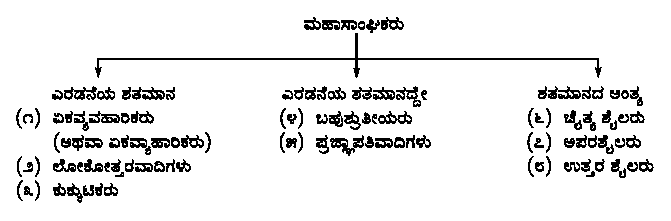
\includegraphics[scale=.95]{figures/fig1.eps}
\end{figure}
\begin{figure}[h]
\centering
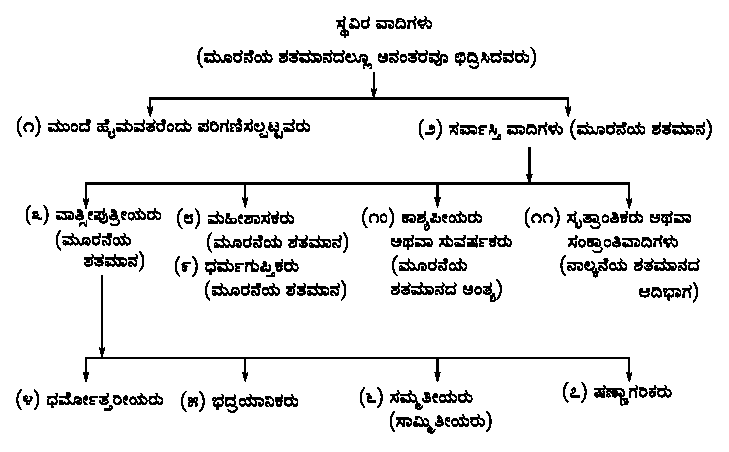
\includegraphics[scale=.87]{figures/fig2.eps}
\end{figure}

duradaqSaTxvashAtf vasumitarxna kaqti, inenxraDu ciVniV BASAMtaragaLalUlx matutx Bavayx\endnote{nAgAjuRnananunx kurita oMdu vAyxKAyxnada kataqR; `takaRjAvxlA'da kataqR kUDa.} viniVtadeVva shAkayxparxBA matutx padAmxkaraGoVSa\endnote{noVDi: obarf milalxrf, pUvoVRkatx, {\rm II pp. 4, 96-101}.} eMbavara kaqtigaLa TibeVTanf BASAMtaragaLalUlx saha aneVka vivaragaLalilx Eka matavilalx; matutx yAva paMthadiMda yAva paMtha huTiTxkoMDitu eMba viSayadalilx idamitathxM eMdu niNaRya heVLuvudu kaSaTx. pUvaRda `diVpavaMsha'da AdhArada meVle `kathAvatuthx'vina vAyxKAyxnada parxkAra mUlasaMGadiMda bwdadhx paMthagaLa utapxtitxyanunx I keLage vaNiRside:

\begin{figure}[h]
\centering
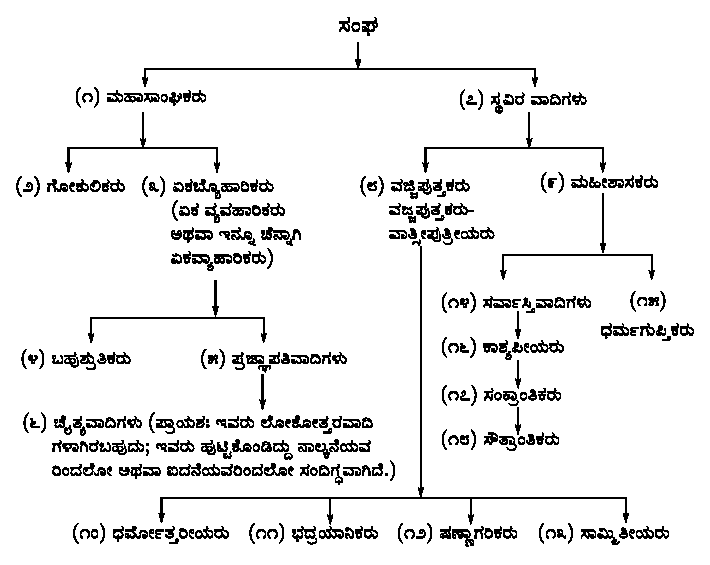
\includegraphics[scale=.87]{figures/fig3.eps}
\end{figure}
pAliVmUligaLu matAtxru paMthagaLanunx hesarisutatxve -- heYmavatiRkaru, rAjagirikaru, sidAdhxrithxkaru, pubabxseliVyaru, aparaseliVyaru, vAjiriyaru.

I vividha paMthagaLalilx, kAlakarxmeVNa kelavu pArxmuKayxkekx baMdavalalxde bahumaMdi anuyAyigaLanUnx tamageV vishiSaTxvAda sAhitayxvanUnx hoMdidadxvu. mahAsAMGika\-rige tamamxdeV Ada vinaya itutx; jatege, muMde mahAyAnigaLenisikoMDavarige ivare\break mUla. I mahAyAnigaLalilx  mAdhayxmika matutx yoVgAcAragaLeMba eraDu paMgaDa\-gaLidadxvu. ivaru tamamxdeV Ada visAtxravAda sAhitayxgaLanUnx  hoMdidadxru. sathxvira\-vAdigaLiMdalU savARsitxvAdigaLiMdalU anaMtara mUla savARsitxvAdigaLu, heYma\-vataru, mahiVshAsakaru, dhamaRgupitxkaru, matutx kAshayxpiVyaru eMba pAMthikaru huTiTx\break\-koMDaru; ivarigU saha bahuvisAtxravAda vinayx, sUtarx matutx aBidamamxgaLige\break saMbaMdhapaTaTx sAhitayxgaLidadxvu. Icina bArxhamxNasAhitayxdalilx veYBASikara mAtu barutatxde; ivaru hiMdina savARsitxvAdigaLa paMthavanunx muMduvarisikoMDu\endnote{cerfbATfsikx {\rm (Stcherbatsky). \textit{conception of Nirvana}, (Leningrad, 1927) pp. 22-23}.} baMdavareMdu BAvisalAgide. ivaru, tamamx sapxdhiRgaLAda swtArxMtikaraMtalalxde, aBidhamaR sAhitayx\-vanunx hecAcxgi avalaMbisidadxru, Adare swtArxMtikaroV aBidhamaRvu mahAguruvina mAtalalxveMdu parigaNisi keVvala sUtarxgaLanenxV avalaMbisidadxru.\endnote{veY. soVgenf {\rm (sogen)} pUvoVRkatx. pu. {\rm 101}.} samamxtiVyaru, athavA `aBidhamaRkoVshaBASayx'da saMsakxqqta pATha ulelxVKisiruvaMte `sAmimxtiVyaru', tamamxdeV Ada sAhitayxvanunx hoMdidadxMte toVrutatxde; Adare duradaqSaTxvashAtf adara bahusavxlapx BAga mAtarx `sAmimxtiVya nikAyashAsatxrX' eMba dAshaRnika garxMthada ciVNiVpAThada rUpadalilx uLidukoMDide. (nAnfjiyoV, 1272).

meVle heVLida paMgaDagaLa jatege kathAvatuthx vAyxKAyxnavu AMdarxkaroMdige (pAli -- aMdaka) pUvaRsheYlikaru matutx aparasheYlikara jatege, rAjagirikaranUnx, sidAdhxthiRkaranUnx joVDisi namUdisutatxde. adaralilx utatxra pAThakara matutx veVtulayxkara aBipArxyagaLanunx kurita mAtugaLive (ivaranunx veYpulikareMdu gurutisabahudu -- mahAyAnada oMdu viBAga `veYpulayx'); ivaranunx mahAshUnayxtAvAdigaLeMdU matutx heVtuvAdigaLeMdU kareyalAgide.

oMdeV saMGada obabx athavA aneVkara Binanx Binanx aBipArxyagaLanunx kathAtuthx namUdisutatxde matutx kathAvatuthx BASayxvu ivanunx tAnu racitavAda kAladalilx AgaleV rUpugoMDidadx paMthagaLa aBipArxyagaLeMdu heVLutatxde. bwdadhxsaMGada oDakugaLa viSayavAgi, ashoVkana satxMBashAsanagaLa pAThagaLa AdhArada meVle DA| Di.Arf. BaMDArfkarf\endnote{`ashoVka' (pariSakxqqta mudarxNa, kalakxtatx, {\rm 1932}). pu. {\rm 100}.} avarU, matutx DA| bi.eM. barua avarU\endnote{{\rm{\textit{Asoka and Hits Inscriptions} (New Age Publishers, 1955), I.} pu. {\rm 333}riMda muMdakekx.}} saha I paMthagaLu ashoVkAnaMtarada avadhiyalilx huTiTxkoMDaveMdu aBipArxyapaDutAtxre.

\begin{center}
{\textbf{\Large upadeVsha mAdhayxmagaLu}}
\end{center}

kAlakarxmeVNa I paMthagaLu tamamx upadeVshakekx yAva mAdhayxmavanunx avalaMbisi\-davu eMba viSayadalilx `vaSARgarxpaqcaCx'da kataqR padAmxkara GoVSanu bahumuKayx\-vAda saMgatiyoMdanunx namage tiLisikoDutAtxne.\endnote{noVDi: obarf milalxrf, pUvoVRkatx, pu. 99-100.} udAharaNegAgi, budadhxnu tananx anu\-yAyigaLige tamamxdeV Ada BASeyalilx upadeVshagaLanunx heVLalu anumati koTaTx\break\-neMbudu namamx tiLuvaLike baMdide.\endnote{vinayapiTaka. {\rm II. 139}.} hiVge budadhxna upadeVsha yAva yAva parxdeVsha\-gaLalilx haraDitoV AyA parxdeVshagaLa janara anukUlakekx takakxMte AyA eDegaLalilx upa\-yoVgisutitxdadx BASegaLU beVre beVreyavAgidudxvu. savARsitxvAdigaLU matutx avara\break kelavu upapaMgaDagaLU saMsakxqqtavanenxV tamamx BASege AyudxkoMDaru; EkeMdare,\break iMDiyada vAyuvayx parxdeVshagaLalilxna janaru saMsakxqqta BASeyanunx balalxvarAgidadxru.\break saMGadalilx bahusaMKAyxtarAgidadx mahAsAMGikaru pArxkaqtavanunx avalaMbisidaru.\break pArxyashaH EkeMdare tAvu parxbalarAgidadx pUvaR parxdeVshagaLalilx (magadha matutx aMga) A BASe hecACxgi baLakeyalilxtutx. vAtisxVputirxVyarAreMdare ivareV eMdu aneVka veVLe\break heVLalAda sAmimxtiVyaru vatasxdeVshadalilx parxcalitavAgidadx apaBarxMshavanunx avalaMbi\-si\-daru. sathxviravAdigaLu oMdu tarada `AMtarika' upaBASeyanunx ADutitxdadxru. mahA\-sAMGikaru ADutitxdadx BASe saha oMdu `AMtarika' upa BASeyeMdU, sAmimxtiVyara\break BASe pArxkaqtaveMdU sathxviraBASe apaBarxMshaveMdU kelavaru aBipArxyapaDutAtxre\break eMbudU saha ukatxvAgide. Adare parasapxra virudadhxvAda iveraDU mUlagaLU savARsitxvAdigaLu avalaMbisida BASe saMsakxqqtaveMbudanunx opupxtatxve. I paMthavu saMsakxqqta\-vanunx upayoVgisikoMDadadxriMda kAlakarxmeVNa mahAsAMGikara itara paMgaDagaLU idara parxBAvakekx oLagAduvenanxbeVku; tatapxriNAmavAgi Iga mahAyAnigaLa kaqtigaLe\-lalxvU saMsakxqqtadalelxV ive.

\begin{center}
{\textbf{\Large 1. sathxviravAdigaLu}}
\end{center}

budadhxna vayxkitxtavx matutx Atana upadeVshagaLa AdayxvU vishadavU saraLavU Ada citarx teVravAdi athavA sathxviravAdigaLa pAli sAhitayxdalilx kaMDubarutatxde. I sAhitayxdalilx budadhxnanunx `deVvAtideVva' athavA `sababxdeVva manusAsxnaM budodhxV BagavA' eMbu\-dAgiyU, AshacxyaRkaravAda shakitxgaLanunx hoMdu avanunx parxkaTisalu samathaRnAgi loVkaguruvAgabalalx atimAnuSaniVtaneMdU loVkoVtatxravAgi vaNiRsuva mAtu\-gaLU idaralilxve; Adare idaralilx sAdhAraNavAgi kaMDubaruva vaNaRne yAvudeMdare: budadhxnobabx mAnava, Atanige mAnavasahajavAda doVSa dwbaRlayxgaLuMTu eMbudu. Ata tananx shiSayxnobabxnige `nananx benunx noVyutitxde'\endnote{`pithithx meV AgilAyati', majijxmanikAya, seKasutatx.} eMdu heVLidAga mAnava dwbaRlayxkekx oLagAgidAdxne. matotxMdukaDeyalilx\endnote{majijxmanikAya, cAtumA-sutatx.} Ata tananx shiSayxru miVnusaMteya miVMguligaLa hAge gadadxla mADutitxdudxdanunx kaMDAga avara meVle koVpisikoMDudu namage goVcarisutatxde. Atanobabx sAmaMta rAjana maganeMdU avaru Itananunx sakaleYshacxyaR saMpatitxnoDane bahaLa mudidxniMda beLasidareMdU vaNiRsalAgide.

Ita modala bArige tananx ipapxtotxMbatatxneya vayasisxnalilx obabx muduka, obabx roVgi, oMdu heNa, matutx obabx sanAyxsi ivaranunx kaMDu I parxpaMcakekx heVsi parivArxjakatanavanunx keYkoMDaneMba asahajaveMdeV toVruva vaNaRneya saMgaDaveV I saMsAravanunx tayxjisalu Atananunx perxVrisida sahajavU neYjavU Ada matotxMdu vivaraNeyU alilxde\endnote{sutatxnipAta, padayx {\rm 936}; ``acncnxmacneUVhi vAyxrudedhxVdisAvx mAM BayaM Avisi'' (hoVrATadalilx toDagidadx janaranunx kaMDu nananxnunx Baya kaviyitu). hoVlisi: majijxmanikAyada ariya-pariyesana-sutatx.} Atanige jAcnxnoVdayavAda meVle mahA upadeVshaka matAcAyaRnAgi Ata nalavatetxYdu vaSaRgaLa kAla badukidanu. I kAladalilx Ata tananx anuyAyigaLa naDavaLikeyanunx tAnu kaMDa vivayxjAcnxnada beLakinalilx tidadxlu yatinxsidanu. baLika bahusAmAnayxvAgi elalxrigU baruva oMdu jADayxdiMda sAdhAraNa riVtiyalelxV, idara vaNaRneyalilx atimAnuSAMshagaLige EnU kaDameyilalxdidadxrU saha, maqtihoMdidanu.

budadhxna upadeVsha(dhamamx)vU kUDa, `pApadiMda dUra sari, puNayxvanunx saMpAdisu, matutx manasasxnunx shudadhxvAgirisiko\endnote{dhamamxpada, {\rm 183}.}, bahaLa saraLavU niVtiyukatxvU Agide. shiVla, eMdare oLeLx naDavaLike; samAdhi, eMdare samatoVlanavAgiruvaMte sitxmitagoLisalu aBAyxsa mADuvudu; parxjAcnx -- eMdare, nAlukx udAtatx tatatxvXgaLa (duHKa, duHKamUla, duHKoVpashama, duHKoVpashamanamAgaR) tiLivaLikeyiMda aMtarfdaqSiTxyanunx paDeyuvike; matutx udAtatxvAda aSaTxvidha sanAmxgaRvanunx aBAyxsa mADuvudu ivugaLanunx Ata otitx otitx heVLutitxdadxnu. I mAgaRvanunx Ata sadA madhayxmamAgaRveMdu kareyutitxdadxnu. EkeMdare, idu atiBoVgajiVvana matutx ati tapashiyxVlate iveraDariMDalU atatx sariditutx. Atanige kamaR matutx punajaRnamxgaLalilx naMbikeyitutx.\endnote{idanunx je.ji.jeninxMgfsx {\rm (J. G. Jennings)} tamamx {\rm \textit{Vedantic Buddbism of tbe Buddba} (Oxford University Press, 1947, Introduction, pp. xxiv xxxvi-liv)}dalilx nirAkarisutAtxre. avugaLanunx avaru bwdadhxdhamaRkekx anaMtara seVrisalapxTaTx hiMdUkAraka aMshagaLeMdu vivarisutAtxre.} Adare bariya tatatxvXjijAcnxse. udAharaNege, I vishavxda udaya matutx parxLaya iMtha viSayagaLanunx kurita caceR, Atanige seVrutitxralilalx. Ata vivarisadidadx athavA atatxkaDegiTaTx hatutx parxshenxgaLuMTu (thapeVtababx): vishavx 
\begin{enumerate}
\renewcommand{\theenumi}{\arabic{enumi}}
\renewcommand{\labelenumi}{\rm(\theenumi)}
\item anaMtakAlaviratakakxdUdxV athavA
\item idakekx aMtayxvuMTeV;
\item anaMtaveV, athavA
\item sAMtaveV; deVhavU jiVvavU
\item oMdeyeV athavA 
\item beVre beVreyeV; tathAgatanu
\item idAdxneyeV athavA
\item satatxmeVle iruvudilalxveV, athavA 
\item satatxmeVlU idUdx irutAtxneyeV; athavA 
\item Ata iruvudu eMbudu ilalxveV athavA maraNAnaMtara iruvudilalx eMbudu ilalxveV
\end{enumerate}
eMbiV parxshenxgaLu utatxravilalxde hAgeyeV uLidive. EkeMdare, oMdu pavitarx jiVvanavanunx naDesalu ivugaLiMda yAva parxyoVjanavU ilalx; anAsakitx, virakitx matutx nivARNagaLanunx paDeyalu ivu dAri toVravu. oMdu viSada aMbu obabxnanunx nATidAga Ata tananx hatitxra niMtiruva shasatxrXcikitasxkanige A BANa hoDedavana etatxraveSuTx, baNaNxveVnu. Ata yAva jAtiyavanu muMtAda viSayagaLanunx nishicxtavAgi tiLisada horatu tanage cikitesx mADabAradeMdu vidhisidare, Ata sAyuvudu KaMDita.\endnote{majijxmanikAya, cUla-mAluMkayx-sutatx.} shiVla, samAdhi, parxjAcnx ivugaLa aBAyxsadiMda obabx manuSayx tanenxlalx mAlinayxgaLanunx nAshagoLisuvudu sAdhayxvAgi ahaRta padavi hoMdalu shakayxvAgutatxde. I teradalilx Ata nivARNada parama carama sithxtiyanunx hoMdu punajaRnamxrahitanAgutAtxne.

budadhxna dashaRnavU saha tuMba saraLavAgitutx. adanunx mUru mAtugaLalilx heVLibiDabahudu: anAtamxnf, anitayx matutx duHKa nitAyxtamxveMdu heVLabahudAda yAva puruSa, athavA jiVva, jiVvAtamx athavA satatxvXvAgali ilalx Atamx eMba BAvane bariya oMdu kalapxne athavA rUDhi, asaMsakxqqta, eMdare, yAvudara berakeyU ilalxda nivARNavoMdara horatu mikekxlalx anitayx, duHKa, nitayxsatatxvXrahita, puruSaneMdU vayxkitxyeMdU nAvu sAdhAraNavAgi yAvananunx kareyutetxVvoV avanalilx parxti kaSxNavU badalAyisutitxruva nAmarUpagaLalalxde beVre matetxVnU ilalx I nAmarUpa matutx paMcasakxMdagaLu, eMdare, rUpa, shabadx, gaMdha, rasa, sapxshaR matutx bwdadhx pariBASeyalilx `dhamARyatana'veMdu kareyalAda ceVtasika viSayagaLanUnx nAvaritukoLaLxbeVku. jatege, hadineMTu dhAtugaLa tiLivaLikeyU beVku. I dhAtugaLalilx meVle heVLida hanenxraDu aMshagaLU matutx aMtariMdirxyagaLige saMbaMdhapaTaTx Aru vijAcnxnagaLu, eMdare neVtarxvijAcnxna, shorxVtarxvijAcnxna, nAsikavijAcnxna, rasanAvijAcnxna, deVhavijAcnxna matutx manoVvijAcnxna seVride.

I riVtiyAgi I vishavxda vishelxVSaNeyiMda laBisida eraDu matutx aidu mUla viBajanegaLu hanenxraDu matutx hadineMTu aMshagaLigeVrive. sathxviravAdigaLiMda kalipxtavAda vishavxda I bahuLateyanunx ivara mitarxrAda savARsitxvAda paMtha inUnx visatxriside.

aBidhamamxtathx saMgarxhada parxkAra dheVravAdada manashAyxsitxrXVya matutx neYtikadashaRnada bwdadhx keYpiDiyoMdu (idanunx eMTu hAgU hanenxraDaneya shatamAnagaLa naDuve jiVvisidadx siMhaLada sharxmeNa anurudAdhxcAyaRneMbAtanu racisidaneMdu heVLalAgide) tathate tananx paramAthaRdalilx eMdare mUlasavxrUpadalilx nAlukx, parxkAravAgide -- eMdare, citatx, ceVtasika, rUpa, nivARNa, eMdu nirUpisutatxde.\endnote{Akaqtiyalilx vaMdanA`gAtha'gaLAda meVle baruva AraMBada padayxvanunx noVDi: ``tatathxvutAtx`BidhamamxtAthx catudhA paramatathxto, citatxM cetasikaM rUpaM nibAbxNaM iti sababxthA''.} bwdadhxriMda hiVge viBajitavAda vishavxda catuviRdha viBAgagaLalilx\endnote{Aseya, rUpada, arUpada matutx atiVtada valayagaLu.} citatx 89 bageyAgide; manoVguNagaLu, eMdare ceVtasikagaLu 52 bage; BwtaguNagaLu eMdare rUpa 58 bageyAgide; rAgavimukatxvU sakala doVSarahitavU Ada nivARNa vaNaRnAtiVtavAgide.

paticaCxsamupApxda (parxtiVtayx samutApxda)veMba tatatxvXda parxkAravAgi saMsAracakarxvanunx nirUpisalAgide. udAharaNege, idu vayxkitxya oMdara meVloMdu baruva mUru (BUta-vataRmAna-BaviSayx) janamxgaLu heVge parasapxra badadhxvAgive eMbudanunx toVrikoDutatxde. bwdadhxru, cAvARkara horatu mikekxlalx BAratiVya sidAdhxMtagaLaMte kamaRvanunx naMbutAtxre matutx I kamaRveV obabx vayxkitxya baduku athavA adara muMduvarike ivakekx kAraNavAgide. kamaR mUru bage: kAyaka, vAcaka, mAnasika. koneyadanunx bwdadhxru mikekxraDakikxMtalU parxdhAnavAgi BAvisutAtxre.

kaLeda janamxdalilxna avideyx -- nAlukx AyaRsatayxgaLalilx idoMdu -- A janamxdalilx kelavu saMsAkxragaLanunx tarutatxde. hiVge gata janamxkekx saMbaMdhapaTaTx iveraDU vayxkitxyobabxnanunx vataRmAna janamxda vijAcnxnakekx oyuyxtatxve; idariMda nAma-rUpa, deVha matutx citotxVpakaraNa udaBxvisutatxve; idu muMde Aru AyatanagaLige, eMdare paMceVMdirxyagaLu matutx manasusxgaLige dArimADi koDutatxde. I Aru AyatanagaLu huTuTxkoMDa baLika avu viSaya sapxshaRkekx baLidoVrutatxve. sapxshaRdiMda hita athavA ahita, athavA hitavU alalx ahitavU alalx eMba bageya veVdane udaBxvisutatxde. vijAcnxnadiMda veVdaneyavaregina I aidu parigaLU I janamxkekx oTiTxkoMDiruvaMthavu; hiMdina janamxda avidAyx matutx saMsAkxragaLu I janamxkekx namamxnonxyuyxvaMtAdare nAvu ivugaLiMga tapipxsikoLuLxvudu asAdhayx.

veVdaneya anaMtara muMdina GaTaTx bahumuKayxvAdadudx, EkeMdare, obabx vayxkitxya BaviSayx, eMdare, Itanige punajaRnamx uMTeV ilalxveV eMbudu, I GaTaTxdalelxV nidhARravAgabeVkAdare, Ata tananx citatxda meVle hiDitavaninxTuTxkoLaLxdeV hoVgi hiDitadalilxTuTxkoMDu yAva taqSeNxyU tananxlilx udisadaMte noVDikoMDadedxV Adare, Ata mukatxnAgalu avakAshavuMTu. AdudariMda I janamxdalilx obabxna muMdina AguhoVgugaLanunx I GaTaTx niNaRyisibiDutatxde; aSuTx parxdhAnavAda GaTaTx idu. taqSeNx tananx mAgaRvanunx hiDidu eMdinaMte taledoVruvudanunx tapipxsalu Iga parxtiyobabxnU tananx ecacxrikeyalilxrabeVku. taqSeThxyiMda upAdAna eMdare hiDidukoLuLxvudu. beVku beVku eMdu keY cAcuvudu, udisutatxde; upAdAnadiMda BAva -- idanunx kamaRBAva eMdare kirxyAshiVlate, eMdu vivarisalAgide -- huTiTxkoLuLxtatxde. ivu mUrU vataRmAna janamxda kirxyAshiVla athavA saceVtanAMshagaLu (ivu hiMdina janamxda avideyx matutx saMsAkxragaLeMbaveraDakekx saMvAdigaLAgive); iveV muMdina janamxvanunx taruvaMthavu. AdudariMda BAva eMbudu `jAti'ya eMdare, muMdina janamxda mAgaRdashaRka. janamx saMbavisida meVle adu muMdina bALuveyalilx jaregU, maqtuyxvigU, goVLigU, aLivigU, duHKakUkx, viSAdakUkx, saMkaTagaLigU dArimADikoDutatxde. idanenxV saMsAracakarxveMdu vaNiRsalAgide.

I bALuve asitxtavxda mUru keSxVtarxgaLalilx vAyxpisideyeMdu bwdadhxru BAvisutAtxre: avu yAvuveMdare, 
\begin{enumerate}
\renewcommand{\theenumi}{\arabic{enumi}}
\renewcommand{\labelenumi}{(\theenumi)}
\item kAma BAvakeSxVtarx -- idaralilx keLa pArxNigaLu, BUtagaLu, nArakigaLu, rAkaSxsaru, manuSayxru, keLavagaRda kelavu nAkigaru eMdare deVvategaLu, seVrisutAtxre;
\item rUpa BAvakeSxVtarx -- idaralilx hiMdinadakikxMta meVlumaTaTxda hadinAru bageya deVvategaLidAdxre ivara madhayxdalilx janamxtALalu kelavu sAdhanegaLiMda sAdhayx: matutx 
\item arUpaBAvakeSxVtarx -- idaralilx adaqshayxrUpada deVvategaLidAdxre.
\end{enumerate}
I jiVvacakarxdalilx calisutitxruva vayxkitx I mUru keSxVtarxgaLalilx yAvudaralAlxdarU pariBarxmisutitxrabahudu.

anaMtara, muMde ELuva parxshenx EneMdare: oMdu janamxdiMda matotxMdu janamxkekx sAgutitxruva AtamxvoMdilalxdidadxre, obabxne vayxkitx hiVge eDebiDade sAgutitxdAdxne eMbudanunx daqDhapaDisuvudu heVge? oMdu janamxdiMda matotxMdu janamxkekx saMkarxmisuva yAvudAdaroMdu uMToV?

kamaRveMbudu oMdu mahAshakitx; A shakitx kuMdihoVgade iruvavaregU adu pariNAmakAriyAgiyeV irutatxde. obabx manuSayx oMdu kelasavanunx naDasabeVkeMdu Ajecnx mADidedxV Adare, Ata sAyutitxdadxrU Atana apapxNe jarugi A kelasa naDeyutatxde. hiVge, obabx vayxkitxge avasAnakAla saninxhitavAgi Atana deVha I janamxdalilx kusidu biVLutitxruvudanunx nAvu kANutitxdadxrU I janamxdalilx maqtavAgutitxruva citatx kamaRda baladiMda maruhuTiTxnalilx tananx patirUpavAgiruva matotxMdu hosa citatxvanunx hosadoMdu shariVradalilx paDedukoLuLxtatxde; idariMda kAlakarxmadalilx kamaRbalake tAnu pUNaRvAgi pariNAmakAriyAgalu anuvu doreyutatxde. kamaRbala oMdeV samavAgiruvudariMda eraDu janamxgaLU oMdaraveV eMbudu A kamaRbalada shariVra matutx citatxda upakaraNadiMda sAthxpitavAgutatxde. hiMdina janamxdalilx naMdihoVda citatxdiMda pArxpatxvAda I hosa citatxvanunx naMdihoVgutitxruva oMdu haNateyiMda matotxMda haNateyanunx hacucxva vidhAnakekx hoVlisalAgide. diVpada shiKe oMdu haNateyiMda matotxMdakekx parikarxmisalilalx, AdarU haLeya haNate neravige bArade idadx pakaSxdalilx hosa haNateya diVpada kuDi asitxtavxkekx barutitxralilalx.\endnote{noVDi: visudidhx-magagx, {\rm xvii, 163}.}

obabx manuSayxnu tananxlilx taqSeNxyudisalu avakAsha koDadidadxre, Ata bwdadhx dheyxVya\-vAda ahaRta padaviya mAgaRdalilx sAgutitxruvavanige niyatavAda shikaSxNaparxkirxyeya deseyiMda tananx jiVvitadalilx eMtha badalAvaNeyanunx taMdukoLaLxbalalxneMdare tanenxlalx sAdhAraNa kAyaRgaLU taqSaNxrahitavAgiruvaMte mADikoLaLxlu Ata samathaRnAgutAtxne. eMdare, avu `kirxyA mAtarx'vagirutatxveyeV horatu Pala koDalu avakekx avakAshaveV doreyuvudilalx. muMdina janamxgaLalilx tananx bALuveyanunx muMduvarisuva hosa kamaRgaLU udaBxvisuvudilalx. Atana pArxciVna kamaR baridAdAga Atana vataRmAna janamx tiVrihoVgutatxde Aga Atana asitxtavxvU tiVrihoVgutatxde. iMdhana mugida meVle beMkiyU ArihoVguvaMte satatxmeVle Ata elilxge hoVgutAtxno EnAgutAtxnoV namage tiLiyadu. oMdu pArxciVna garxMtha heVLutatxde: oMdu gALi birusAgi biVsidare uriyoMdu heVge naMdihoVgutatxdeyoV, yAva lekakxkUkx baruvudilalxvoV hAgeyeV muniyU saha tananx Bwtika matutx mAnasika eMdare nAmarUpagaLiMda mukatxnAgi naMdihoVgutAtxne matutx Ata yAva vaNaRnegU sikukxvudilalx.\endnote{``acicxV yathA vAta veVgeVna KitotxV atathxM paleVti na upeVti saMKaM, EvaM EvaM muniV nAmakAyA atathxM paleVti na upeVti saMKaM--sutatxnipAta {\rm (S. B. E. I88I)} padayx {\rm 1074}.}

ideV Atana `nivARNa', athavA `parinivARNa', yAva Bwtika deVhavU ilalxda nisheyxVSa nivARNa, eMdare `anupAdhisheVSa nivARNa'. obabx ahaRtanu rAga-devxVSa-moVhAdi sakala duritagaLanUnx dhavxMsamADi jiVvaMtanAgiruvAgaleV yAva `nivARNa'vanunx paDeyutAtxnoV adu `sa-upAdhisheVSa-nivARNa' mAtarx, EkeMdare Atanige inUnx BwtikashariVra uLidide.

\newpage

\begin{center}
{\textbf{\Large 2. mahiVshAsakaru}}
\end{center}

beVre beVre kAlagaLalilx adeV hesariniMda kareyalapxDuva mahiVshAsakara eraDu\break paMgaDa\-gaLive; AdudariMda I paMthakUkx savARsitxvAda paMthakUkx iruva kAlika\break saMbaMdhada viSayadalilx pAliV mUlagaLa aBipArxyakUkx vasumitarxnadakUkx vayxtAyxsa\-vide sathxviravAdigaLiMda mahiVshAsakarU vajijxputatxkarU shAKegaLAgi oDedukoMDa\break\-reMdU, mahiVshAsakariMda savARsitxvAdigaLU jatege dhamaRgupitxkarU oDamUDi\break\-koMDareMdU pAliVmUlagaLu heVLutatxve. Adare vasumitarxnu sathxviravAdigaLiMda\break huTiTxkoMDa savARsitxvAdigaLiMda mahiVshAsakaru oDamUDidareMdu nirUpisutAtxne. pArxyashaH vasumitarxnu hiMdina matutx anaMtarada mahiVshAsakaranunx berasikoMDadadx\-riMda I saMdigadhxkekx oLagAgidAdxneMdu toVrutatxde.

hiMdina mahiVshAsakaru rAjagaqhadalilx modalaneya saMGavu EpaRTaTx kAlakekx seVridavareMdu heVLabahudu. purANaneMba hiriya sharxmaNanu dakiSxNAgiriyalelxV niMtubiTaTxneMdU mahAkAshayxpanu karedidadx pariSatitxge Ata baralilalxveMdU nAvu I hiMdeyeV heVLidedxVve Atana anuyAyigaLu mahiVshAsakareMba oMdu paMgaDavanunx kaTiTxkoMDareMdu kANutatxde. avaru tamamxdeV Ada vinayxgarxMthavanunx hoMdidadxru: adaralilx vivAdAsapxdavAgidadx ELu niyamagaLanunx seVrisalAgididxtu. mahiVshAsaka vinayavu purANanige eraDaneya sAthxnavanunx koTuTx kwMDinayxnige modalaneya sAthxnavanunx koDutatxde. I paMthavU saha sathxviravAdigaLa saMcAramAgaRvanenxV hiDidu, eMdare kwshAMbi, avaMtigaLa mUlaka utatxra kananxDada banavAsiya dAriyanunx hiDidu siMhaLavanunx seVritu. banavAsiya rANiyobabxLu mahiVshAsakarige oMdu satxMBa matutx oMdu vihAravanunx dAnavAgi koTaTxLeMdu nAgAjuRnakoMDada shAsanavoMdu tiLisikoDutatxde. siMhaLadalilx I paMthavitetxMdu PAhiyAnf heVLutAtxne. jAtaka `AThamxkathA' eMbudaralilx I pArxsAtxvika sholxVka goVcarisutatxde:

\begin{center}
mahiVshAsaka vaMshaMhi saMBUteVna nayaNuNxnA\\
budadhxdeveVna ca tathA BikukxnA sudadhxbudidhxnA
\end{center}
(mahiVshAsana vaMshadavanU shudadhxbudidhxyU nayakoVvidanU Ada budadhxdeVvaneMBa sharxmaNa nananxnunx I garxMtha racanege koVridAdxne.)

pArxciVna mahiVshAsakara sidAdhxMtagaLu sathxviravAdigaLavugaLoDane sahajavAgiyeV oDaMbaTiTxve; utatxra mahiVshAsakaravoV hecAcxgi savARsitxvAdigaLavaMteyeV ive. sathxviravAdigaLaMteyeV pUvaRda mahiVshAsakaru EtatfkaSxNadalilx paramasatayxvanunx sAkASxtakxrisikoLaLxbahudenunxtAtxre. avara aBipArxyadalilx BUtaBaviSayxgaLilalxveV ilalx; Adare vataRmAnavU adaroMdige asaMsakxqqtarU idedxV irutAtxre; saMsakxqqtaru layahoMdutAtxre. asaMsakxqqta dhamaRgaLU oMBatutx

\begin{enumerate}
\renewcommand{\theenumi}{\arabic{enumi}}
\renewcommand{\labelenumi}{(\theenumi)}
\item parxtisaMKAyxniroVdha, eMdare, jAcnxnadoMdige tiVruvike;
\item a-parxtisaMKAyxniroVdha, eMdare jAcnxnarahitavAgiyeV, eMdare sahajavAgi kAraNagaLu tiVrikoLuLxvudariMda tiVrikoLuLxvudu;
\item AkAsha;
\item  aneVknagxtA eMdare avicAlayxte;
\item[(5-7)] kushaladhamaR tathAtA, akushaladhamaR tathatA, matutx avAyxkaqtadhamaR tathatA, eMdare, puNayxkaravAda dhamaRgaLa tathate, apuNayxkaravAda dhamaRgaLa tathate, matutx puNayxvU apuNayxvU alalxda dhamaRgaLa tathate; 
\item [(8-9)] mAgARMga tathatA matutx parxtiVtayx samutAbxda tathatA, eMdare mAgaRda oMdu lakaSxNavAda thathate matutx avalaMBanadiMda huTiTxkoLuLxva dhamaRda tathate, I oMBatatxra paTiTx mahAsAMGikara paTiTxyoMdige aMshataH sarihoVlutatxde.
\end{enumerate}

I paMthada muKayx sidAdhxMtagaLAvaveMdare: sorxVtApananxrige niVcagatiyuMTu, Adare puNAyxpuNayxkamaRgaLigoLagAgada ahaRtaru adakekx oLagAguvudilalx; yAva deVvategAdarU saha pavitarx jiVvanavanunx naDesalu asAdhayx; I bwdadhxdhamaRvanonxlalxda pASaMDige apArxkaqtashakitxgaLu odagavu; I janamxkUkx muMdina janamxkUkx naDuve matAtxva aMtara asitxtavxvU iruvudilalx; saMGadalilx budadhxnU seVridAdxne, AdudariMda saMGakekx koDuva dAna mahAsherxVyasakxraveV horatu budadhxnige koTaTxdudx sherxVyasakxravenisadu; oMdu loVkadiMda matotxMdu loVkakekx hoVguva yAvudoMdu ilalx eMbu\-daMtU nishacxya.

`kathAvatuthx'vu beVreyavoMdige I paMthada aBipArxyagaLanUnx namUdisutatxde; adara parxkAra ivaru BAvisidudxdeVneMdare lwkika vicAragaLalilx obabx vayxkitxya `sharxdedhxVM\-dirxya' matutx adaraMthavu ilalx {\rm (XIX. 8)}. AyaR aSATxMgamAgaRdalilx nija\-vAgiyU aidu aMgagaLu mAtarx iveyeV horatu saMyakfvAkf, saMyakfkAyaR, saMyakf\-jiVvana ivu A-citatxvAdudariMda ivugaLige alilx jAgavilalx. {\rm (XX. 5)}

I paMthadavara aBipArxyagaLa viSayadalilx vasumitarxnigU BASayxsahitavAda `kathAvatutx'vinalilxruva nirUpaNegU hecAcxgi sAmayxviruvudu kutUhalajanakavAgide. idoMdu soVjiVga -- utatxra mahiVshAsakara matasidAdhxMtagaLu pArxciVna mahiVshAsakara aneVka sidAdhxMtagaLige virudadhxvAgive. savARsitxvAdigaLaMte ivarU saha BUta, BaviSayx matutx aMtarABAvagaLalilx vishAvxsaviDalu modaliTaTxru. sakxMdhagaLu, dhAtugaLu, matutx AyatanagaLu yAvAgalU biVjarUpadalilxrutatxveyeMdU; `vitakaR' matutx `vicAra'gaLu (parxthamAnavxya matutx AloVcane) oMdaroDanoMdu beredukoLuLxtatxveyeMdU muMtAgi avaru parxtipAdisidaru.
\begin{center}
{\textbf{\Large 3. savARsitxvAdigaLu}}
\end{center}

savARsitxvAdiV paMtha theVravAdiV paMthakekx samiVpavAgi hoMDikoMDide. ivareV mikekxlalx paMtha paMgaDagaLigiMtalU hecAcxgi theVravAdigaLige bahu hatitxravAgiruvavaru. konege, kirx.sha. mUraneya shatamAnadalilx (eMdare, ashoVkana kAladalilx jarugida mUraneya saMGakekx savxlapx muMce) savARsitxvAdigaLeMba hesaranunx paDeda I paMthada aBipArxyagaLu budadhxna kAladaSuTx hiMdakekx hoVgutatxve eMdu toVrutatxde. `sababxM atithx' (elalxvU idedxV ide) eMba BAvane `saMyukatxniNaRya' {\rm (IV-15)}\endnote{hoVlisi: majijxmanikAya, {\rm I. 3}.}dalilx goVcarisutatxde; aDuTx haLeyadu idu. I paMthavU sathxviravAdiV paMthavU asitxtavx sidAdhxMtadavu. ivarige I bahiHparxpaMcavU adara dhamaRgaLU nijavAda asitxtavxvanunx paDediruvaMthavu. AdudariMda I paMthadavaru samasatxvU hiMdeyU itutx, iMdU ide, muMdeyU aviratavAgi irutatxde eMdu naMbutATxre. I paMthadavaru parxtipAdisutitxdadx kelavu aMshagaLanunx mAtarx `kathAvatuthx' namUdisutatxde; idariMda, I paMtha rUpugoLuLxtitxruvAga sathxviravAdadiMta adu dUra saridiralilalxveMbudu goVcarisutatxde. kathAvatuthx BASayx heVLuvudeVneMdare:\endnote{noVDi: esf,jaDf.aMgf {\rm (Aung)} matutx shirxVmati rihxsf DeVviDfsx {\rm (Rhys Davids). \textit{Paints of Controversy} (P. T. S., 1915), xix: 1.2; 1.6.7; II. 9; XI.6}.} I paMthadavaru tathayxgaLa parxveVsha karxmeVNa uMTAgutatxde, sathxviravAdigaLu heVLuvaMte EkakaSxNadalilxlalx; majijxVputitxVyaru (vAtisxV putitxVyaru?), sAmimxtiVyaru, matutx ahaRtara pArxbalayxkekx edurubidadx mahAsAMGikaralilx kelavaru ivara jatege I paMthavU saha ahaRta padaviyiMda ahaRtanobabxnu keLaguruLabahudeMbudanunx parxtipADisutatxde.

vasubaMdhu eMbAtanu I paMthada atayxMta sherxVSaThx parxsAthxnakAra. `aBidhamaR'da meVlaNa jAcnxna parxsAthxnaveV modalAda ELu mUla garxMthagaLanunx avalaMbisi Ita `aBidhamaRkoVsha'veMba saMsaMGaTita garxMthavanunx racisidanu. muMdina dinagaLalilx pArxmuKayxkekx baMda veYBaSikaru, kelavara aBipArxyada parxkAra,\endnote{cerfbATfsikx, pUvoVRkatx, pu. {\rm 22-23}.} savARsitxvAda paMthavanunx muMduvarisidaru; Adare yavakAmisoVgenf\endnote{pUvoVRkatx, pu. {\rm 102,113}.\\ * anaMtara avanobabx parxmuKa yoVgAcAriyAda.} eMbAtanu idoMdu savARsitxvAdigaLa shAKeyeMdeV heVLutAtxne. vasubaMdhu obabx veYBASika; mUla aBidhamaR garxMthagaLa vAyxKAyxnavAda `viBASA' eMbudariMda `veYBASika' eMba pada huTiTxkoMDide. Itana vAyxKAyxnakAranAda yashoVmitarxnAdaroV swtArxMtikanu, eMdare, aBidhamaRvu budadhxparxBuvina mAtalalx eMdu gaNisi sUtarxgaLanunx mAtarx avalaMBisidadxvanu.

`hadineMTu paMthagaLa' cariteyanunx bareda vasumitarxnu savARsitxvAdigaLu\break hoMdidadx Binanx Binanx aBipArxyagaLadoMdu paTiTxyoMdanunx koDutAtxne. BAratada sathxviravAdigaLu savARsitxvAdigaLige karxmeVNa eDegoDutAtx hoVdaru; I savARsitx\-vAdigaLu muKayxvAgi hiMdina paMthagaLa pakaSxvanunx hiDidu, budadhxru elalx tarada atimAnuSa shakitxgaLigU AkarareMdu parxtipADisutitxdadx parxbalarAda mahAsAMGikara paMthadoDane hoVrADuvudaralilx niratarAgidadxru. AdudariMda I paMthadaveMdu vasumitarxnu namUdisuva aBipArxyagaLanunx nAvu mahAsAMGikara athavA avara samakAliVna paMthagaLa aBipArxyagaLa beLakinalilx aritukoLaLxbeVku. vasumitarxna I paTiTx kathAvatuthxvina kaladiMda eMdare, mUraneya shatamAnada madhayxBAgadiMda, Avarege I paMthadalilx uMTAda beLavaNigeyanu saha toVrisutatxde. ililx nAvu bahumuKayxvAda kelavaMshagaLanunx mAtarx koDabahudu''

I paMthada matada parxkAra, ahaRta padaviyiMda ahaRtaru cuyxtarAgabahu\break\-deMbudanunx nAvu meVle kaMDidedxVve. Adare sorxVtApananxrige eMdare, bwdadhxpaMthadalilx ahaRta padaviya parxthama GaTaTxvanunx talupidavarige, iMtha cuyxtiyilalxveMdu ivaru nirUpisuvudoMdu kwtuka. sathxviravAdigaLa hAge, Adare mahAsAMGikarige virudadhx\-vAgi, I paMthavU saha atimAnuSashakitxgaLiveyeMbudanunx opupxvudilalx, mahAsAMGi\-karu parxtipAdisuvaMte I paMthadavarU saha I dhamaRda savaRvanunx omemxgeyeV budadhxru tiLisalArareMdU, avara sUtarxgaLalilx parxtiyoMdU niduRSaTxvAgide eMdu heVLalAgadeMdU, avara parxtiyoMdu mAtU `niVtAthaR'vAdudeMdu, eMdare parama satayxvanenxV nirUpisuvaMthadeMdu heVLalu bAradeMdU heVLutAtxre. savxtaH budadhxreV kelavu sUtarxgaLu a-niVtAthaRgaLeMbudanunx opipxkoMDidAdxre. inunx muMde, mahAsAMGikara aBipArxyakekx virudadhxvAgi, ivaru samAdhisithxtiyalilxruvAga yAvobabxnU oMdu shabadxvanUnx uvAcxramADalAguvudilalx matutx A sithxtiyalilxdAdxga Ata maqtihoMduvudU ilalx, eMdu parxtipAdisidaru.

sathxviravAdigaLa hAge, ivarU saha barxhamxcayaR (eMdare pavitarx jiVvana)\break deVvategaLigU sAdhayx eMdu naMbidadxru -- mahiVshAsakarigU sAmimxtiVyarigU ida\-ralilx vishAvxsaviralilalx -- matutx satatxvX (iruvike). upAdAnada (hiDidukoLuLxvudara) muMduvarikeyeV horatu matetx beVreyalalx eMba aBipArxyavanunx hoMdidadxru. boVdhisatavxrU saha inUnx sAmAnayx manuSayxreV (paqthakf jana), EkeMdare ava\-rinUnx `saMyoVjana' (shaqMKale)gaLanunx kaLedukoMDilalx. ahaRtarigU saha tAvu kaliya\-beVkAdadudx ide, avarU tamamx pArxciVna kamaRPaladiMda mukatxrAgilalx. `saMsakxqqta dhamaR'\-venisida heVtu niyamakUkx {(\rm Law of Causation)} avaroLapaTiTxdAdxre matutx avara kelavu kAyaRgaLu puNayxkaravAgiyU irabahudu. elalx anushayagaLU (oLagaDa\-giruva duSapxrXvaqtitxgaLu) `ceYtasika'gaLeV. avu `citatxsaMparxyukatxgaLu' (citatxdoDane beredu\-koMDiruvaMthavu). taqSaNx matutx rUpaBUyiSaThxvAda loVkadalilx mAtarx `aMtarABAva' (naDuvaNa iravu) nishicxtavAgi uMTu. `anAsarxvavAda' (keLa eLatagaLilalxda) `vitakaR' (manasasxnunx oMdu viSayakekx hacucxvudu)voMduMTu -- (idanunx mahiVshAsakaru opupxvudilalx. vitakaR sAsarxvavAdudeMdeV avareNike.) bwdadhxmatavanonxlalxda pAKaMDigaLU saha aidu `Qudidhx'gaLanunx (atimAnuSashakitxgaLanunx) paDeyabahudu.

saMkarxmisuva `lwkika pudagxla'gaLuMTu. Adare idu obabxna jiVvitAvadhiya saMsAkxragaLige anavxyisutatxde. nAlukx `loVkoVtatxra dhAyxna'gaLU uMTu; nAlukx mUlaBUtavAda dhAyxnagaLige koTaTx hesaridu.

vayxkitxyobabxna `neYrAtamxyX'vanunx savARsitxvAdigaLu etitxhiDiyutAtxre; Adare padAthaRgaLa shAshavxtafAda asitxtavxvanunx avaru opupxtAtxre. sathxviravAdigaLa hAge savARsitxvAdigaLU I vishavx aneVka mUla darxvayxgaLiMda nimiRtavAgide eMba sidAdhxMtavanunx avalaMBisidAdxre. ivara parxkAra, aidu sakxMdhagaLu, hanenxraDu AyatanagaLu matutx hadineMTu dhAtugaLa jatege eraDu vagaRgaLAgiruva epapxtetxYdu dhamaRgaLu, eMdare, epapxtetxraDu saMsakxqqta (upAhita athavA joVDisiruva) dhamaRgaLu matutx mUru asaMsakxqqta (anupAhita) dhamaRgaLu -- AkAsha, parxtisaMKAyx niroVdha, matutx aparxtisaMKAyxniroVdha -- uMTu. epapxtetxraDu saMsakxqqta dhamaRgaLanunx nAlukx vagaRgaLAgi viMgaDisalAgide: rUpa (vasutx) -- avijacnxpitxrUpavU seVri hanonxMdu bage; citatx oMdu, eMdare kAyaR rUpadalilx parxkaTavAguvudakekx muMcina citatxmuderx; nalavatAtxru citatxsaMparxyukatx dhamaRgaLu; hadinAlukx citatx parxyukatx dhamaRgaLu. I vagiVRkaraNakUkx sathxviravAdigaLa vagiVRkaraNakUkx vayxtAyxsavide eMbudu gamanAhaRvAgide. hiMde heVLidaMte, sathxviravAdigaLu mUladhamaRgaLanunx nAlukx vagaRgaLAgi viBajisutAtxre. ililx hosadAgi vasutxgaLigAgali citatxkAkxgali saMbaMdhapaDada citatxviparxyukatx dhamaRveMba vagaR kANisikoLuLxtatxde. avu yAvAgalU parxkaTavAgade gUDhavAgiruva shakitxgaLeMdu yamakAmi shoVgenf\endnote{pUvoVRkatx, pu. {\rm 159}.} avaru heVLutAtxre. yAvudAdarU oMdu vasutx athavA mAnasika AdhAravanunx avalaMbisada horatu avu ceVtanagoLaLxlAravu eMbudanunx nAvu gamanisabeVku. iveraDariMdalU ivu beVreyAgiyeV ive. AdudariMda ivakekx beVroMdu upanAmadheVyaveV ide: rUpa, citatx viparxyukatx saMsAkxradhamaRgaLeMdu.

I epapxtetxraDu dhamaRgaLu oMdakokxMdu beVre beVreyAgidadxrU, hatutx heYtuka saMbaMdhagaLiMda, eMdare Aru parxdhAna heVtugaLu matutx nAlukx gwNa heVtugaLu athavA `parxtayxya'gaLiMda badadhxvAgive.

I teradalilx, sathxviravAdigaLa hAge, I paMthavU saha obabx vayxkitxyAgali vishavxvAgali meVle heVLida vagaRgaLalilx oMdaradoV matotxMdaradoV Ada dhamaRgaLiMda AgideyeV horatu matAtxvudariMdalU alalx eMdu sidAdhxMtisutatxde eMbudU, matutx ivalilx ibabxgeya racanegaLidudx vishavxdalilx rUpa(vasutx)vU vayxkitxyalilx vitatxvU parxbalataravAgive eMbudU namage tiLidubarutatxde. rUpa(vasutx)vu paqthivx, apf, teVjasf matutx vAyugaLeMba nAlukx mahABUtagaLa saMkalana. vayxkitxyU vishavxvU tamamx bahisasxvXrUpadalilx saMtatavAda badalAvaNege IDAgutAtxre, (Adare tamamx aMtaHsatAvxMshadalalxlalx); vataRmAna parisithxtiyanunx BUta nidhaRrisutatxde, bataRmAna BaviSayxda nidhARrakavAgide. I riVtiyalilx nAvu eMdeMdigU huTuTx hAkutatxleV eMdeMdU badalAvaNe hoMdutatxleV sAgutitxdedxVve. namamxlilx avikAriyU shAshavxtavU Ada AtamxvoMdanunx sAthxpisuvudu anavashayxka; EkeMdare BUtakUkx vataRmAnakUkx BaviSayxkUkx iruva aviciCxnanxvAda saMbaMdha namamx gurutanunx aLisi hAkade kApiDutatxde.\endnote{noVDi: je. takAkusu {\rm (Takakusu), \textit{The Essenitals of Buddbist Pbilosophy} (University of Hawaii, 1947), p. 72}.}

kAshimxVradalUlx gAMdhAradalUlx habibx aBivaqdidhxsida I paMthakekx kAniSakxnu poVSakanAgidadxnu. I arasana kAladalelxV oMdu bwdadhx pariSatutx  seVritutx matutx sUtarx, vinaya, matutx aBidhamaRgaLa meVle oMdoMdakUkx lakaSx sholxVkagaLu racitavAdavu. BASayxgaLu racitavAda meVle rAjanu tAmarxPalakagaLa meVle ketitxsidaneMdU avugaLanunx peTiTxgegaLalilxrisidadxneMdU heVLalAgide.\endnote{yuvAnf cAvxMgana parxmANadiMda.} sUtxpagaLa taLadalilx hugiduhoVgiruva ivu eMdAdaroMdu dina patetxyAdAvu.

I paMthakekx `heVtuvAdi'gaLeMdU hesaruMTu.

\begin{center}
{\textbf{\Large 4. heYmavata paMtha}}
\end{center}

himAlaya parxdeVshagaLa heYmavatapaMthavu sathxviravAda paMthada utatxrAdhikAri\-yeMdu vasumitarxna heVLike. Adare I paMthada sidAdhxMtagaLanunx, adaralUlx bwdadhxsaMGadalilx modalu birukanunx birisida aidu aMshagaLanunx, nAvu parishiVlisidedxV Adare vasumitarxna heVLikeyanunx parigaNisutAtxre eMbudu kutUhalajanakavAgide; pirxjilusikxyoV avareV ivaru enunxtAtxne.\endnote{noVDi: nalinAkaSxdatf, {\rm{\textit{Early Monastic Buddhism}, II, }} pu. {\rm 169-70}.} savARsitxvAdigaLa hAge I paMthavU saha boVshisatatxtXrige hecicxna pArxshasatxyXvanunx koDalilalx; avaranunx paqthakf jana (sAdhAraNa jana) eMdeV ivaru BAvisidaru; Adare, savARsitxvAdigaLaMtalalxde, vidhamiVRyarU saha atimAnuSashakitxgaLanunx paDeyabalalxreMbudanUnx athavA deVvategaLu pavitarx jiVvanavanunx (barxhamxcayaRvanunx) naDasabalalxreMbudanUnx ivaru opapxlilalx.

\begin{center}
{\textbf{\Large 5. vAtisxVputirxya paMtha}}
\end{center}

Bwdadhxra peYki vAtisxVputirxVyaru `pudagxla' eMba nitayxvasutxvoMdaralilx tamage\break naMbikeyuMTeMdu heVLutAtx tAveV oMdu parxteyxVka paMgaDavAgi niMtaru. upa\-paMthiVyarAda sAmimxtiVyareMbavarU ivarU oMdeV eMdu etitx heVLalAgide.\endnote{`vAtisxVputirxVyA Arayx-sAmimxtiyAH' -- suPxTathAR (japAni mudarxNa), pu. {\rm 699}, salugaLu {\rm 3--6}.} tananx `aBidhamamxkoVsha'da aMtayxdalilx vasubaMdhuvu vAtisxVputirxVya paMthadavara AtamxsidAdhxMtavanunx KaMDisalu oMdu adhAyxyavanenxV miVsalAgirisidAdxne. iMtha oMdu `pudagxla'vilalxde janamxdiMda janamxkekx jiVva sAguvudeV asAdhayx eMdu avara naMbike. idu sakxMdhagaLU sakxMdhagaLalalxdeyU alalx. ivara matada parxkAra kelavu saMsAkxragaLu kelavu kAla irutatxve. matetx beVreyavu parxtikaSxNadalUlx nAshahoMdutitxrutatxve. aidu AshacxyaRkaravAda shakitxgaLanunx vidhamiVRyarU saha hoMdabalalxreMbudanUnx matutx ahaRta padaviyiMda ahaRtanu cuyxtanAgabalalxneMbudanUnx savARsitxvAdigaLa hAge I paMthadavarU saha opipxkoMDidadxru.

itara upapaMthagaLu, eMdare, dhamoVRtatxriVyaru, BadarxyAnikaru matutx SaNANxgarikaru ivaralilxna parasapxra vayxtAyxsagaLu ahaRta, Atana cuyxti, Atana jAcnxna matutx saMshayagaLu ivugaLa viSayadalilxna oMdu padayxda kelavu kelavu sAlugaLanunx beVre beVreyAgi vAyxKAyxnisuvudaralilx mAtarx niMtive.

`pudagxla'da meVle I paMthadavara sharxdedhxyanunx kaMDu, ivaranunx bwdadhxreMdu parigaNisabahudeV eMba parxshenx padeV padeV ELutitxde. kelavu sUtarxgaLalilx baruva `AtAtx' athavA `AtAmx' eMbudanunx kelavaru tamamx `AtamxsidAdhxMta'vanunx nirUpisuvudakAkxgi etitxkoLuLxvaMteyeV, ivarU saha tamamx sidAdhxMtavanunx poVSisalu bwdadhxsUtarxgaLalilx halavAru eDegaLalilx kaMDubaruva `pudagxla' eMba shabadxvananxSeTxV, adara parxkaraNAthaRvanunx gamanisadeyeV, avalaMbisutAtxre. jatege `kathAvatuthx'vu, mikakxvugaLoMdige I keLagaNa `aBipArxyagaLanunx sAmimxtiVyaradeMdu nidashiRsutatxde: deVvategaLu unanxta jiVvitavanunx naDesalAraru. rUpaloVkada deVvategaLigU kaNuNx, kivi, mUgu, nAlage, shariVra, matutx citatxgaLeMba Aru iMdirxyagaLuMTu. aMtarABava matutx vijicnxpitx (parxvacanakAyaR)gaLU saha neYtikavAgi pariNAmagaLAgive. aBidhamaRda anuyAyigaLa parxthama matutx divxtiVya GaTaTxgaLa naDuve, eMdare `vitakaR' mAtarx naMdihoVgi `vicAra' inUnx uLidukoMDiruva eDeyalilx oMdu dhAyxnada GaTaTxvU uMTeMdu nAvu BAvisabeVkenunxtAtxre. mahiVshAsakaraMte, AyaR aSaTxMgika mAgaRdalilxna saMyakfvAkf, saMyakfkirxyA matutx saMyakf jiVvanaveMba mUru aMgagaLU vAsatxvasithxtigaLeMdU mAnasika sithxtigaLalalxveMdU ivarU aBipArxyapaDutAtxre.

\begin{center}
{\textbf{\Large 6. dhamaRgupitxkaru}}
\end{center}

mahiVshAsakara oMdu shAKeyAda dhamaRgupitxkaru kelavu saNaNx aMshagaLalilx mAtarx avariMda BinanxrAgidadxru. Adare, avarige avaradeV Ada sUtarx, vinayx matutx aBidhamaRsAhitayxvitutx. madhayxESAyx matutx ciVnAgaLalilx I paMtha janara pirxVtiyanunx gaLisitu matutx idara pArxtimoVkaSxvanunx ciVnAdeVshadavaru sivxVkarisidaru. budadhxnU seVrikoMDiruva pUNaR saMGakekxV dAnadhamaRgaLanunx mADabeVkeV athavA budadhxnige parxteyxVkavAgiyeV eMbaMtha kelavu saNaNx vicAragaLalilx I paMthadavarigU mahiVshAsakarigU BinAnxBipArxyavitutx. eraDaneyadu idakekx samamxta matutx sUtxpagaLige datitxgaLanunx koTaTxrU adu puNayxkAyaRveMdu idu eNisitutx. idanunx AMdharxkara ceYtayx paMthavu nirAkarisitutx. mahiVshAsakara hAge. dhamaRgupitxkapaMtha saha yAva vidhamiRgU atimAnuSa shakitxgaLu doreyaveMdU naMbitutx.

\begin{center}
{\textbf{\Large 7. kAshayxpiVyaru}}
\end{center}

sAthxvariVyareMdU, sadadhxmaRvaSaRka athavA suvaSaRkareMdU kareyalapxDutitxdadx kAshayxpiVyaru savARsitxvAdigaLu matutx dhamaRgupitxkariMda kelavu gwNa aMshagaLalilx BinAnxBipArxyavanunx hoMdidadxru matutx sathxviravAdigaLoMdige miLitarAgidadxru. AdudariMda ivarige sAthxvariVyareMdu hesarAyitu. mikekxraDu hesarugaLu TibeTiTxna mUlagaLalilx goVcarisutatxve. I paMthavU saha tanagU parxteyxVkavAgi oMdu sAhitayxvide eMdu heVLikoLuLxtatxde.

I paMthada parxkAra, Palisida pArxciVna kamaRvu uparatiyanunx hoMdide; inUnx Palakekx bArada pArxciVnavu jiVvaMtavAgiyeV muMduvariyutatxde. I BAvane savARsitxvAdigaLa neleyanunx tidudxtatxde; avaru heVLuvudeVneMdare, BUta matutx BaviSayxgaLu vataRmAnadoMdige seVrikoMDeV irutatxve eMdu.

\begin{center}
{\textbf{\Large 8. saMkArxMtivAdigaLu athavA swtArxMtikaru}}
\end{center}

saMkArxMtivAdigaLu kAshayxpiVyariMda udaBxvisidareMdU saMkArxMtivAdigaLiMda\break swtArxMtikaru huTiTxkoMDareMdU pAliV mUlagaLiMda tiLidubarutatxde; Adare vasu\-mitarxnu iveraDU oMdeV eMdu heVLutAtxne. aBidhamaRvanunx parxmANagarxMthavanAnxgi parigaNisade sUtarxgaLanunx mAtarx ivaru avalaMbisidadxriMda swtArxMtikaranunx veYBASikara edurALigaLeMdu pariBAvisalAgide. vasubaMdhuvu sAmAnayxvAgi veYBASikara kaDege olididadxrU I aBipArxyadalilx mAtarx swtArxMtikaranunx etitx hiDiyutAtxne.\endnote{enf. datf, pUvoRVkatx, {\rm II}. pu. {\rm 168}.} `daqSATxMta\break\-paMki' athavA `daqSATxMtamUlashAsatxrX'da kataqRvAda kusUralabadxnu dASATxRMtikara\break mUla guru matutx budadhxnu tiVrikoMDa nUru vaSaRgaLa naMtara bALidavanu. I paMthada eraDaneya vAyxKAyxtanAda shirxVlabadhxnoV budadhxna taruvAya nAnUru vaSaR\-gaLa meVle janamxtALidadxvanu.

yAva upadeVshadiMda I paMtha swtArxMtikaveMba hesaranunx paDeyitoV A upadeVsha yAvudeMdare; tamamx sUkaSxmXrUpadalilx sakxMdhagaLu oMdu loVkadiMda matotxMdu loVkakekx saMkArxMtisutatxve eMbudu; Adare sAmimxtiVyaru saMkArxMtisuva aMsha pudagxlaveV horatu matetxVnU alalx enunxtAtxre. nAlukx `mUlAMtika sakxMdha'gaLige matutx idakekx mUlavAda sUkaSxmXcitatxsavxrUpada `EkarasasakxMda'voMdide. ideV `EkarasasakxMdha' enanxbahudAda `paramAthaRpudagxla' eMbudeV oMdu janamxdiMda matotxMdu janamxkekx saMkArxMtavAgabalalxMthadu. I sUkaSxmXcitatx mahA sAMGikaru heVLuva deVhavanenxlalx vAyxpisikoMDiruva citatxkekx sarihoMdutatxde. yoVgAcAraru nirUpisuva AlayavijAcnxnavU idU oMdeV. AdudariMda I Ekarasa sakxMdha sidAdhxMtavanunx I paMthavu mahAsAMGikariMda parigarxhisi yoVgAcArapaMthakekx eravalAgi koTiTxtu eMdu Uhisalu sAdhayx. parxtiyobabx sAdhAraNa manuSayxnalilxyU saha tAnu budadhxnAgabalalx satatxvXvide eMdu I paMthavU saha naMbutatxde. parxtiyoMdu jiVviyalUlx saha budadhx biVjarUpadalilxdAdxne eMba mahAyAna paMthada tatatxvXkekx I sidAdhxMta munUsxcaneyaMtide enanxbahudu. iMtha daqSiTxgaLanunxLaLxdAdxgiruvudariMda, I paMthavu oMdu kaDe shArxvakAyAna athavA hiVnayAnakUkx matotxMdu kaDe mahAyAnakUkx seVtuveyAgide eMdu pariBAvisalAgide. I saMkArxMtivAdigaLige tAmarxshATiVyareMdU hesaride; pArxyashaH avaru uDutitxdadx keMpu baTeTxyiMda avarige I hesaru baMdirabahudu.\endnote{adeV, {\rm II}. pu. {\rm 49}.}
\begin{center}
{\textbf{\Large 9. satayxsididhxpaMtha}}
\end{center}

madhayxBAratadalilx jiVvisutitxdadx harivamaR eMbAtanu sAthxpisida satayxsididhx eMba matotxMdu paMthavuMTu oMdu ciVnAmUlavu (sanf-yinf)\endnote{veY. soVgenf, pUvoRVkatx, pu. {\rm 175}.} Ita niyARNada 890 vaSaRgaLAcege janamx tALidavaneMdu heVLutatxde. Ita kAshimxVrada hiVnayAni\-gaLa muKaMDanada kumAralabadhxna paTaTxshiSayx. kelavaru Itananunx bahushurxtiVyara anu\-yAyiyeMdU, matetx kelavaru Itanobabx swtArxMtika athavA dhamaRgupitxkaneMdU heVLutAtxre. mahAyAnada neravugoMDu Ita hiVnayAna sidAdhxMtakekx aMTikoMDi\-dAdxneMdu inUnx kelavaru heVLutAtxre. vasutxgaLalilx alalxdidadxrU vayxkitxyalilx Atamx eMbu\-dilalxveMdu (Atamx-neYrAtamxyXvAda) savARsitxvAdigaLu vAdisidaru. harivamaRnoV neYrAtamxyX eMbudanunx eMdare dhamaRneYrAtamxyXvanunx titxhiDidanu; idu mahAyAnada oMdu lakaSxma. loVkadalilx 84 dhamaRgaLive, Adare ivu nitayxgaLalalx. saMvaqtisatayx matutx paramAthaRsatayx eMbudAgi satayxvu eraDu bageyAgide eMba sidAdhxMtavanunx Ita boVdhisidanu; matutx Atamx sAMparxdAyikavAgi ideyeV horatu nijavAgi adu ilalxveV ilalx eMdU upadeVshisidanu. hiVnayAnigaLa `budadhxkAya' sidAdhxMtavanunx Ita sivxVkarisidanu matutx dhamaRkAyavu shiVla, samAdhi, parxjAcnx, vimukitx matutx vimukitxjAcnxnadashaRnaveMdu aidu bageyAgideyeMdu vivarisidanu. Adare budadhxnige hatutx balagaLu, nAlukx veYshAradayxgaLu, mUru bageya samxqqtuyxpasAthxnagaLu muMtAda kelavu vishiSaTxshakitxgaLive eMdu Ita naMbidadxnu, matutx eMtha kaThiNa parisithxtigaLalUlx budadhx viSAdAviSaTxnAganeMdU matutx niMdAsutxtigaLiMda Ata vicalitanAganeMdU Ita BAvisidadxnu. vataRmAnavoMdeV nijaveMdU BUta BaviSayxgaLige nijavAda asitxtavxvilalxveMdU I paMtha vAdisutatxde.

vishavxvanunx 84 dhamaRgaLAgi vagiVRkarisuvudu kAlapxnika satayxveV horatu pAra\-mAthiRka satayxvalalx, kAlapxnika daqSiTxyalilx rUpa, citatx, ceYtasika matutx citatxviparxyukatxgaLAda dhamaRgaLa matutx asaMsakxqqta dhamaRgaLa viSayadalUlx kUDa avugaLige asitxtavxvilalxveMdeV\break heVLabahudu, pAramAthiRka daqSiTxyalilx dhamaRgaLa aMtaHsAraveV savaRshUnayxte;\break mAdhayxmikaru heVLuvaMte sakalavanUnx miVri niMtiruva shUnayxteyalalx. shUnayxtA\-vijAcnxnavanunx kUDa tayxjisabeVku. niroVdha samApatitx(elalx tiVruvikeya dhAyxna)yanunx obabx hoMdidAga mAtarx adu sAdhayx.

\begin{center}
{\textbf{\Large 10. viBajayxvAdigaLu}}
\end{center}

vasumitarxnu paTiTxmADiruva paMthagaLa jatege beVre eDeyalilx itara paMthagaLa ulelxVKanavide. pAlimUlagaLa parxkAra, viBajayxvAdigaLU savARsitxvAdigaLU oMdeV. ivaru satayxgaLa avagAhane omemxgeV sAdhayx enunxtAtxre. aBidhamaRmUlagaLu heVLuvaMte ivaru vataRmAnAMshagaLigU avugaLa jatege Palakekx bAradiruva BUtada aMshagaLigU asitxtavxvuMTeMdu nirUpisutAtxre. BaliSayxMshagaLU matutx PalitavAda BUtAMshagaLU ilalxveMdeV ivara vAda.

I paMgaDa yAva parxdhAna paMthakekx seVride eMba viSayadalilx jijAcnxse ide. kelavaru mahAsAMGikara keLage ivaranunx namUdisutAtxre. alalxde, obabx ciVniV vAyxKAyxnakAranu ivarU Igina parxjacnxpitxvAdigaLU oMdeV eMdu heVLutAtxne.

\begin{center}
{\textbf{\Large 11. itara saNaNx paMthagaLu}}
\end{center}
 
`aBidhamaRkoVsha vAyxKAyx' (aBidhamaRkoVshada 1.17 meVlaNadu) eMbudu haqdayavasutxvAda citatxvoMdide eMdu BAvisuva tAmarxpaNiVRya nikAyaveMba siMhaLada paMthavoMdide eMdu nideVRshisutatxde. `vishudidhx magagx' {\rm (XIV 36, 60)} matutx `aBidhamamxtatx saMGa {\rm (VI4.6)} eMbavu idanenxV samathiRsutatxve eMbudanunx nAvu noVDabahudu, jeTAvaniVya, aBayagirivAsi, mahAvihAravAsi muMtAda itara siMhaLiVya paMgaDagaLanunx viniVtadeVva matutx padAmxkaraGoVSaru hesarisutAtxre. idaralilx koneyadu maDivaMta paMgaDavAgidudx mikekxraDu mahAyAnigaLa pakaSxvanunx hiDigo athavA A kaDege vAliyoV idadxvu.

`kathAvatuthx' matetx kelavu paMthagaLanunx hesarisutatxde. paMjAbu, kAshimxVra, vAyuvayx gaDipArxMtagaLu, ApAGxniVsAtxna muMtAda utatxra matutx vAyuvayx dikukxgaLa sharxmaNaranunx sAmAnayxvAgi utatxra pAThakareMdu kareyuvudu vADikeyAgi kaMDubarutatxde. I paMthagaLu aneVka aBipArxyagaLanunx hoMdidadxveMdu `kathAvatuthx' heVLutatxde; idariMda I paMthavu misharxsavxBAvadedxMbudU matutx bahudUra vAyxpisitetxMbudU goVcarisutatxde. ivugaLalilx aneVka aBipArxyagLu mahAyAnigaLavugaLa aMcanunx muTuTxvaMtive. mahAyAnigaLa `tathatA' sidAdhxMta ivaradU Agitutx. budadhxru apArxkaqtareMbudaralilx ivarige naMbikeyitutx. avara ameVdhayx kUDa sugaMdhayukatxvAgitetxMdu ivaru BAvisidadxru {\rm (XVIII 4)}. budadhxnige rAgavilalxdadxriMda Atanige karuNeyU ilalxveMbudu ibara vAda. mAgaRvoMdeV, savARsitxvAdigaLu heVLuvaMte nAlakxlalx. gaqhasathxrU saha ahaRtarAgabahudeMdu savARsitxvAdigaLoMdige ivarU saha naMbidadxru.

`kathAvatuthx'vinalilx veVtulayxkara athavA mahAshUnayxtAvAdigaLa hesaru kaMDu\-barutatxde. budadhxnu  I loVkadalilx manuSayxnaMte eMdU bALalilalx eMdU matutx saMGa eMbudu oMdu manaHkalipxta BAvaneyAdudariMda avudAnavanunx sivxVkarisalu ahaRvalalxveMdU ivaru vAdisidaru. I paMthada aBipArxyagaLalilx muMdina vajarxyAna paMthada BAvanegaLa biVjagaLu goVcarisutatxve; udAharaNege, savxsaMkalapxdiMdaloV karuNeyiMdaloV sitxrXV-puruSaru (sharxmaNarAgidadxrU saha). jate bALuveyanunx naDesi saMsArigaLAgabahudeMbudu ivara mata {\rm (XXIII 1)}.

`kathAvasutx'vinalilx kelavu heVtuvAdigaLa hesarU saha goVcarisutatxde; Adare\break savARsitxvAdigaLigU I hesaritetxMbudanunx nAvu meVle kaMDidedxVve. saMsArigaLige aMtadaqRSiTx oDamUDadeMba aBipArxya ivarigitutx; suKa matotxbabxnige saMkarxmita\-vAgabahudeMdU ivaru naMbidadxru.

\begin{center}
{\textbf{\Large 12. mahAsAMGikaru, EkavayxvahArikaru, loVkoVtatxravAdigaLu matutx kukukxTikaru}}
\end{center}

vasumitarx heVLuvaMte, mahAsAMGikaru (matutx avariMda oDamUDikoMDa itara paMgaDagaLu) mahAdeVvanu parxtipAdisida aidu aMshagaLa mUlakavAgi bwdadhxsaMGadiMda parxteyxVkavAdaru eMbudanunx nAvu I hiMdeyeV kaMDidedxVve. hiVge oDedu baMdavaru ahaRtana sherxVSaThx padavige karubi sapxdheRge bahushaH niMtirabahudu. budadhxra atimAnuSaparxkaqtiyalilx ivaru naMbikeyiTiTxdadxru. AdudariMda aneVka atimAnuSa athavA apArxkaqtika shakitxgaLige avaru AkararAgidadxreMdu, udAharaNege, avara rUpakAyagaLU shakitxgaLU jiVvitagaLU anaMtavAdavu eMdu, ivaru heVLutitxdadxru. parxshenxge utatxra koDuvAga budadhxra budidhx atayxMta curukAgiruvudalalxde mAtU saraLavAgide. avara heVLike yAvAgalU niduRSaTxvU samagarxvU Adudu, avarige niderxyAgali savxpanxvAgali ilalx -- muMtAduvu matUtx kelavu udAharaNegaLu. ahaRtarigiMta hecucx pArxshasatxyXvanunx boVdhisatatxvXrige ivaru koDutitxdadxru, EkeMdare, eraDaneyavaru modalaneyavarigiMta loVkakekx hecucx upakArigaLAgidudxdariMda matutx avarige ashacxyaRkaravAda shakitxgaLU hecAcxgidadx parxyukatx.

`kathAvatutx'vina parxkAra, ahaRtaru niVca gatigaLige adhiVnaru, Adare iMtha adhiVnate sorxVtApananxrige ilalx eMba aBipArxyavanunx I paMtha hoMdide. vasumitarxna heVLikeyeV idakekx tiVra virudadhxvAgide, Adare mahAdeVvana aidu aMshagaLalilx halavanunx I paMtha aMgiVkarisideyeMdu vasumitarxneV heVLuvudariMda, avugaLoMdige Atana I aBipArxya saMgatavAguvudilalx, samAdhiyalilxruvAgalU saha shabadxgaLanunx Alisabahudu,\endnote{kathAvatuthx, {\rm XVIII. 8} idanunx AMdharxkara peYki pUvaR-sheYlikarige AroVpisutatxde.} mAtugaLanunx ucacxrisabahudu.\endnote{adeV, {\rm II. 5}.} eMbudu ivara matavAgide: sathxviravAdigaLoV samAdhige shabadx oMdu parxtibaMdhaka\endnote{`sadodxV kaMTakoV samAdhisasx' (hoVlisi: aMgutatxranikAya, {\rm V. 133-35}; visudidhx-magagx, {\rm X. 19}).} enunxtAtxre. oLeLxyadu, keTuTxdu, oLeLxyadU keTaTxdU alalxdiruvudu (avAyxkaqta) eMdu dhamaRvanunx mUlaBUtavAgi mUru vagaRgaLalilx haMcuva sathxviravAdigaLa vagiVRkaraNavanenxV idu, avAyxkaqta dhamaR eMbudu ilalx eMdu heVLi edurisutatxde.

asaMsakxqqta dhamaRgaLu oBatutx: 
\begin{enumerate}
\renewcommand{\theenumi}{\arabic{enumi}}
\renewcommand{\labelenumi}{(\theenumi)}
\item parxtisaMKAyxniroVdha
\item aparxtisaMKAyxniroVdha
\item AkAra
\item[(4-7)] deVsha, vijAcnxna, shUnayxtA, parxtayxkaSxvU alalx aparxtayxkaSxvU alalx enunxvike;
\item[(8)] parxtiVtayx samutApxdAMgikatavx
\item[(9)] AyaR mAgARMgikatavx 
\end{enumerate}
I paTiTxyalilxna 4-7 mahiVshAsakara oMBatutx asaMsakxqqta dhamaRgaLigiMta BinanxvAgive. BUta matutx BaviSayx dhamaRgaLige asitxtavxvilalx; aMtarABava, ililx satutx muMde huTuTxva avadhiyalilxna asitxtavx saha ilalx.

`kathAvatuthx'vina goVkulikaru, eMdare, vasumitarxna kukuyxTikaru, I parxpaMcavalalx oMdu kAda keMDadaMte (kukukxla) ide, AdudariMda idu duHKamaya eMdu BavisutAtxre. {\rm (II 8)}. `kukukxla'diMda pArxyashaH `kukukxTa' huTiTxkoMDirabahudu {\rm (II. 6)}. vasumitarxnu I paMthadaveMdu heVLuva aneVka aBipArxyagaLu `kathAvatutx'vu AMdharxkaradeMdu heVLuva aBipArxyagaLalilx goVcarisutatxve. I AMdharxkaru mahAsAMGikara peYki oMdu parxbala paMgaDadavarAgidadxru.

I paMgaDada kelavu muKayx tatatxvXgaLu yAvuveMdare:

kelxVshagaLU mAgaRgaLU jatejategeV ive. kamaRgaLU vipAkagaLU oMdeV kAladalilx ive. biVja moLakeyAgi beLeyutatxde. iMdirxyagaLa viSayagaLa badalAvaNege oLagAgutatxve. Adare citatxvU ceYtasikagaLU badalAguvudilalx. shariVravanenxlalx citatx vAyxpisalulxdu matutx tananx viSayada gAtarxdaMte visatxrisalU balulxdu, saMkucisalU balalxdu -- (ililx yoVgAcArada `AlayavijAcnxna'da moLakeyanunx nAvu kANabahudu.) --nAlukx mahA AyaRsatayxgaLa 16 lakaSxNagaLige sarihoVluva 16 beVre beVre vijAcnxnagaLive. 

\begin{center}
{\textbf{\Large 13. bahushurxtiVyaru, parxjacnxpitxvAdigaLu matutx AMdharxkaru}}
\end{center}

bahushurxtiVyarU pAliVmUlagaLalilx kaMDubaruva bahuliVyarU\endnote{`mahAvaMsha' {\rm (V. 5)}dalilx `bAhulikaru' eMba pAThavide.} oMdeV. ivaru budadhxru upadeVshisida aidu aMshagaLu mAtarx -- eMdare: anitayx, shUnayx, duHKa, nitayxvasutxvina aBAva, nivARNada parama shAMti ivugaLu mAtarx -- alwkikagaLeMdU mikakxvu sAdhArana lwkika viSayagaLeMdU naMbidadxru. mikakx vicAragaLalilx avaru savARsitxvAdigaLa kaDege vAlidadxru.

bahushurxtiVyarige virudadhxvAgiyoV eMbaMte parxjacnxpitxvAdigaLu beVroMdu paMgaDavanunx kaTiTxkoMDaru. sakxMdagaLige horatu beVre yAva dhamaRgaLigU nijavAda asitxtavxvilalx eMdu ivaru vAdisidaru. hanenxraDu AyatanagaLU hadineMTu dhamaRgaLU tAtAkxlikavU anitayxvU Agive.\endnote{noVDi: takAkusu, pUvoVRkatx, pu. {\rm 118}, aDiTipapxNi, 4.} pUvaRkamaRda PalavAgi akAlika maraNaveMbudeV ilalx. satfkamaRdiMda AyaRmAgaRvanunx aDarabahudalalxde bariya saMsAkxradiMdalalx. oMdu laBisidudeV Adare adariMda kaLeyalAguvudilalx.

pUvaRGaTaTxgaLa amarAvati nAgAjuRnakoMDagaLa sutatxNa parxdeVshagaLalilx valase\-giMta mahAsAMGikaranunx sAmAnayxvAgi AMdharxkareMdu kareyutAtxre. vasumitarxnu\break mUru paMgaDagaLanunx hesarisutAtxne; ceYtayxsheYlaru, aparasheYlaru, matutx utatxrasheYlaru. Adare `kathAvatuthx'vu pubabxseliVyaru, rAjagirikaru matutx sidadhxtithxkaranunx hesarisutatxde. vasumitarxna heVLikeyaMte, boVdhisatavxru dugaRtiyiMda vimukatxralalxveMdU sUtxpa\-gaLige dAnagaLanunx koDuvudariMda mahApuNayx laBisadeMdU ivara naMbike. idu sUtxpagaLige datitxgaLanunx koDuvudu mahApuNayx kAyaRveMba dhamaRgupitxkara BAvanege virudadhxvAgide.

`kathAvatuthx'vu {\rm (XV 9)} obAbxta samAdhiyalilxruvAga maqtihoMdabahudeMba matavanunx rAjagirikaru hoMdidadxreMdU, `ceYtasika' (manoVguNagaLu) eMbudakekx asitxtavxvilalx, dAnaveMbudu oMdu manoVdhamaR, ahaRtanige akAlamaraNavilalx, oMdu pApakamaRda Pala oMdu kalapxda pUtiR vAyxpisirabalulxdu eMba aBipArxyagaLanunx rAjagirikarU hAgU sidadhxtithxkarU hoMdidadxreMdU heVLutatxde.

\begin{center}
{\textbf{\Large (2)}}
\end{center}

meVle heVLida elalx paMthagaLU upapaMthagaLU hiVnayAnakekx seVridavugaLu.\break Adare kelavu paMthagaLu mahAyAnika aBipArxyagaLanunx hoMdidadxvu; ivugaLanunx mahA\-yAnika sidAdhxMtagaLa pUvaRgAmigaLeMdu heVLabahudu. udAharaNege mahA\-sAMGikarU loVkoVtatxravAdigaLU budadhxnanunx deVvarAgi eNisidaru, boVdhisatavx kalapxneyanunx oDamUDisidaru, ahaRta tanadiMda budadhxtanakekx dheyxVyavanenxVrisidaru, itAyxdi, hiVgeyeV sUthxla pArxpaMcika vasutxgaLa aBAvavanUnx matutx `saMvaqti' eMdu avugaLa lakaSxNavanUnx heVLuva swtArxMtika sidAdhxMtavu mahAyAnada sidAdhxMtagaLAda `dhamaRshUnayxtA' matutx `saMvaqtisatayx'gaLanunx namamx manasisxge tarutatxve.

\begin{center}
{\textbf{\Large mahAyAna paMthada mUla}}
\end{center}

kirxsatxnAceya modamodalina shatamAnagaLalilx mahAyAna paMtha AviBaRvi\-situ; nAgAjuRna matutx meYterxVyanAtharu adara dashaRnavanunx modamodalu parxvacisidaru. janasAmAnayxrige tananx gADha dashaRnoVpadeVshagaLanunx mADalu manavolalxdeMdu budadhxnu tAnu boVdhiyanunx paDeda takaSxNaveV heVLidaneMba mAtanenxV AdhAravAgiTuTxkoMDu mahAyAnigaLu budadhxnu tAnArisida kelavaru boVdhisatavxrige mAtarx tananx gahanavU sUkaSxmXvU Ada upadeVshagaLanUnx tiLisikoTaTxneMdU matutx janapirxyavAda niVtiboVdheyanunx Atamxvideyxyalilx iTuTx muMduvariyadidadx shArxvakarige upadeVshisidaneMdU, A gahana sUkaSxmX tatavxVpadeVshagaLanunx tAvu neVravAgiyeV avariMda paDedukoMDareMdU heVLikoLuLxtAtxre. Adare, nijavAda saMgati EneMdare, hiVnayAnigaLu mahAyAnigaLu ibabxrU oMdeV mUladiMda, eMdare budadhxna heVLikegaLiMda tamamx aBiperxVta vicAragaLanunx paDedukoMDaru; matutx I heVLikegaLa vAyxKAyxnaveV ibaribabxra BinanxBipArxyagaLige AkaravAgi ivara naDuva vishAlavAda kamariyanunx haravitu.

`anitayx' matutx `anAtamxnf', `nivARNa' athavA `tathAgata', `catuSokxVTika' eMba catuviRdha nAyxyavAkayxgaLu, eMdare, ``tathAgata satatxmeVlU idAdxne, tathAgata satatxmeVle iruvudilalx, tathAgata satatxmeVle irutAtxne hAgU iruvudU ilalx, konege satatxmeVle tathAgata irutAtxne eMbudU ilalx iruvudilalx eMbudU ilalx'' muMtAda padagaLanunx budadhx heVLuvAga Ata yAva niSakxqqSATxthaRgaLanunx tananx manasisxnalilxTuTxkoMDidadxneMbudanunx tiLidukoLuLxvudu asAdhayxvAgide.

`anitayx', `anAtamxnf' eMbuvugaLa viSayadalilx, iravanunx nimiRsuva mUlatatavx\-gaLu (aidu sakxMdagaLu matutx epapxtetxraDu dhamaRgaLu) `anitayx'vAdavu matutx ivugaLiMdAda A iravu saha `anAtamx' eMdare huruLilalxdudx, vayxkitxtavxvilalxdudx. oMdu mAtinalilx, hiVnayAnigaLu `dhamaRshUnayxte'yanunx tirasakxrisi `pudagxlashUnayxte'yanunx mAtarx opipxkoMDaru. mahAyAnigaLu `anitayx' eMba shabadxkekx `mUlatatavx' (dhamaR)gaLu anitayx, AdudariMda asatayx matutx shUnayx eMdu, eMdare `dhamaRshUnayxte' eMdu athaRmADidaru. ivugaLiMdAda iravinalilx huruLilalx eMdu matetx heVLabeVkAgiyeV ilalx. oTiTxnalilx mahAyAnigaLu dhamaRshUnayxte matutx pudagxlashUnayxte iveraDanUnx etitxhiDidaru.

budadhxnu nirUpisida atayxMta jaTilavAda samaseyx yAvudeMdare `nivARNa' athavA `tathAgata' eMbudu `catuSokxVTi'nAyxyakekx miVridudu eMba mAtu. hiVnayAnigaLu `nivARNa' athavA `tathAgata' eMbudu `avAyxkaqta'vAdudu, eMdare, vAyxKAyxnakekx miVridudu eMdu heVLi I samaseyxyiMda atatxkaDege saridaru. Adare mahAyAnigaLu ideV satayxda atayxMta samapaRkavAda nirUpaNe eMdu BAvisidaru. I catuSokxVTivAkayx gaganakusumakAkxgali shashaviSANakAkxgali anavxyisuvaMthadalalx. janamxvAgali vinAshavAgali ilalxde, janamxvinAshagaLuLaLxdAdxgiyU ilalxda, janamxrahita vinAsharahitavAgiyU ilalxda, janamx-rahita vinAsharahita eraDU alalxda paramAthaRkekx anavxyisutatxde. mahAyAnigaLu I eraDaneya athaRvanunx sivxVkarisi, adanunx `shUnayxtA' athavA `vijacnxpitxmAtarxtA' eMbudAgi pariBAvisutAtxre.

meVle heVLida samaseyxgaLanunx hiVnayAnigaLu bageharisuva riVtiyanunx kuritu, avu keLadajeRyaveMdU AdudariMda avara tiLivaLike tamamxdakikxMta kiVLatxradedxMdU, I deseyiMda hiVnayAnigaLu budadhxpadavigiMta balukiVLAda ahaRta padaviyanunx mAtarx muTiTxbalalxreMdU mahAyAnigaLu BAvisutAtxre. obabx jiVvi pudagxlashUnayxte matutx dhamaRshUnayxte iveraDanUnx sAkASxtakxrisikoLaLxbeVkalalxde satayx matutx vayxkatxloVka eraDU oMdeV -- `adavxyaM adevxYdhiVkAraM' -- eMbudanUnx sAkASxtakxrisikoMDu adariMda budadhxtavxvanunx paDeyabeVku enunxtAtxre mahAyAnigaLu; hiVnayAnigaLoV, idu asAdhayx enunxtAtxre. budadhxtavxkekx eLasuvavarige boVdhisatavxru eMdu hesaru.

I hosa daqSiTx budadhxnanunx deVvara paTaTxkekx Erisidudalalxde AtanU satayxvU para\-mAthaRvU oMdeV eMba niluvige baLigoTiTxtu. rUpa-shariVrarahitavAda nivARNa athavA shUnayxteyU budadhxrU oMdeV AriguruvudariMda budadhxnu sidAdhxthaR gwtama\-nAgi oMdu soVgina iravanunx taLedanu. Atanige shariVraveMbudoMdu idadxdedxV Adare adu dhamaRkAya athavA savxBAvakAya, eMdare shAshavxta parxkaqti, aSeTx. I dhamaR\-kAyada meVlaNa oMdu kAlapxnika BAsa I baNaNx baNaNxda loVka. mahAyAnigaLa dheyxVya yAvudeMdare, I meVlutoVrikeyanunx athavA adara aBAvavanunx sAkASx\-takxrisikoLuLxvudu. I sAkASxtAkxravanunx sithxrapaDisikoLuLxvudakAkxgi, obabx vayxkitx diVGaRkAla shikaSxNa hoMdabeVku. I shikaSxNavanunx pArxraMBisuvudakekx muMce Ata `boVdhicitatx'vanunx, eMdare, itarara hitakAkxgi tananxnunx tAnu baligoDuvaMtha citatxvaqtitxyanunx, paDeyabeVku. `laMkAvatAra', `dashaBUmikAsUtarx', `sUtArxlaMkAra' muMtAda mahAyAna garxMtha\-gaLalilx boVdhisatavxnu paDeyabeVkAda shikaSxNakarxmavanunx visAtxravAgi nirUpisalAgide. tananx\break aneVka janamxgaLalilx matutx avugaLa mUlaka boVdhisatavxnu Aru pAramitagaLalilx,\break eMdare, dAna-shiVla-kASxMgi-viVyaR-dhAyxna-parxjAcnx ivugaLalilx, tananxnunx saMpUNaR\-vAgi saMsakxrisikoLuLxtAtxne. baLika Ata aneVka guNagaLanUnx shakitxgaLanUnx hoMdu aneVka\break dhAyxnagaLanunx aBAyxsamADi tananx budidhxyanunx tiVkaSxNXvAgi mADikoMDu, tanUmxlaka\break oMdu BUmiyiMda matotxMdu BUmige Erutatx hatatxneya BUmiyanunx muTiTx alilx boVdhiyanunx paDedu budadhxnAgutAtxne, eMdare saMyakf saMbudadhxnAgutAtxne.

mahAyAnigaLa boVdhisatavx kalapxne A matakekx Bakitx matutx pUjAvidhAnagaLanunx taMditu, jatege boVdhisatavxreMba aneVka deVvategaLU, eMdare, maMjushirxV, avaloVkiteVshavxra, vajarxpANi, samaMtaBadarx muMtAdavarU, baMdu seVrikoMDaru. I divayx boVdhisatavxru boVdhiparxdavAda aneVka puNayxgaLanunx gaLisidadxrU budadhxpadavige Erilalx, EkeMdare, tAvu budadhxrAdare `meYtirx' matutx `karuNe'gaLanunx toVri I loVkada duHKatapatx janarige upakarisalAguvudilalxvalalx eMdu koMDu. budadhxyAna athavA mahAyAna beVre matutx I sidAdhxMtaveV beVre eMdu toVrisuvudakekx idanunx boVdhisatavxyAna eMdu kareyutAtxre.

mAhAyAnada mAdhayxmika matutx yoVgAcAra paMthagaLeraDU meVle heVLida mahAyAnada nirUpaNeyanunx opipxkoMDive. Adare yoVgAcAradalilx mAtarx boVdhisatavxna naDavaLikeya visAtxravAda vaNaRneyide.

\newpage

\begin{center}
{\textbf{\Large 1. mAdhayxmikaru}}
\end{center}

mAdhayxmika paMthada vicAragaLanunx vayxkatxpaDisidavaralilx pArxyashaH nAgAjuRnaneV atayxMta pArxciVnanu; Adare takakusu muMtAda kelavaru japAniV vidAvxMsaru,\break `sharxdodhxVtfpAdasUtarx'vanunx racisi tananx `AlayavijAcnxna' matutx `tathAgata' sidAdhxMta\-gaLanunx maMDisida ashavxGoVSanu ItanigiMta muMcinavanu enunxtAtxre. ashavxGoVSana `AlayavijAcnxna' matutx tathatA sidAdhxMtavanenxV yoVgAcAra paMthada asaMganu beLasidanu.

dAshaRnika nAgAjuRnanu kirx.sha. modalane athavA eraDaneya shatamAnadalilx vidaBaRda obabx bArxhamxNa kuTuMbadalilx janisidanu. Ita bArxhamxNa shAsatxrXgaLalilx pariNatanAgidadxnu. Ata bwdadhx sharxmaNanAdanu matutx bahaLa kAla naLaMda vihArada adhayxkaSxnAgidadxnu. `parxjAcnxpAramita(paMcaviMshati sAhasirxka)'da `mahAparxjAcnxpAramita shAsatxrX' veMba vAyxKAyxnavu hiVnayAna matutx mahAyAna videyxgaLa mukuTapArxyakaqti. idura saMsakxqqta mUla naSaTxvAgide; Adare kumArajiVva mADida idara ciVniV BASAMtarada pAThavu upalabadhxvAgide. sAvira puTagaLalilx haraDiruva idara mUvatutx adhAyxyagaLa PerxMcf BASeya BASAMtaravanunx porxPesarf lAmoVTf eMbAtanu parxkaTisidAdxne. I garxMthavu nAgAjuRnana pAMDitayxveSeTxMbudanunx toVrisutatxde matutx Atana shUnayxtA dashaRnakekx AdhAraBUtavAgide. paramAthaRdalilx elalx darxvayxgaLU, guNagaLU, sididhxgaLU, --nivARNa. budadhx athavA boVdhisatavxrU saha -- asitxtavxvilalxdavu matutx AdakAraNa shUnayxtA satayxda sAkASxtAkxrakekx havaNisuvAtanu samasatx pArxpaMcika viSayagaLiMda -- avu lwkika BoVgagaLAgali athavA ahaRta, boVdhisatavx athavA budadhx padavigaLeV Agali -- horatAgabeVku. eMbudanunx sAthxpisuvudeV `parxjAcnxpAramita' garxMthada muKayx udedxVsha. boVdhisatavxnu Aru pAramitagaLanunx sAdhisabeVku, heVgeMdare `asAthxnayoVgeVn', eMdare, avugaLiMda parxteyxVkavAgidudxkoMDu. damanagaLu anitayxvU alalx, shAshavxtavU alalx; hitavU alalx, ahitavU alalx; idAvudU alalx, ilalxdiruvudU alalx; huTiTx sAyuvaMthadalalx athavA huTiTxdeyU sAyadeyU iruvaMthadU alalx; itAyxdigaLanunx Ata tananx manasisxnalilx sadA dharisikoMDirabeVku. beVre mAtinalilx heVLabeVkAdare, boVdhisatavxnu oMdu dhamaRda `nimitatx'vanunx eMdare lakaSxNavanunx hiDidukoLaLxlu parxvatiRsabAradu, adu parxjAcnxpAramitavAdarU sariye. loVkada viSayagaLu, AdhAyxtimxka yoVgagaLu, upakaqtigaLu matutx iMtha yAvudeV kAyaR matutx viSayagaLiMda saMpUNaRvAgi horagAgiruvudariMda mAtarx boVdhisatavxnu satfpathadalilx muMbariyabahudu.

budadhxnu AdhAyxtimxka AcAragaLu, dhAyxnABAyxsagaLu muMtAdavugaLa meVle upadeVshagaLanunx mADi pArxpaMcika vasutxgaLanunx vishelxVSisidaneVke? avelalx bari kAlapxnikagaLAgidadxve? nAgAjuRnanu I parxshenxge utatxra koDuva bage EneMdare: budadhxna upadeVshagaLu eraDu bageya satayxgaLanunx avalaMbisive (1) sAMparxdAyika lwkika satayx (2) matotxMdu pAramAthiRka satayx.\endnote{devxV sateyxV samupAshirxtayx budAdhxnAM dhamaRdeVshanA\\ loVka saMvaqti satayxM ca catayxM ca paramAthaRtaH\\
\hfill -- madhayxmaka-kArikA {\rm (Bibliotheca Buddhica, IV) xxiv, 8}.} sAMparxdAyika satayxvu dAtA matutx adAtA, viSaya-viSayi ivugaLanunx kuritu heVLutatxde; I parxkAravAgi adu satayxda mucacxLikeyAgi parxvatiRsutatxdeyeV horatu savxtaH satayxvananxlalx. vasutxtaH, utapxtitxyiMdAgali nAshadiMdAgali maladiMdAgali neYmaRlayxdiMdAgali adu vikaqtavAguvudilalxvAdudariMdalU adu baNaRnAtiVtavAgiruvudariMdalU paramAthaRvanunx kuritu budadhx yAva upadeVshavanUnx koDahoVgalilalx. I BAvaneyanunx vayxkatxpaDisutatx nAgAjuRnanu, paramAthaRvu utapxtitx-nAshagaLiMda vikaqtavAgade `shiva' enisikoMDide matutx alilx elalx kalapxnegaLU vaNaRnegaLU uparati hoMdutatxve, budadhxnu yArigU yAva sidAdhxMtavanUnx nirUpisalilalx,\endnote{savoVRpalaMBoVparashamaH parxpaMcoVpashamaH shivaH\\ na kavxcitf kasayxcidf kashicxtf dhamoVR budedhxVna deVshitaH\\ \hfill adeV, {\rm XXV-24}.} eMdu heVLidAdxne.

``shUnAyxH savaRdhamAR nisavxBavayoVgeVna''\endnote{`aSaTx-sAhasirxkA parxjAcnxpAramitA' pu. {\rm 405}.} `horatoVruva elalx vasutxgaLigU nijavAda asitxtavxvilalx'eMba palalxviyanunx `parxjAcnxpAramita' garxMthagaLu udoGxVSisutatxve. Barxme enisida EkamAtarx satayx yAvudeMdare nivARNa; mikakx yAvudeV mAnasika viSayavAgali asatayx matutx Barxme.\endnote{``Etadidhx BikaSxvaH paramaM satayxM yaduta amoVGa-dhamaR nivARNaM; savaR-saMsAkxrashacx maqSA moVkaSx dhamARNaH -- `madhayxmaka-vaqtitx'yalilx udadhxqqta {\rm (Bib., Bud IV),} pu. {\rm 41. 237}.} nAgAjuRnanu I viSayavanunx otitx heVLutAtxne. avana vAdasaraNi hiVgide; vasutxgaLelalx oMdu mAye, avugaLa viSayakavAda saMsAkxragaLu eMdare manoVBAvagaLU kUDa moVsa. AdudariMda avu asatayx. elalxvU `maqSA' -- moVsa dhamiRgaLAgiravAga obabx vayxkitxyanunx moVsagoLisuvudu tAne elilxde? shUnayxteyanunx vivarisalu BagavaMtanu idanunx nirUpisidanu.\endnote{tanf maqSA moVSa-dhamAR yadf BagavAnf itayxBASata,\\ saveVR ca moVSa-dhamARNaH saMsAkxrAsetxVna teV muSayxteV, \\ tanf maqSA moVSa-dhamAR yadf yadi kiM tatarx muSayxteV\\ Etadf ukatxM BagavA shUnayxtA paridiVpakaM\\ \hfill --madhayxmaka-kArikA, {\rm XIII. I-2}.}

`avideyx'yiMda AvaqtanAda vayxkitxge vasutxvina moVsada savxrUpa tiLiyuvudilalx. avideyx tiVridAga saMsAkxragaLu utapxnanxvAgabalalx saMBava kUDa tiVrutatxde. dhAyxna matutx jAcnxnagaLiMda mAtarx avideyx tiVrihoVguvaMte mADabahudu.\endnote{avidAyxyAM nirudAdhxyAM saMsAkxrAnAM asaMBavaH,\\ avidAyxyA niroVdhasutx jAcnxneVnAseyxYva BAvanAtf\\
\hfill -- adeV, {\rm XXVI-11}.\\ hoVlisi: vinayapiTaka {\rm (P.T.S), I.} pu. 1: `avijAjxya tevxV'va aseVvavirAga-niroVdhA, saMKAra niroVdhoV, saMKAra-niroVdhA vicnAcnxNA-niroVdhoV' itAyxdi. (ajAcnxnada saMpUNaR niroVdha mAnasika garxhikegaLa niroVdhakekx perxVraka)}

shUnayxtAvAdavanunx sAthxpisuvAga nAgAjuRnanu eraDu kone niluvugaLanunx tALutAtxne. oMdAvudeMdare, kaSxNika viSayagaLu satayxvalalx, AdudariMdaleV suLuLx, asitxtavxvilalxdavu; matotxMdAvudeMdare, satf athavA parama satayxvoV shAshavxta, aKaMda avinAshi, matutx utapxtitxnAsharahitavAdadudx, tananx vAdavanunx muMduvarisutatx Ata heVLutAtxne: yAvudoMdu satf enisikoMDuruvudoV adu utapxtitx vinAsharahitavAgiruvAga, kAraNa matutx kAyaR itAyxdigaLu adara viSayadalilx ELuvudilalx; adeV parxkAravAgi moVsadhamaRkekx asitxtavxveV ilalxdiruvalilx kAraNa kAyARdigaLiMda adakekxVnU upayoVgavilalx matutx adakokxMdu lakaSxNavU beVkilalx. Adare toVrikeya bAhayx parxpaMca maqSA-moVsadAdxdarU, adakokxMdu toVrikeya asitxtavxvide. I toVrikeya asitxtavxvanenxV ajAcnxnigaLu sari enunxtAtxre, heVgeMdare daqSiTx sariyAgilalxdavanu AkAshadalilx eraDu caMdarxgaLanunx kANuvaMte; I doVSa parihAravagi daqSiTxyAdare yathAthaR Atanige goVcarisutatxde.

bAhayx parxpaMca maqSA eMbudanunx sAthxpisi nAgAjuRnanu tananx parama satayxda, eMdare nivARNa athavA shUnayxteya BAvaneyanunx I parxsAthxna sholxVkadalilx I riVtiyAgi nirUpisutAtxne:

\begin{center}
aparxhiVNaM asaMpArxpatxM anuciCxnanxM ashAshavxtaM\\
anirudadhxM anutapxnanxM EtaninxvARNa ucayxteV\endnote{madhayxmaka-kArikA, {\rm XXV-3}}
\end{center}

nivARNa toreyatakakxdUdx alalx paDeyatakakxdUdx alalx; adu nAshakekx pakAkxgu\-vaMthadU alalx shAshavxtavU alalx; adake layavU ilalx utapxtitxyU ilalx, nAgAjuRna I EnU ilalx eMba sidAdhxMtada hiMde -- idu savaRshUnayxtAvAdavalalx, -- I vishavx satayxveMba matutx satayxveV I vishavxveMba mAtU kaMDubarutatxde. Atana aBipArxya EneMdare, asitxtavxvuLaLx loVkavU nivARNavU eraDU oMdeV eMbudu; ajAcnxnigaLu mAtarx iveraDU beVre beVre enunxtAtx.\endnote{na saMsArasayx nirAvxNAtf kiMcitf asitx visheVSaNA.\\ na nivARNasayx saMsArAtf kiMcidf Asitx visheVSaNaM\\ \hfill adeV, {\rm XXV-19}.} nivARNa athavA `tathAgata'da vicAradalilx idamitathxM eMbudAda yAvoMdu heVLikeyanUnx nAgAjuRna koDadidadxrU Atana vAyxKAyxnakAranada caMdarxkiVtiR budadhxna vicAradalilxyU parama satayxda vicARadalilxyU `vajarxceCxVdikA'diMda kelavu padayxgaLanunx etitxkoDutAtxne: ``nananx rUpavanunx noVDi nananx mAtugaLanunx keVLi anusarisuvavaru tapupx tiLivaLikege biVLuva saMBavavuMTu; nijavAgi avaru nananxnunx kANaru. budadhxranunx dhamaRtaH noVDabeVkeV horatu beVreyalalx; budadhxra shariVra dhamARtimxkavAdudu {\rm (Consists of Universality)}: idu AjecnxVyavAdadudx; adanunx ariyuva saMBavavU ilalx;\endnote{madhayxmaka-vaqtitx, pu.448.} matotxMdu bageyalilx, jAcnxni mAtarx adanunx tananxlilx tAnu sAkASxtakxrisikoLaLxbalalx, adu `adavxyaM adevxqqdhiVkAraM' eMdare adu oMdu -- eraDalalxdudx. I loVkada vividha vasutxgaLU vayxkitxgaLU oMdeV eMbudanunx ajAcnxnigaLU ariyaru. avugaLa veYvidhayxdiMda avara manasusx galibiliyAgide; obabx vayxkitx, Atana sutatxNa vasutxcaya eraDU asitxtavxrahita manoVvikalapxgaLAdadadxriMda, oMdaroDane matotxMdara saMBaMdhavanunx kalipxsikoMDu vaqthA duHKigaLAgutAtxre, jana.

nAgAjuRnana anuyAyigaLu sAvxtaMtirxka matutx pArxsaMgikareMdu eraDu paMgaDagaLAdaru; Adare ivaru nAgAjuRnana dashaRnadalilx yAva mApARDanUnx mADalilalx, satayxda sAthxpanege hUDuva vAda vidhAnadalilx mAtarx avaru BinanxrAgidadxru. BAva viveVka eMbAtana muKaMDatavxdalilxdadx oMdu paMgaDa satayxsAthxpanege sAvxtaMtirxka (neVra takaRda) vidhAnavanunx anusarisitu; budadhxpAlita eMbAtana (aidaneya shatamAna) muMdALutanadalilx matotxMdu paMgaDavu pArxsaMgika {\rm (Reductio and absurdum)} vidhAnavanunx anusarisi horatoVruvudelalxvanUnx moVsaveMdU maqSeyeMdU sAdhisi satayxvanunx sAthxpisitu. I eraDaneya vidhAnavanunx nAgAjuRnana `mAdhayxmakakArikA'dalilx baLasalAgide. budadhxpAlitana pArxsaMgika paMthakekx caMdarxkiVtiR seVridadxnu.

\begin{center}
{\textbf{\Large 2. yoVgAcAra}}
\end{center}

yoVgAcAravu mahAyAna dashaRnada eraDaneya paMthaveMba parxshasitxge pAtarxvAgide; Adare vasutxtaH I vayxtAyxsa bahu saraLavAdadudx, EkeMdare yoVgAcArada nivARNa athavA tathatA kalapxneyU matutx bAhayx parxpaMca maqSAtamxkavAdudeMba BAvaneyU mAdhayxmikaradaMteyeV idudx kelavu samayagaLalilx I BAvanegaLanunx parxkaTapaDisalu oMdeV bageya padagaLU saha parxyukatxvAgive.

I paMthada sidAdhxMtavanunx parxsAtxpisuva pArxciVna garxMtha yAvudeMdare, `laMkAvatAra sUtarx', adu nirUpisutatxde:

`idu nitayx idu anitayx; idu oMdu, athavA eraDu, athavA iveraDU alalx' eMdu I anAdiya doVSa yukatxvAda saMbaMdhagaLanunx ajAcnxnamoVhitarAda bAlaru mAtarx kalipxsikoLuLxtAtxre.

`matetxyU, eleY mahAmati, `mahAparinivARNa'vu toreyatakakxdUdx alalx paDeyatakakxdUdx alalx, adu shAshavxtavU alalx ashAshavxtavU alalx; oMdu niluviniMdAgali athavA yAva niluviniMdalU alalxdeyeV adu `nivARNa' eninxsikoLuLxtatxde.

`shAshavxtoVceCxVdavajiRta'vAda, shAshavxtavU alalxda ashAshavxtavU alalxda, nitayxvAda shUnayxteyanunx nAnu upadeVshisutetxVne. saMsAraveMbudu savxpanx, mAye; kamaRdiMda adara vinAshavAguvudilalx. nivARNa AkAshadaMtide. ajAcnxnigaLu niroVdhavanunx ibabxgeyAgi BAvisutAtxre; Adare pArxjacnxru adanunx akaqtaveMdU asitxtavxrahitaveMdU nAsitx eMdU tiLiyutAtxre.\endnote{nitAyxnitayxM tatheYkatavxM uBayaM noVBayaM tathA,\\ anAdidoVSasaMbaMdhA bAlAH kalapxMti moVhitAH \\ punarf aparaM mahAmateV mahAparinivARNaM aparxhiVNa asaMpArxpitxtoV anuceCxVda ashAshavxtoV neYkAthaRtoV nivARNaM ucayxte.\\ deVsheVmi shUnayxtA nitayxM shAshavxtoVcevxVdavajiRtAM,\\ saMsAraM savxpanxmAyAKayxM na ca kamaR vinashayxti.\\ AkAshaM  atha nivARNaM niroVdhaM davxyaM Eva ca, bAlA kalapxMtiV-akaqtakAnf ArAyx nAsatxyXsitxvajiRtAH,\\ \hfill -- laMkAvatAra, pu. {\rm 96, 99, 76}.}

I paMthada dashaRnavanunx swtArxMtika matutx vAtisxVputitxVyara dashaRnada muMduvarikeyeMdU beLavaNigeyeMdU BAvisabahudu. koneya nivARNavanunx muTuTxvavaregU janamxdiMda janamxkekx saMkarxmisuva dhamaR oMduMTu. adu `sakxMthamAtarx' eMdu swtArxMtikarU `pudagxla' eMdu vAtisxVputirxVyarU parxtipAdisidadxru.

I paMthada dashaRnadapUvARcAyaRnAreMdare meYterxVyanAtha; bahushaH Ita nAgAjuRnanigiMta kiriyavanAda samakAliVna. Itana shiSayx asaMga; guruvina BAvanegaLanunx I shiSayx karxmagoLisi beLesida, baLika asaMgana oDahuTATxda vasubaMdhu I dashaRnavanunx hecucx veYjAcnxnikavAgi sAthxpisida.

mAdhayxmikaraMtalalxde I paMtha vasutxgaLa vicAradalUlx manuSayx mitigaLa vicAradalUlx hecucx vAsatxvika daqSiTxyanunx hoMdide. `yoVgAcAra' eMba hesarinalelxV eraDu riVtiya aBAyxsagaLu aDagive; `yoVga' eMbudu meVlapxradudx, sUthxla pArxpaMcika viSayagaLiMda manasasxnunx meVlakekxtutxva dhAyxnagaLanunx adu sUcisutatxde. manasusx I satxrakekxVridAga parxtayxkaSx parxjecnx tiVrihoVdaMteyeV Agutatxde. (neYvasaMjAcnx -- nAsaMjAcnx athavA saMjAcnxveVdayita niroVdha), matutx toVrikeya vasutxvelalxvU asitxtavxrahitavAgi toVribarutatxde; matotxMdAda `AcAra' eMbudu sAvxthaR tAyxga matutx paraseVvA muMtAdavugaLanunx pAlisalu boVdhisatavx keYgoLaLxbeVkAda kataRvayxgaLanunx nideVRshisutatxde. Ada parxyukatx yoVgAcAriyAda boVdhisatavxna kataRvayx eraDu teranAgive: shUnayxteyanunx sAkASxtakxrisikoLaLxlu dhAyxnagaLanunx aBAyxsisuvudu matutx Aru pAramitagaLanunx nivaRhisi puNayxgaLanunx saMpAdisuvudu. elalx yoVgAcAra garxMthagaLU boVdhisatavxna jiVvitakarxmada I eraDu muKagaLanunx nirUpisutatxve.

meVle heVLidaMte bAhayxloVkakekx asitxtavxvilalxveMba viSayadalilx mAdhayxmikarigU yoVgAcArarigU omamxtavide; Adare yoVgAcAraru idanunx `citatxmAtarx' athavA `vijAcnxnamAtarx'da visatxraNa enunxtAtxre.\endnote{udadheVrfyathA taraMgA hi dapaRNeV supineV yathA,\\ daqshayxMti yugapadf kAleV tathA citatxM savxgoVcareV,\\ (kaDalina meVle alegaLu kANuvaMte, kananxDiyalilx athavA kanasinalilx citarxgaLu kANuvaMte, citarxda savxkalipxta vasutxgaLu EkakAladalilx AloVcaneyalilx toVrutatxve) -- adeV, pu. {\rm 48}.} ivara vAda EneMdare, yAvanoV obabxna manasisxnalilx anAdikAladiMda sheVKaritavAda kelavu BAvanegaLu, AsegaLu, arivugeVDitanagaLu ivugaLiMda mUDida manoVracanegaLeV I veYvidhayxnibiDa bAhayxparxpaMca. idu heVge modaliTiTxtu eMba parxshenxge avaru keYhacucxvudilalx; Adare obabx vayxkitxyanunx Ata Igiruva hAgeyeV etitxkoLuLxtAtxre. parxtiyoMdu jiVvigU tananxdeV Ada pArxpaMcika kalapxneyide; I kalapxnege manasesxV AdhAra. I manasosxV Ata janamx janamxgaLalilx paDedukoMDa iMtha BAvane, kAma matutx ajAcnxnagaLa Agara. AdudariMda Ata tananx manasisxniMda nimiRsikoMDiruva I veYvidhayxpUNaR parxpaMcakekx nijavAda asitxtavxvilalx.\endnote{`yeVna yeVna vikalepxVna yadf yadf vasutx vikalapxyXteV,\\ parikalipxta EvAsw savxBAvoV na sa vidayxteV.\\ (tapupx garxhikeyiMda gaqhiVtavAda vasutxgaLelalx kAlapxnika. avakeke nijavAda asitxtavxvilalx) -- tirxMshikA, {\rm 20}.}

hoVlikegAgi I leVKakaru kelavu samayagaLalilx I loVka savxpanxkikxMtalU athavA gagana kusumakikxMtalU hecicxnadalalxveMdU heVLidAdxre, Adare, vAsatxvavAgi yoVgAcArigaLu mAnasika vayxkitxgaLige, eMdare `vikalapx' athavA `parikalipxta' athavA `BArxMti'ge savxlapx asitxtavxvanunx AroVpisidAdxre. I BArxMtiyU shAshavxta. obabxna BArxMti inonxbabxnadakikxMta beVreyadAgidadxrU shArxvakana BArxMti boVdhisatavxnadakikxMta BinanxvAdudu -- BArxMti athavA parikalipxtavanunx ilalxvenanxlAguvudilalx. idakokxMdu samiVciVnavAda udAharaNe yAvuveMdare, koLiLxyanunx sutatxlU biVsuvudariMda kalipxtavAda uriya suruLiyanunx budadhxnU saha kANutAtxne. AdhAyxtimxkavAgiyU bwdidhxkavAgiyU eSuTx muMbarididadxrU sariye, obabx boVdhisatavxnu paramasatayxda sAkASxtAkxrada koneya gaLigeyavaregU I BArxMtige IDupaTaTxvaneV AgidAdxne. I BArxMti athavA aBUta parikalapx eMdarU oMdeV, saMsAra eMdarU oMdeV. boVdhisatavxnu hAreYsuvudu yAvudeMdare, I saMsAravU nivARNavU (shUnayxteyU) oMdeV eMbudara sAkASxtAkxravanunx matutx idanenxV mAdhayxmikarU saha samathiRsutAtxre.

yoVgAcArigaLu I saMsAravanunx asamaMjasaveMdU baMjeya maganaMte asitxtavxvilalxdedxMdU Acege taLiLx hAkuvudilalx. Adare rajujxvina meVle ApAditavAda sapaRdaMte BAvisutAtxre. rajujx matutx sapaRgaLa gurutu hatutxvavaregU rajujxgata sapaRkekx savxlapx asitxtavxvuMTenunxtAtxre. I teradalilx yoVgAcArara aBipArxyadalilx, tapupx tiLivaLike athavA atathA jAcnxnakekx asitxtavxvuMTu; `satayx'veSuTx satftAvaMtavAgideyoV idU aSeTxV satftAvaMtavAgide. Adare koTaTxkonege pUNaRru I tapupx tiLivaLikege asitxtavxvilalxveMdu garxhisi adanunx satf eMdu eMdigU viNisuvudilalx. BArxMti viSayakavAda I yoVgAcArigaLa daqSiTx mAdhayxmikarige hiDisuvudilalx; avaru BArxMti eMdigU satayxviralAradu enunxtAtxre. EkeMdare mAdhayxmika dashaRnadalilx yAvudu satf adeV paramAthaR, adu avikAri, avinAshi itAyxdi; yAvudalalxvoV adu kalipxtavAdadudx matutx saMpUNaRvAgi asitxtavxshUnayxvAdadudx, adoMdu `saMvaqti' mAtarx.

vasutxgaLa parikalipxta savxBAvavanunx opipxkoMDubaLika yoVgAcAri anuSaMkigavAgi iMtha vasutxgaLu idadxkikxdadx hAge utapxnanxvAguvudilalxveMdU kelavu saMdaBaRgaLalilx utapxnanxvAgutatxdeMdU, eMdare, ivu parataMtarxveMdU takiRsutAtxre. pariNAmadalilx, ivaru hiVnayAnada parxtiVtayx samutApxda sUtarxkekx BAgashaH beMbala koDutAtxre.

yoVgAcArigaLa parama satayx (pariniSapxnanx) yAvudeMdare shUnayxtA athavA adakekx samavAda `vijAcnxpitxmAtarxtA'; idanunx vaNiRsalAguvudilalx; EkeMdare adakekx yAva lakaSxNagaLU ilalx. parikalipxtagaLigU parataMtarxgaLigU kaSxNikavAda lakaSxNagaLuMTu; `pariniSapxnanx'kekx yAvudAdarU oMdu lakaSxNavanunx heVLabeVkeMdare adu `tathatA' athavA `dhamaRtA' athavA anavxyalakaSxNavuLaLxdudx enanxbahudu; I tathatA athavA dhamaRtA eMbudanenxV `vijAcnxpitxmAtarxtA' enanxbahudu, I vijAcnxpitxmAtarxte vasutxgarxhaNalakaSxNavuLaLx `vijacnxpitx' athavA `vijAcnxna'kikxMta BinanxvAdudu. `vijAcnxna' `AlaMbana'da meVlaNa vayxvahAravanunx tiVrisi gArxhayx-gArxhaka BAvaneyiMda Acege sariyalu Aga adu `vijacnxpitx mAtarxtA' Agi pariNamisutatxde. idu acitatx sithxti.

yoVgAcArigaLu budadhxnige mUru tarada shariVragaLive eMdu heVLidaru:\break nimARNa\-kAya, saMBoVgakAya, matutx dhamaRkAya; ivu avaru BAvisi\-koMDi\-ruva parikalipxta, parataMtarx matutx pariniSapxnanx eMba satayxda mUru savxrUpagaLige anuguNa\-vAgive. parxthamakAya (shariVra)vu toVrikeyadu; eraDaneyadu toVrikeyadAdarU boVdhisatavxna pUvaRjiRta puNayxdiMda utapxnanxvAgiyU adariMda upahitavAgiyU iruvaMthadu; mUraneya kAya mAtarx nijavAdadudx matutx lakaSxNarahitavAdadudx.

\begin{center}
{\textbf{\Large (3)}}\\[5pt]
{\textbf{\Large vajarxyAna athavA tAMtirxka bwdadhxmata}}
\end{center}

iMDiyAdeVshadalilx maMtarx taMtarxgaLa naMbike bahaLa hiMdaNa kAladiMdalU ide. adara kuruhu athavaRNa veVdadalilx goVcarisutatxde. pArxciVna hiVnayAnada bwdadhxgarxMthagaLalilx, maMtarxda tAMtirxka vidhAnagaLalilx naMvikeyiDabAradeMdu punaH punaH ecacxrike koDuva ukitxgaLive; iMtha garxMthagaLalUlx saha `paritatx' athavA `raKAKx' tAMtirxka vidhAnagaLanunx janagaLu AsharxyisutitxdadxreMba ulelxVKagaLive. I maMtarx saMkeVtagaLu athavA `dhAraNegaLu' `mahAsAMGika' garxMthagaLa oMdu BAgavAgidadxvu. `mUla savARpitxvAda vinaya'dalilx `mahAmAyAviV dhAriNiV' eMbudu visAtxravAgi barutatxde. AdudariMda I mUDha naMbikegaLanunx toDeduhAkabeVkeMdu bwdadhx sharxmaNaru bahaLavAgi yatinxsidarU kUDa avarige maMtarxgaLa tAMtirxka vidhAnagaLalUlx matutx avugaLa saPalateyalUlx janasAmAnayxru iTiTxdadx vishAvxsavanunx avara manasisxniMda aLisalAgalilalx.

kirx.sha. aidaneya athavA Araneya shatamAnadalilx bwdadhxdashaRnaveYduSayx karxmeVNa kiSxVNisutitxruvAga maMtarx sAhitayx matutx tAMtirxka pUjA vidhAnavu parxKAyxtarAda tAMtirxka sAdhakara -- ivaru sidadhxreMdU athavA sidAdhxcAyaRreMdU parxKAyxtarAgidadxru -- ugamadoDane punarujijxVvanagoMDavu.

tAMtirxka bwdadhxdhamaRda upalabadhx atipArxciVna garxMthagaLu yAvaveMdare `guhayxsamAja' matutx `maMju mUlakalapx'. modalaneyadu `yoVga' (sAmAnayx dhAyxna) matutx `anutatxrayoVga' (dhAyxnada tAMtirxka rUpagaLu) ivugaLanunx kuritu heVLutatxde. eraDaneyadu muderxgaLu, maMDalagaLu. maMtarxgaLu, kirxyegaLu, careyxgaLu (pUjAriya kataRvayxgaLu). shiVla, varxta, swcAcAra, niyama, hoVma, japa matutx dhAyxna -- ivugaLanunx vivarisutatxde. meVlinavugaLa jatege maMju shirxVmUlakalapxvu tAMtirxka deVvadeVvategaLanunx baNaNxbaNaNxgaLalilx citarxNa mADuvudu heVgeMbudara bagege nideVRshagaLanunx koDutatxde.

satayx athavA paramAthaRda viSayadalilx vajarxyAnigaLa BAvane yoVgAcArigaLa matutx mAdhayxmikaradaMteyeV ide. vajarxyAnigaLa parxkAra, bAhayx parxpaMcavu shashaviSANadaMte athavA vaMdhAyxputarxnaMte asitxtavxrahitavAdadudx, Adare nAvu AkAshavanunx oMdu vasutxvAgi heVge heVLutetxVvoV hAgeyeV adanunx oMdu vasutxvAgi parigaNisalAgide.`guhayx samAjataMtarx' heVLutatxde: ``elalx dhamaRgaLU (eMdare pArxpaMcika viSayagaLU) aBAvagaLu matutx dhamaR lakaSxNa vivajiRtagaLu. dhamaRneYrAtamxyXda tiLivaLikeyiMda huTiTxda boVdhiyeV daqDhavAdadudx. anutapxnanxvAda dhamaRgaLalilx yAva BAvavU ilalx, BAvaneyU ilalx; ivu ive eMdu nAvu heVLuvudu AkAsha ide eMdu nAvu heVLuva hAge. nijavAda dhamaRgaLu (eMdare `satayx') shudadhx, savxBAvataH BAsura, matutx AkAshakekx samAna. parama boVdhiya viSayadalilx adara sAkASxtAkxrada viSayadalUlx yAva kalapxnegU avakAsha koDadiruvudeV boVdhiyanunx paDeyalu daqDhavAda mAgaR.\endnote{aBAvAH savaRdhamARsetxV dhamaRlakaSxNavajiRtAH\\ dhamaRneYrAtamxyX saMBUtA idaM boVdhinayaM daqDhaM.\\ anutapxnenxVSu dhameRVSu na BAvoV na ca BAvanA.\\ AkAshapadayoVgeVna iti BAvaH parxgiVyateV.\\ parxkaqtiparxBAsavxrA dhamARH suvishudAdx naBaH samAH,\\ naboVdhirf nABisamayaM idaM boVdhinayaM daqDhaM.\\ \hfill -- pu {\rm 12-13. (Gaekwzd's Oriental Series)}}

idariMda Enu tiLidubarutatxde eMdare, vajarxyAnada parxkAra, I loVka utapxtitxrahitavAdudu, AdudariMda idara viSayadalilx idu ide athavA ilalx eMba parxshenxyeV ELuvudilalx. `guhayx samAja'da I `guhayx' paramAthaR mAtigeTukadadu; Adare adanunx `boVdhi' athavA `shUnayxtA' athavA `nivARNa' eMdu kareyutAtxre, vasutxgaLa aBAvavanenxV `AkAsha' eMdu kareyuva hAge; matutx vasutxtaH boVdhiyU kUDa ilalxveV ilalx, adara sAkASxtAkxra eMbudU saha ilalx. meVlunoVTakekx idu mAdhayxmika BAvaneyaMteyeV ide. Adare vajarxyAnigaLu parama satayxvanunx inUnx hecicxna satAtxtamxkavAgi parigaNisutAtxre. iMdarxBUti eMba sidAdhxcAyaRnu matutx vajarxyAnada parxsidadhx vAyxKAyxnakAranu tananx `jAcnxnasididhx'yalilx {\rm (III, IV)} `parama satayx'kekx viSayatavxvilalxveMdU Adare adu shashaviSANadaMte aBAvavalalxveMdU\endnote{shashashaqMgaM na tadfveVtitx nApi vaMdhAyxsutaM tathA,\\ aBavatAvxtf kathaM veVtitx nirAkAraM atoV BaveVtf.\\ (molada koVDanUnx baMjeya magananUnx yArU ariya hoVguvudilalx; bariya mAyeyiMda matutx yAvudeV rUpavilalxda vasutxgaLanunx yAru tAne tiLiyalu sAdhayx?') -- `jAcnxnasididhx' {\rm (G.O.S), IV}.} nirUpisutAtxne. Adare iMtha upamegaLanunx shUnayxtAvAdigaLU baLasutAtxre. Ata muMduvariyutAtx heVLutAtxne: upamegaLu yathAthaRvAda hoVlikegaLalalx. obabx manuSayxnanunx puruSasiMhaneMdu heVLidAga avana bAlavelilx eMdu keVLidare heVge?

boVdhiya sAkAratavx nirAkAratavxgaLanunx alalxgaLedu, iMdarxBUti enunxtAtxne: pUNaRnu tananxlilx tAnu paDeda boVdhiyeV atayxMta sherxVSaThxvAda suKa, Adare idu parama satayxda sAkASxtAkxrakAkxgiyalalxde bari suKakAkxgi kushalarige datatxvAda eraDu iMdirxyagaLiMda labadhxvAda suKavalalx. atayxMta sherxVSaThxvAda suKavanunx Ata `paramasuKa' eMdu karedu adu nitayx enunxtAtxne. Adare iMtha Gana BAvane `guhayxsamAja'dalilx kaMDubaruvudilalx. AdudariMda adanunx muMde seVrikoMDa aMshavenanxbahudu.

I bAhayxparxpaMca mUla tathAgataniMda utapxnanxvAyiteMdu heVLi `guhayx samAja' adanunx sapxSaTxvAgi vaNiRsutatxde. pArxciVna bwdadhxra paMcasakxMdhagaLigU matutx rAgadevxVSa moVhAdi kAluSayxgaLigU vayxkitxtavxvanunx koTuTx `boVdhicitatx vajarxsatxthAgata'neMba hesarina mUla tathAgataniMda utapxnanxrAda budadhxreMbudAgi kareyalAgide. AdudariMda elalx budadhxra mUlavU vajarx -- ideV shUnayxtA athavA tathAgata. I vajarxvu savaRlakaSxNada shUnayxvAgiruvudariMda parama satayxvanunx upadeVshisalU adara pArxpitxge baLidoVralU asamathaRvAgide; AdudariMda adu kAlakAlakekx kAya-vAkf-citarx vajarxvAgi pariNamisikoLuLxtatx `vajarxyAna'da meVle upadeVsha koDutatxde. AdudariMda vajarxyAnavu shUnayxteyanunx parxtipAdisutatxdeyAdarU adanunx savxlapx mApaRDisi adakokxMdu Ganateyanunx koDutatxde. idanenxV iMdarxBUti `mahAsuKa' enunxtAtxne. Adare aMgavajarxnu adanunx `parxjocnxVpAya' eMdare, parxjecnx matutx upAya (-karuNe)gaLa joVDaNe enunxtAtxne. budadhxna mUru kAyagaLanunx kurita yoVgAcArada aBipArxyagaLanUnx saha idaralilx yoVjisalAgide.\endnote{noVDi: adeV, pu. {\rm 36}} mAdhayxmikara hAge vajarxyAnigaLU saha shUnayxtA athavA vajarxvU saMsAravU oMdeV enunxtAtxre. I oMdeV eMba BAvavanunx samatAjAcnxna athavA anUyxVnayx vAyxpakajAcnxna enunxtAtxre.

Adare, vajarx matutx saMsAra eraDU oMdeV, athavA avu anoyxVnayx vAyxpaka\break\-gaLu eMba BAvane bwdadhxdhamaRkekx bahaLa keDukanunxMTumADide. mahAyAnigaLu I BAvaneyanunx meYtirxV, karuNA, muditA, matutx upeVkASx eMba vishavxvAyxpakavU aparxmANavU eMdare, aLeyalu asAdhayxvU Ada nAlukx barxhamxvihAragaLa aBAyxsa\-gaLiMda beLasabeVkeMdu tamamx anuyAyigaLigaLige vidhisidaru; vajarxyAnigaLoV tamamx niSANxtarige samasatx pArxpaMcika BoVgagaLanUnx anuBavisi tanUmxlaka vajarx matutx saMsAra eraDU anoyxVnayxvAgi vAyxpisive eMbudanunx sAkASxtakxrisikoLaLxlu anumati niVDi\-daru.\break vajarxyAnaniSANxtaru ameVdhayx, mUtarx muMtAduvanunx anAnxdi BoVjayxgaLigiMta Binanx\break\-veMbudAgi BAvisalAgadu, tAyiyAgali oDahuTiTxdavaLAgali, parasitxrXVyAgali,\break niVcakuladavaLAgali yAva heMgasU saha upaBoVgAhaRLigiMta BinanxLeMdu BAvisa\-lAgadu eMdaru. Adare niSANxtanu diVGaRkAla yoVgABAyxsa mADirabeVkeMdU\break idaralilx Ata tananxnunx saMpUNaRvAgi saMsakxrisikoMDa horatu iMtha atayxMta heVya\-vAda aBAyxsagaLanonxLagoMDa anutatxrayoVgakekx parxvatiRsabAradeMdU padeV padeV heVLuva ecacxrikeya nuDigaLU adaralilxve. neYtika matutx shAriVrika avanatigaLige I shikaSxNa\-dalilx bahaLa avakAshagaLiruvudariMda, niSANxtanu modalu takakx guruvobabxnanunx saMpA\-disikoLaLxbeVkeMdU, A guruvu budadhxnaSeTxV AdhAyxtamx saMpananxnAgirabeVkeMdU, matutx A guruveV A niSANxtana yoVgABAyxsagaLige mAgaRdashaRna mADi noVDikoLuLx\-titxrabeVkeMdU vajarxyAna vidhisutatxde. keLaginadAgali, meVlinadAgali, yoVgABAyxsakekx toDaguvudakekx modalu Ata muderxgaLu, maMDalagaLu, kirxyegaLu matetx cayaR\-gaLanunx\break tananx guruviniMda kaliyabeVku. Adare nijavAgi Enu saMBavisiteMdare, takakx \hbox{guruvU} sikakxlilalx matutx yAvobabx niSANxtanU pArxthamika shikaSxNakekx opapxlU ilalx. vajarxyAna vidhi\-sida iMtha niyamagaLanunx pAlisade idudxdariMda aneVka keTaTx cALigaLige dAriyAgi bahu udAravAda dheyxVyagaLuLaLx oMdu dhamaRveV keTuTx hoVyitu. parxti dhamaR\-dalilxyU keTaTx cALigaLU kataRvayxcuyxtigaLU talehAkive; Adare vajarxyAnigaLu iMtha cALigaLige koTaTxSuTx avakAshagaLanunx matAtxva dhamaRparxvataRkanU koTiTxlalx. I teradalilx atayxMta sUkaSxmXvAda adevxYta BAvavanunx parxtipAdisida atayxMta shudadhx dhamaRvoMdu hiVge vilAsadhamaRvAgi niVcagatigiLiyitu.

\begin{center}
{\textbf{\Large (4)}}\\[5pt]
{\textbf{\Large BAratadAcegina paMthagaLu matutx paMgaDagaLu}}
\end{center}

ashoVkana (kirx.pU. 273-236) kAladiMdalU bwdadhxmatavu parxsarisalu\break pArxraMBisi kirx.sha. ELaneya shatamAnada hotitxge madhayxESAyx, ceYnA, koriya, japAnf, utatxrada TibeTf, matutx siMhaLa bamAR, dhAyflAMDf, kAMboVDiya, viyeTf\-nAmf, malaya, dakiSxNa iMDoVneVSiyAgaLalilx habibxtu. tAnu hoVda nADina\break pari\-sarakUkx matutx janada manoVBAvakUkx adu hoMdikoMDitalalxde iMDiyAdalilx heVgo hAgeyeV I horanADugaLalilxyU aneVka paMtha paMgaDagaLanunx huTuTx\-hAkitu. mahAyAnadhamaRvu parxcalitavAgiruva viyatfnAM horatu, dakiSxNada deVshagaLelalxvU muKayxvAgi theVravAda bwdhadhxmatavanunx avalaMbisive. ciVnA, koriyA matutx japAnf deVshagaLalilx mahAyAna paMthagaLU parxbalavAgidadxre, TibeTfnalilx mahAyAnada jotege tAMtirxka bwdadhxmata ALutitxde. musilxmara ALikege oLapaTaTx madhayxESiyA, malaya matutx iMDoVneVSiyAgaLalilx bwdadhxmatavu kaNamxreyAgide. Igiruva kelavu muKayx paMthagaLanunx kuritu mAtarx ililx heVLalAgutatxde. dhAyflAyxMDf, kAMboVDiya matutx viyaTfnAminalilxruva paMthagaLu aSuTx parxdhAnavalalx koriyadavu aneVkashaH ciVnAdiMda udabxvavAduvu. AdudariMda ivanunx parxteyxVkavAgi vivarisilalx.

\newpage

\begin{center}
{\textbf{\Large (3)}}\\[5pt]
{\textbf{\Large siMhaLa}}
\end{center}

theVriVyaru (theVravAdigaLu): theVravAdaveMba bwdadhxmatada saMparxdAyaniSaThx rUpavanunx adu huTiTxdaMdiniMda iMdinavarege siMhaLa uLisikoMDu baMdide. anUrAdhapuradalilx I paMthakokxMdu mahAvihAravanunx kaTiTxsikoTaTx deVvAnAM piya tisasx (kirx.pU. 247-207) eMba doreya kAladalilx theVravAdaveMba bwdadhxmatada saMparxdAyaniSaThx rUpada paMtha huTiTxkoMDitu. aMdiniMda iMdinavarege adanunx siMhaLa uLisikoMDu baMdide. I vicAravu (pAli, siMhaLi matutx AMdharxda) bwdadhxsAhitayxkekx oMdu parxKAyxta nidhiyAyitalalxde sharxvana vidAvxMsarigU BASayxkArarigU oMdu kUDudANavAyitu. adara nereyalilxdadx aBayagiri vihArada sharxmaNariMda I vihArada shAMti AgAga kadaDi hoVgutitxtutx matutx kirx.sha. nAlakxneya shatamAnadalilx dore mahAseVnaniMda doDaDx hAni paDeyitu. Aga oMBatutx vaSaRgaLa payaRMta idaralilx yAva sharxmaNarU iralilalx. kaTaTxDakUkx sheYthilayxvodagitu. Adare I vihArakekx naDedu koLuLxtitxdadxvaraneVkaridadxru. avaru dore mahAseVnanu tananx kaqtayxkekx paritapisuvaMte mADidaralalxde I vihAravanunx punaH ucACxrXyakekx taMdaru. sirimeVGavaNaNxneMba mahAseVnana putarx tananx taMdeya keVDigatanakekx pArxyashicxtatxrUpavAgi I vihAravanunx punaH parxtiSAThxvaMtanAgi mADidanu. alilxMda muMde parxti talemArinalUlx A doregaLu idakekx tamAmxsareyanunx koDutAtx baMdaru.

dhamaRrucikaru: theVravAdigaLiMda oDamUDida vAtisxVputirx (- vajijxputatxka -- sAmimxtiVya -- pudagxlavAda) paMthada anuyAyi dhamamxruci eMba guruviniMda I paMtha tananx janamxvanunx tALitu. idu theVravAdada elAlx parxdhAna niyamagaLanUnx sivxVkarisitutx. Adare obabxna elalx janamxgaLalUlx saMkarxmisutAtx Ata `nibAbxNa'vanunx hoMduvavaregU irutitxdadx paMcasakxMdha saMBUtavAda pudagxlaveMba Araneya sakxMdavanunx idu sAthxpisitu. tamiLaranunx jayisalu aparxtayxkaSxvAgi tanage sahAyamADida mahAtisasx eMbAtanige kaqtajacnxtAdoyxVtakavAgi dorevaTaTxgamaNi aBaya eMbAtanu I theVra mahAtisasxnigAgi kaTiTxsikoTaTx aBayagiri vihAradalilx I paMtha nelesitutx. I vihArakekx A doreya hesaranenxV koTiTxtutx.

ceVtavaniVyaru: dhamamxrucikara oMdu paMgaDa mahAyAnada kelavu aBipArxya\-gaLanunx sivxVkarisidaru. avaru mahAvihArada AvaraNadalilx mahAseVna kaTiTxsida ceVtavana vihAradalilx vAsisutitxdadxru. idariMda avarige ceVtavaniVyaru eMdu hesarAyitu. ceVtavanArAmada saMsakxqqta shAsanagaLalilx ivaru mahAyAna paMthada kaDege vAliruvudara sAkaSxyXgaLige.

sAgaliyaru: mahAyanada aBipArxyagaLanunx opapxda dhamamxrucikaru usisxliya\-theVra eMbAtana muMdALutanadalilx aBayagiri vihAravanunx biTuTxhoraTaru. avara muKaMDaralilx obabxna hesaranenxV AdharisikoMDu avaru tamamxnunx sAgaliyareMdu karedukoMDaru.

veVtulalxvAdigaLu: (-veYtulayxkaru athavA veYpulayxkaru) aBayagiri vihAradalelxV uLidukoMDavaru vAtisxVputirxVyara upadeVshagaLanunx tayxjisi mahAyAnika upa\-deVsha\-gaLigolidaru; avarige veVtulalx(layx)vAdigaLeMdu hesarAyitu. ivaru budadhxnanunx loVkoVtatxraneMdU janarigU pArxNigaLigU oLeLxyadanunx mADuvudakAkxgi eMdare loVkAnuvataRnakAkxgi budadhx I loVkadalilx toVribaMdaneMdU BAvisidaru. avara pArxciVna garxMthagaLige mahAveYpulayxsUtarxgaLeMdu hesaru. ivugaLalilx  `lalitavisatxra', `sadadhxmaR puMDariVka' muMtAdavu seVrive. kAlAnukarxmadalilx ivaru loVkada vasutxgaLige bari toVrike mAtarx ideyeMdU avugaLige nijavAda asitxtavxvilalxveMdU (sunanxvAda) tamamx sidAdhxMtavoMdanunx beLasikoMDaru. veVtulalxvAdigaLige siMhaLadalilx oLeLx Asare sikakxlilalx; Adare alilx avarige kelavu anuyAyigaLu laBisidaru matutx avaru siMhaLakekx kelavu mahAyAnada vigarxhagaLanunx parxveVshagoLisidaru.

dore vohArikatisasxnu (kirx.sha. 269-91) veVtulalxvAdigaLanunx aDagisidanu.\break Adare Atana ALivxke tiVrida meVle ivaru matetx tale etitxkoMDaru. baLika dore goVThA\-Bayanu (kirx. sha. 309-22) I paMthada sharxmaNa muKaMDaranunx iMDiyAdeVshakekx aTiTx ivara pArxbalayxvanunx muridanu. maMtarxshakitxyanunx paDedidadx saMGamitarxneMba parxsidadhx sharxmaNanu hiVge deVshaBarxSaTxrAda sharxmaNara pakaSxvanunx hiDidu veVtulalxvAdigaLanunx punaH siMhaLadalilx sAthxpisalu yatinxsidanu. Ita dore goVThABayana gwravakekx  pAtarxnAgidadxnu; A dore tananx putarxra vidAyxBAyxsavanunx I sharxmaNanige opipxsidadxnu. A makakxLalilx kiriyanAda mahAseVnanalilx guruvige hecucx vishAvxsavitutx. I mahAseVnanu (kirx.sha. 334-62) paTaTxkekxVridAga, saMGamitarxnu mahAvihArada theVriVya sharxmaNaranunx aDagisalU matutx aBayagiri sharxmanarige neravanunx niVDalU A doreyanunx opipxsidanu. kelavu kAlada meVle mahAvihArada aBimAnigaLu saMGamitarxnanunx koMdaru matutx mahAvihArada meVlidadx tanagidadx duBARvaneyanunx dore mahAseVnanu ivara balavaMtadiMda badalAyisikoLaLxbeVkAyitu. eradu shatamAnagaLa Acege, dore agagxboVdhi {\rm II} (kirx.sha. 601-11) matutx dore dAThoVpatisasx (kirx.sha. 650-58) eMbavaru aBayagirivAsigaLige beMbala koTaTxru. dore mahAseVnana kAladiMdalU mahAyAnavu siMhaLakekx parxveVshisi kAlUralu modaliTiTxteMdU matutx kelavu anuyAyigaLanUnx saMpAdisiteMdU alilx goVcarisida mahAyAnika pUjAmUtiRgaLU matutx saMsakxqqta shAsanagaLU toVrikoDutatxve.

vAjiriyaru: parxthamaseVna dore (kirx.sha. 831-51) ALutitxdadx kAladalilx hosa paMthavoMdu BAratadiMda siMhaLakekx baMditu. bwdadhxdhamaRda tAMtirxka rUpavAda vajarxyAnada atiVMdirxya tatavxgaLanunx adu ililx parxsarisitu. I paMthada sharxmaNarU saha aBayagiri vihAradalelxV nelesidaru. I aBayagiri vihAravu saMparxdAyaniSaThx theVriVyara tatavxgaLanunx opapxda elalx BinanxmatiVya paMthadavarU kaleyuva jAgavAgitetxMdu toVrutatxde. 

siMhaLada sharxmaNaru dhamamxkathikaru, paMsukulikaru, araNayxvAsigaLu matutx gArxmavAsigaLeMdu beVre beVre hesarugaLanunx paDedidadxru; Adare ivaranunx beVre beVre paMgaDadavareMdu heVLalAguvudilalx. dhUtAMgABAyxsagaLanunx tamamx AdhAyxtimxka shikaSxNada aMgavAgi parigaNisidadx theVriVyara jatege I nAlavxranUnx seVrisabahudu.

amarapura saMGa: kirx.sha. 1802ralilx dore boVdavfpayanu ALutitxruvAga siMhaLada kelavu sharxmaNariMda modalu shikiSxtarAgidadx bamARdeVshada kelavaru sharxmanaranunx siMhaLadalilx oMdu paMthada sAthxpanege asitxBAra hAkalu karesalAyitu. bwdadhxmata parxvataRkanAda mahAguruvina mUla upadeVshagaLige  anusAravAgi oMdu shudadhxvAda `amarapura' eMba saMGavanunx ivaru alilx pArxraMBisidaru. jAtigaLa aMtaragaLanunx gaNanege taMdukoMDidadx siMhaLada rUDhige virudadhxvAgi I saMGavu elalx jAtigaLa janaranUnx sharxmaNatanakekx seVrisikoLuLxvudanunx anumoVdisitu. avaru pArupana tatatxvXgaLanunx sivxVkarisidaru.

\begin{center}
{\textbf{\Large 3. bamAR}}
\end{center}
   
ashoVkanu ALutitxdadx kAladalilx mogagxliputatxtisasxnu suvaNaNxBUmige shoVNa matutx utatxra eMbibabxru sharxmaNaranunx kaLisidaneMdu heVLalAgide. I suvaNaNxBUmiyeV bamAR eMdu kelavaru paMDitaru gurutisutAtxre. kirx.sha. nAlukx matutx aidaneya shatamAnagaLalilx vANijayx vAyxpAragaLigAgi iMDiyAda AgenxVya tiVraparxdeVshakUkx bamARkUkx aMtara saMpakaRvididxrabeVku. pArxciVna BAratadalilx bwdadhx bikuSxgaLu vAyxpArigaLoDane paradeVshagaLige hoVgutitxdadxru. AdakAraNa samudarxyAna mADuva vAyxpArigaLoDane avaru bamARkekx hoVgi alilx tamamx matavanunx upadeVshisidaru eMdu nAvu Uhisabahudu. saMparxdAyaniSaThxru yAranunx samaNa kuTaTxkareMdu (sharxmaNa kaMThakaru) kareyutAtxroV A `ari'gaLu utatxra bamaRdalilxdAdxre. kirx.sha. ELu matutx eMTaneya shatamAnagaLalilx asAsxM matutx baMgALada sharxmaNaru tAMtirxka bwdadhxmatavanunx A deVshadoLakekx taMdadxriMda I `ari'gaLu alilx goVcarisutAtxre. I arigaLu kADinalilx vAsamADutAtx tamamx guhayx sAdhanegaLanunx naDesutitxdadxru. I sAdhanegaLalilx ivaru sathxLiVya deVvategaLanUnx BUtagaLanUnx avugaLa pUjAvidhigaLanUnx baLasikoMDaru. bamARdalilx sikikxruva mahAyAnika mUtiRgaLanUnx A deVshakekx ivareV pArxyashaH taMdirabahudu. arigaLa matutx AcAragaLanunx dore anavfrahatxnu (anurudadhx) hanonxMdaneya shatamAnadalilx aDagisidanu. I rAjanu thATaninxna theVravAda bwdadhxmatavanunx utatxra bamARkekx taMdanu matutx Sinf arahanf eMba taleYMgf taruNa sharxmaNa vidAvxMsanige I matavanunx kApADalu vahisi koTaTxnu. pAli tirxpiTakada shudadhxparxtigaLanunx taralu doreyu si\char'366~ arahaninxna salaheya meVrege nAlukx jana sharxmaNaranunx siMhaLakekx kaLuhisidanu.

ariya-arahaMta-paKAKx (idakekx marxmamx saMGa -- kAMboVja athavA korxVM BArxtaqvagaR eMdU hesaride): AshoVkana kAlada shoVNa matutx utatxrada paraMparege tAnu seVridavaneMdukoLuLxtitxdadx Sinf arahanana shiSayxnAda paMthaguvina shiSayxnAda utatxrAjiVvaneMba taleYMgf sharxmaNanu utatxra bamaRdalilx theVravAda bwdadhxvanunx haraDutitxdadxnu. hanenxraDu matutx muMdina shatamAnagaLalilx adu, tAnu siVhalasaMGadiMda beVre eMdu nideVRshisuvudakAkxgi, `marxmamxsaMGa'veMdu hesariTuTxkoMDitu.

siVhalasaMGa: siVhala saMGada mUlapuruSa capaTa eMbAta. Ita utatxrAjiVvanoDane siMhaLakekx hoVgi alilx siMhaLiVya sharxmaNariMda alilxna AcArada parxkAra punaH diVkeSxyanunx koMDanu. pavitarx garxMthagaLa vAyxsaMgakAkxgi Ita siMhaLadalilx hatutx kAlavidadxnu. sivaLi, tAmiLiMda, AnaMda matutx rAhula eMba nAlAkxru oDanAdigaLoDane Ita bamaRkekx hiMdirugidanu. avaru siVhala saMGavanunx pArxraMBisidaru matutx mahiMdana vArasudArikeya paraMparege tAvu seVridavareMdaru.

siVhala saMGada upapaMgaDagaLu: sivali, tAmiliMda matutx AnaMda eMbavara peYki parxtiyobabxnU hadimUraneya shatamAnadalilx tananxdeV Ada oMdu saMGavanunx\break sAthxpisidanu; Adare rAhulanu gaqhasathx jiVvanakekx hiMdirutidanu. vihAragaLige\break saMbaMdhapaTaTx niyama-nibaRMdhagaLu I upapaMgaDagaLu huTiTxkoLuLxvudakekx kAraNa\-vAgive. avugaLalilx eraDivu:
\begin{enumerate}
\renewcommand{\theenumi}{\alph{enumi}}
\renewcommand{\labelenumi}{(\theenumi)}
\item obabxsharxmaNanu Aneyanunx dAnavAgi tegedukoMDu baLika adanunx kADigaTaTx\-bahudu, athavA AnaMda mADida hAge, matotxbabxnige koDabahudu; itararu idanunx tiVvarxvAgi KaMDisidaru.
\item tananx lwkika shiSayxrige obabx sharxmaNa bAyimAtiniMda (vAciVviNaNxtitx) sharxmaNarige niyamitavAda nAlukx `nisasxya'gaLalilx, eMdare AvashayxkagaLalilx tanage beVkAda oMdanonxV adakikxMta hecacxnonxV heVLuvudu -- idanunx sivaliyu parxtiBaTisidanu.
\end{enumerate}

meVle heVLida mUru upapaMgaDagaLU tamamx aBipArxyagaLanunx keLabamaRdalilx (korxVM athavA marfTanfbAnf) parxcAra mADisavu; siVhalasaMGada budadhxvaMsha matutx mahAsAmiV (mahAnAga) eMbibabxru sharxmaNaru beVre eraDu upapaMgaDagaLanunx huTuTxhAkidaru. ivaru tAvu siMhaLada mahAvihArada guru paraMparege seVridavarAdudariMda tAveV hecucx sherxVSaThxreMdu heVLikoMDaru.

hadineYdaneya shatamAnadalilx (kirx.sha. 1476-80) modalu siVhaLa saMGada sharxmaNanAgidudx baLika tAnu rAjanAgalu gaqhasathxjiVvanakekx hiMdirugida dhamamxceVti eMbAtanu, I vihAra saMGagaLanunx pariSakxrisi marxmamx matutx siVhala saMGagaLanunx oTuTxgUDisidanu. AdaresiVhala saMGada niyamagaLige hecucx pArxshasatxyXkoTaTxnu. I okUkxTavu muMdina eraDu shatamAnagaLa (eMdare, hadinAru matutx hadineVLane shatamAnagaLa)varege abAdhitavAgididxtu. Adare A baLika `ciVvara' eMdare utatxriVyavanunx heVge hodudxkoLaLxbeVkeMba vicAradalilx vivAdavedudx `EkAMshika' matutx `pArupana' eMba eraDu paMgaDagaLu udaBxvisidavu.

EkAMsika matutx pArupana: I eraDu paMgaDagaLu oMdu shatamAnadavaregU tamamx kaTusapxdheRyanunx beLasikoMDu hoVdavu. muKayxvAda vivAdAMsha yAvudAgitetxMdare: sharxmaNaru eraDu BujagaLU mucucxvaMte (pArupana) utatxriVyavanunx dharisabeVke athavA siyAM hAgU siMhaLada kelavu sharxmaNaraMte oMdeV Buja (EkAMsika) mucucxvaMte hodeyabeVke eMbudu. iveraDaralolxMdara janapirxyate AyA kAlada rAjarige avara rAjagurugaLu mADutitxdadx boVdhaneyanunx avalaMbisitutx. I viSayadalilx AgAga samemxVLanagaLu saha seVrutitxdudx rAjarugaLu I vivAdavanunx tiVvArxsakitxyiMda gamanisitutxdadxru. EkAMshikarige tamamx aBimatakekx AdhAraBUtavAda parxmANa vAkayxgaLanunx garxMthagaLiMda etitxkoDuvudu kaSaTxda kelasavAgitutx. Adare pArupanaralilx aneVka vidAvxMsaridudx tamamx aBipArxya samathaRnakekx halavu parxmANavAkayxgaLanunx etitxkoDutitxdadxru. konege hatotxMbatatxneya shatamAnadalilx pArupanareV gedadxru.

koVsana paMgaDa: aBidhamamxvoMdeV `paramathathx' (paramatf) eMdare, pAramAthaR\break\-vanunx boVdhisuva piTaka, mikakxveraDalalx eMdu Bavisutitxdudxdu kwtukajanakavAgide.\break idanunx saMparxdAyaniSaThx sharxmaNaru tiVvarxvAgi viroVdhisidaru, matutx I paMgaDada muKaMDanu tananx pArxNavanUnx tetatxneMdu heVLalAgide. vasubaMdhuvina aBidhamamxkoVshavanenxV tamamx mUlaparxmANa garxMthavAgi tegedukoMDa BAratada savARsitxvAdigaLU\break ciVnA matutx japAnf deVshagaLa koVsha athavA  kushapaMthada anuyAyigaLU\break bamaRdalilx kelavu anuyAyigaLanunx saMpAdisikoMDidadxreMdU Adare ivaru tiVvarx\-saMparxdAyaniSaThxrAda theVravAdi paMthadavaranunx edurisi parxtiSAThxpitarAgadeV hoVda\-reMdU bamaRdalilxna I paMgaDa toVrikoDutatxde.

\begin{center}
{\textbf{\Large 3. ceYna}}
\end{center}

bwdadhxgarxMthagaLa ciVniV BASAMtaragaLu matutx I garxMthagaLa upadeVshagaLanunx janaralilx haraDalu sherxVSaThx sharxmaNa vidAvxMsaru mADida yatanxgaLoMdige ciVnAdeVshada paMthagaLa huTUTx beLavaNigeyU anubadadhxvAgide. ciVnAdeVshadalilx udaBxvisida paMtha paMgaDagaLanunx (tasxMgf) kAlAnukarxmavAgi I teradalilx viMgaDisabahudu:

\begin{center}
{\textbf{\Large sanf-lunf-tasxMgf, cf' enf-Su-tasxMgf matutx lU-tasxMgf}}
\end{center}

mUDalina tisxnf vaMshavu (kirx.sha. 317-420) ALutitxdadx kAladalilx parxjAcnxpAramita garxMthagaLU, nAgAjuRna matutx asaMgara garxMthagaLU ciVniVBASege parivatiRtavAduvu. ivu mAdhayxmika dashaRnada shUnayxtA sidAdhxMtavanunx parxtipAdisuva sanf-lunf-tasxMgf athavA `mUru garxMthagaLa paMtha' eMba paMtha huTiTxkoLuLxvudakekx kAraNavAdavu. 

idara samAkAliVnavAda eraDaneya paMtha yAvudeMdare cf'enf-Su athavA harivamaRna satayxsididhx paMtha, bAhayx parxpaMcada asitxtavxvanunx anumAnadiMda ariyabahudeV horatu adanunx neVravAgi kANalAguvudilalx eMba swtArxMtikara aBipArxyagaLaMteyeV harivamaRnavU idadxvu. harivamaRnu I aBipArxyavanunx muMduvarisi Atamx matutx parxtayxkaSx loVka eraDU ilalxveMdeV GoVSisidanu. iveraDu paMthagaLa upadeVshagaLU tuMba jaTilavU dAshaRnikavU AgidudxdariMda sAmAnayx janarige avu hiDisalilalx.

I avadhiya mUraneya paMtha yAvudeMdare, `lU' athavA vinaya paMtha. idara AdhAragarxMtha catuvaRgaR dhamaRgupatxvinaya, matutx niyamagaLanUnx matutx sharxvaNa nibaMdhanegaLanUnx pAlisuvudoMdeV moVkaSxkekx dAri eMdu I paMtha naMbitutx. kelavu kAlada meVle, sumAru ELaneya athavA eMTaneya shatamAnada hotitxge idu mUru paMgaDagaLAgi oDeyitu: 
\begin{enumerate}
\renewcommand{\theenumi}{\alph{enumi}}
\renewcommand{\labelenumi}{(\theenumi)}
\item `vinaya'da niyamagaLanUnx, AcAragaLanUnx, niSeThxyiMda pAlisutitxdadx tAO-hfsuaninxna dakiSxNa girigaLu;
\item sharxmaNa niyamagaLa jatege satayxsididhxya tatavxgaLanunx anusarisutitxdadx huyeYsuvina pUvaRsUtxpa; matutx 
\item `vinaya'da AcAragaLa jatege aBidhamaRkoVshada eMdare savARsitxvAdigaLa tatavxgaLanunx sivxVkarisida `PAli'eMbAtana `hisxyaMgf-pu'.
\end{enumerate}

\begin{center}
{\textbf{\Large CiMgf-tu-tusxMgf matutx Cf'anf-tasxMgf}}
\end{center}

utatxrada pAshacxtayx `veY' vaMshavU (kirx.sha. 535-57) dakiSxNadalilx `liyaMgf' vaMshavU (kirx.sha. 502-57) ALutitxdadx kAladalilx CiMgf-tu matutx Cf-anf eMba eraDu paMgaDagaLu AviBaRvisiduvu. ivu hiMdina paMgaDagaLige garxhaNa hiDisuvaSuTx janapirxyavAduvu.

CiMgf-tu: I paMgaDada upadeVshagaLu suKAvatiVvUyxha sUtarx matutx ami\break\-tAyurf dhAyxna sUtarxgaLanunx avalaMbisidudxvu. modalaneyadanunx anf-Si-kaO\break eMba pAthiRya\char'366~ sharxvaNanu kirx.sha.148ralilx ciVniV BASege parivatiRsidanu; dhamaR\-rakaSxnu (kirx.sha. 266-313) eraDaneyadanunx BASaMtarisidanu. I eraDu sUtarxgaLige inUnx aneVka itara BASaMtaragaLU idadxvu. I paMgaDada mUlapuruSa hu ai-yU anf (kisx.sha. 333-418). Ita modalu tAO paMthadavanAgidudx baLika sanf-lunf (mAdhayxmika) paMthada anuyAyiyAgi mahAsaninxpAta sUtarxgaLige BASayxgaLanunx baredanu. Itana mataveVneMdare: budadhx amitABanu tAnu boVdhisatavxnAgidAdxga, tAnu budadhxnAdameVlU loVkakalAyxNAsakitxyanunx paDediruvaMtAdare mAtarx tAnu budadhxnAgutetxVneMba varxtavanunx (parxNidhAna) keYkoMDidadxnu. I parxNidhAnada PalavAgi\break Atanu suKAvatiV savxgaRda adhayxkaSx budadhxnAdanu matutx Itananunx niSeThxyiMda pUjisi\-davanu suKAvatiyalilx janisi savxgaRsuKavanunx anuBavisuvaMtAgutAtxne. obabxnu matotxbabxnige tananx puNayxvanunx dhAreyereyabahudeMba mahAyAnada `pariNAmana' matavanunx Ita etitxhiDidanu. I BakitxparxdhAnavAda upadeVsha janakekx hiDisitu matutx budadhx amitABanige sharaNu eMbudanunx saMtatavAgi ucacxrisuvudariMda suKAvatiyalilx tAnu maruhuTaTxnunx paDeyabahudeMba naMbikeyU avaralilx karxmeVNa daqDhagoMDitu. tananx dAshaRnika tatavxgaLige idu yoVgAcArada sidAdhxMtagaLanunx sivxVkarisitu. ciVnAdeVshadalilx idu janara pirxVtige pAtarxvAgidudxdu oMBatatxneya shatamAnadavarege mAtarx.

Ca'yAnf (dhAyxna): sAvaRBwma ashoVkana hAgeyeV bwdadhxdhamaRvanunx Bakitx vishAvxsagaLiMda poVSisida liyAMgf vaMshada parxthama cakarxvatiR vu-ti eMbAtanu ALutitxdadx kAladalilx dakiSxNa BAratadiMda boVdhidhamaR eMbAtanu kirx.sha. 520ralilx ciVnAkekx hoVgi I paMgaDada mUlapuruSanAdanu. boVdhidhamaRnu dAnakamaRgaLanunx viroVdhisidudu cakarxvatiRge hiDisalilalx. tathAgata athavA budadhxnigiMta tAnu beVreyavanalalx eMbudanunx obabx sAkASxtakxrisikoLaLx beVkAdare bAhayx viSayagaLelalxdariMdalU -- adu puNayxkelasaveV Agirabahudu, pavitarx garxMthagaLa paThaNeyeV Agirabahudu. pArxthaRnA niveVdaneyeV Agirabahudu -- avelalxvugaLiMdalU tananx manasasxnunx seLedukoLaLxbeVkalalxde tAnu AtamxdhAyxnadalilx muLugirabeVku eMdu Ata upadeVshisidanu. saMsAravU nivARNavU aBinanx eMba mAdhayxmika sidAdhxMtadaMteyeV idU ide. beVre mAtinalilx, parxtiyobabx vayxkitxyalUlx tAnu budadhxnAgabalalx mahatatxvXvaDagide; Adare avideyxyiMda I arivu AtanigAguvudilalx. mAdhayxmikaru avidAyxnirasanakAkxgi jAcnxnamAgaRvanunx boVdhisidaru; boVdhidhamaRnoV, budadhxnoMdige aikayxvAgabeVkAdare, eMdare tathAgata sAkASxtakxraNakekx, dhAyxnamAgaRvoMdeV sAdhanaveMdu upadeVshisidanu.

\begin{center}
{\textbf{\Large Se-lunf-tasxMgf, Pa-hfsiyaMgf-tasxMgf, Cenf-yenf-tasxMgf matutx Cu-Se-tasxMgf}}
\end{center}

Ca'enf vaMshavu ALutitxdAdxga (kirx.sha. 557-89) ciVNiV sharxmaNa vidAvxMsaru\break yoVgA\-cAra sidAdhxMtagalalilx hecucxhecAcxgi AsakatxrAgutAtx baMdaru matutx aBidhamaR\break garxMthagaLa sAraBUtavAda vasubaMdhuvina udaGxkaqti `aBidhamaRkoVsha'da jatege\break meYterxVyanAtha, asaMga, matutx vasubaMdhugaLa garxMthagaLanUnx ciVNiVBASege parivatiR\-sidaru. ivugaLa jatege, avaru kelavu tAMtirxka garxMthagaLanunx BASAMtarisidaru. iMtha sAhitoyxVtAsxhada PalavAgi nAlukx paMgaDagaLu huTiTxkoMDavu: yoVgAcAra paMthakekx\break seVrida eraDu: Se-lunf (mahAyAna saMparigarxha)\endnote{porxV. lamoVTf {\rm (Lamotte)} tananx PerxVcf BASaMtaradalilx adanunx `mahAyAna-saMgarxha'veMdu mADidAdxne.} matutx Pa-hfsiyAMgf\break (vijAcnxna mAtarx); Canf-yenf (maMtarxyAna) eMbudu mUraneyadu; savARsitx\-vAdadaMtha asitxtavx sidAdhxMtada Cu-Se (koVsha) eMbudu nAlakxneyadu.

Se-lunf: I paMgaDavu paramAthaRniMda ciVniVBASege parivatiRtavAda asaMgana `mahAyAna saMparigarxha' eMba garxMthadiMda tananx sidAdhxMtagaLanunx sivxVkarisitu. I garxMthadalilx, hiVnayAnakikxMta mahAyAna sherxVSaThxveMbudanunx asaMganu sAthxpisidAdxne matutx `Alaya vijAcnxna', `parikalipxta' `parataMtarx', `jecnxVya'da `pariniSapxnanx'rUpagaLu; vijacnxpitxgaLu; boVdhisatavxnu aBayxsisabeVkAda Aru `pAramitagaLu'; `dashaBUmi'; shiVla; samAdhi; matutx `parxjAcnx' matutx budadhxna mUru kAyagaLu muMtAda yoVgAcAra paMthada vicAragaLa parxthama GaTaTxvanunx I garxMtha parxtinidhisutatxde.

Pa-hfsiyAMgf (dhamaRlakaSxNa): kelavu kAlada meVle, eMdare, kirx.sha. ELaneya shatamAnadalilx hi yu enftasxMganu shiVlaBadarxnoMdige yoVgAcArada sidAdhxMta\-gaLanunx kalitu vasubaMdhuvina kaqtigaLu matutx avugaLa BASayxgaLa jotege yoVgAcArada garxMthagaLanunx BASaMtarisi BAratadiMda hiMdirugidAga, muMbarida yoVgAcArada paMtha\-voMdu pArxduBaRvisitu. idu vijAcnxnavAdaveMdu parxsidadhxvAgide. idara parxkAra para\-mAthaR (tathatA) yAvudeMdare `vijacnxpitxmAtarxtA' matutx horatoVrikeya vasutx\-gaLelalxvU asatf hAgU avugaLa kaSxNika lakaSxNagaLiMda mAtarx gurutisabahudAdaMthavu. tananx `esenfsx APf budidhxsfTx PilAsaPi'\endnote{honulUluvina havAyi vishavxvidAyxnilayadalilx parxkAshita, {\rm 1947}, pu. {\rm 83}.} (bwdadhx dashaRnasAra) eMba garxMthadalilx takakusu eMba vidAvxMsanu yoVgAcArada cinAmxtarxtA sidAdhxMtavu kelavu vishiSaTx vayxtAyxsagaLoDane mUru keVMdarxgaLalilx beLeyitu eMbudAgi bareyutAtxne. I keVMdarxgaLu yAvaveMdare
\begin{enumerate}
\renewcommand{\theenumi}{\arabic{enumi}}
\renewcommand{\labelenumi}{(\theenumi)}
\item diknAnxga, agoVtarx, dhamaRpAla, shiVlaBadarx, matutx hiyaenf-tasxMgf ivaridadx nAlaMdA;
\item guNamati, sithxramati matutx paramAthaR eMbuvaru nelasidadxvalaBiV,
\item Pa-hfsiyAMgf paMthada vicAravanunx kuai-Ci eMba hiyu-tasxMgfna shiSayx yAva deVshadalilx beLasidanoV A ciVNAdeVsha.
\end{enumerate}

Cenf-yenf: vajarxboVdhi matutx ciVnAdeVshakekx (kirx.sha.915ralilx) hoVda Atana shiSayx amoVGavajarx eMba ibabxru BAratiVya sharxmaNaru I paMthada mUlapuruSaru. amoVGavajarxnu aneVka maMtarxyAnada garxMthagaLanunx BASaMtarisidanalalxde A deVshada arasara vishAvxsavanUnx gaLisidanu. `mahAmAyUriV vidAyxrAjicnxV' matutx `mahABiSeVkadhAriNiV'gaLa BASaMtaragaLanunx idakekx muMceyeV kuCada shirxVmitarx eMbAtanu (kirx.sha.307-12) mADidadxnu; Adare Ayadx kelavarige mAtarx avu upadiSaTxvAgidadxvu. hiMde orisAsxvina rAjanAgidadx shuBAkarasiMha (kirx.sha.637-735), vajarxboVdhi (kirx.sha.720), matutx amoVGavajarx (kirx.sha.705-74) ivaru ciVNAdalilx maMtarxyAna paMthavanunx beLasi janaralilx haraDidaru. I paMtha yoVgAcAra vijAcnxnavAdada dAshaRnika tatatxvXgaLanunx aMgiVkarisitutx. Adare paramasatayxda sAkASxtAkxrakekx hosa vidhAnavanunx vidhisitu. muderxgaLu, maMDalagaLu, AsanagaLu, maMtorxVcAcxraNegaLu iMtha bAhayx sahAya salakaraNegaLiMda parxvaqtatxvAda dhAyxnagaLeV I vidhAnada parxdhAnAMsha. deVvatAsavxrUparAda boVdhisatavxra mUtiRgaLa pUjeyanunx I paMtha porxVtAsxhisitu, matutx mahAveYroVcananeV paramabudadhxneMdu parigaNisitu. deVvatApUjA vidhAnagaLanunx kalipxsida kAraNadiMda I paMtha ciVNA matutx japAnf deVshagaLalilx janara mecucxgeyanunx paDeyitu.

Cu-Se: I vAsatavavAdiV paMthada aBidhamaRgarxMthagaLalilx, adaralUlx muKayx\-vAgi vasubaMdhuvina `aBidhamaRkoVsha'dalilx bahiloVRkada Bwta matutx mAnasika dhamaRgaLa atayxMta sUkaSxmXvU tAkiRkavU Ada vishelxVSaNegaLidadxvu; ivugaLanunx yoVgA\-cAragarxMthagaLige BASayxgaLanunx baredavaru saMpUNaRvAgi upayoVgisikoMDaru. modalu vasubaMdhuvu savARsitxvAdiyAgidadxnu; adara baLika vijAcnxnavAdada vAyxKAyxtanAdanu. vasubaMdhuvina savARsitxvAda vijAcnxvAdagaLeraDanUnx, paramAthaR, hiyuenf-tasxMgf matutx Itana shiSayx kuei-CigaLu vAyxsaMgisi BASaMtarisidaru. matutx ivaru mADida `aBidhamaRkoVsha'da BASAMtaraveV ciVNAdalilx Cu-Se paMthakekx aDiyAya hAkitu. hiyuenf-tasxMgana kelavu parxtiSiThxta shiSayxru tamamx kaqtigaLiMda idanunx shirxVmaMtagoLisidaru. bahaLa hiMde ciVNAdalilx pi-tanf eMba hesarina aBidhamaR paMthavoMditutx. idara sAthxnavanunx Cu-Se paMtha AkarxmisikoMDitu. I paMthada parxkAra, bwtika matutx ceYtanika dhamaRgaLu anitayx, kaSxNika; Adare avugaLa BUta-vataRmAna-BaviSayxtegaLu mAtarx shAshavxta. I dhamaRgaLu anAtamxvAdavu (shAshavxta satatxvXrahitavAduvu). kelavu vicArapararu badalAvaNegaLu lakaSxNagaLalilx mAtarx taledoVrutatxve enunxtAtxre; matetx kelavaru kAritarxdalilx (AgagoLisuvudaralilx) adu uMTAgutatxdeyeMdu heVLutAtxre. AdudariMda I paMthada savARsitxvAda tatatxvXkUkx samaRsitxvAda paMthagaLa tatatxvXkUkx yAva saMbaMdhavU ilalx.

\begin{center}
{\textbf{\Large 4. japAnf}}
\end{center}

ciVNAdeVshada paMthagaLu bahusherxVSaThxveMdu parigaNisidadx garxMthagaLanunx oLakoMDu mikakx bwdadhxgarxMthagaLoMdige koriyada mUlaka ciVNadiMda bwdadhxdhamaRvanunx japAnf kirx.sha. 552ralilx paDeyitu. I garxMthagaLa peYki sadadhxmaR puMDariVka, suKAvatiVvUyxha, parxjAcnxpArAmitA, suvaNaRparxBAsa matutx aBidhamaRkoVshagaLanunx hesarisabahudu. eraDu deVshagaLa naDeveyU idadx I sAMsakxqqtika matutx dhAmiRka saMpakaRgaLa deseyiMda japAninalilxna paMgaDagaLa aBivaqdidhx ciVNAdeVshada jADanenxV anusarisitu. nicirenf paMgaDa matutx kelavu upapaMgaDagaLanunx biTaTxre, japAnina paMgaDagaLelalx hecucxkaDime ciVNAdeVshadavugaLaMteyeV ive. AdudariMda avugaLanunx ililx savxlapxvAgi ulelxVKisutetxVve. japAnf deVshadalilx paMgaDagaLu huTiTxkoLaLxlu pArxraMBavAdadudx kirx.sha. 710ralilx, cakarxvatiRni gemfmoyxV (`nara' avadhi) ALutitxdAdxga.

\begin{center}
{\textbf{\Large hososx, kuSa, keVgUnf matutx riSuSx}}
\end{center}

hososx: ciVNAvina Pa-hfsiyAMgf (= dhamaRlakaSxNa athavA vijAcnxnavAda) eMbudakekx sarihoVluva hososxV paMgaDaveV AdayxvU bahuparxBAvashAliyU Ada paMgaDa. sAvaRBwma SoVmu eMbAtanoMdige tuMba meYtirxyiMdidadx goyxVgi boV satusx (kirx. sha. 670-749) eMtAtanu idanunx japAnf deVshakekx taMdanu.

kuSa: kuSa (= koVsha) paMgaDavanunx ciVnAdiMda modalu taMdavaru Citusx matutx Citatusx eMbavaru; Adare adu A kAladalilx hecucx parxvadhaRmAnakekx baralilalx. oMdu shatamAnadAcege, geMboV eMbAtanu idanunx punarujijxVvanagoLisidanu. Ata ciVNAdalilx I paMthada garxMthasherxVNigaLanunx vAyxsaMgisidanu. konege I paMtha hososx paMgaDada oMdu parishiSaTxenisikoMDu bALuvaMtAyitu.

kegoVnf: ciVNAvina hua-yenf (avataMsaka) paMthakekx idu sarihoVlutatxde. kAMBoVjada Po-tia matutx dakiSxNaBAratada boVdhiseVna eMba sharxvaNaranunx jategUDi baMda DoVsenf eMba ciVNiV puroVhitanu idanunx japAnige taMdanu. SoVmu cakarxvatiRya maMtirxyAgidadx roVbenf (kirx.sha. 689-773) eMbAtanu idanunx haraDidanu.

riSuSx athavA ritusx: sheYkaSxNika (vinayada) niyama nibaMdhanegaLanunx otitx heVLutitxdadx ciVNAda lU (= vinaya) vU idU oMdeV. SoVmu cakarxvatiRyu kAladalilx idara parxtiSeThx japAnf deVshadalilx beLeyitu; Adare idu aBivaqdidhxge baralilalx. tadanaMtara hanenxraDaneya shatamAnadalilx idu punarujijxVvanagoMDitu. `nara' avadhiyalilxdadx bwdadhxpuroVhitarige rAjAsharxya laBisi avaru aishavxyaRvanUnx adhikAravanUnx gaLisidaru.

teNf DeY matutx Sinf gAnf paMgaDagaLa eraDaneya haMtada beLavaNige heiyanf athavA PUjiVvara avadhiyalilx (eMTariMda hanenxraDaneya shatamAna) japAnf deVshakekx koyxVToV rAjadhAniyAgidAdxga jarugitu. bahuparxdhAnavU parxBAvashAliyU Agidadx teMDeY matutx SinfgAnf paMgaDagaLu I avadhiyalilx taledoVridavu.

tenfDeY: idu ciVNada tf'ienf-tf'ai (= sadadhxmaR puMDariVka)ge sarihoVlu\-tatxde. idanunx seY CoV eMbAtanu kirx.sha. 807ralilx japAnige taMdanu. Ita ciVnada sidAdhxMtagaLanunx aMgiVkarisidanu. Adare avugaLa jatege hiVnayAda vinaya garxMthagaLige baralu ciVnAdeVshada `vinaya'vAda bomemxV koyxV (barxhamxjAla sUtarx) eMbudaralilxna sheYkaSxNika niyamagaLanunx seVrisidanu.

SinfgAnf: I paMgaDavu ciVnada Cenf-yenf (= maMtArxyaNa) eMbudakekx sarihoVlutatxde. maMtarxgala dhamaRvAgi idu pUvaRkAladalelx japAnf deVshadalilx kAliTiTxtu. Adare koVboV deYSi eMbAtanu I bAhayxloVka budadhxna dhamaRkAyakikxMta BinanxvAdudalalx eMdu heVLi idara mUlasUtarxda dAshaRnika sherxVSaThxteyanunx parxkAshagoLisuvavaregU idu janara mecucxgege pAtarxvAgalilalx. idu veYroVcana budadhxnU dhamaRkAyavU oMdeV eMdu BAvisiti.

teNeDxY matutx SinfgAnf paMgaDagaLu parasapxra senxVhadiMdidadxvu matutx kirx.sha. 800 riMda 1100ravarege mUru shatamAnagaLa kAla janarolavanunx gaLisidadxvu. iveraDu paMgaDagaLalilx aneVka tapasivxgaLidadxru. ivaru beTaTxgaLalilxdudxkoMDu tapashacxyeRgaLanunx naDesutidadxru, matutx SinfToVgaLa pavitarx sAthxnagaLige yAterxgaLanunx keYgoLuLxtitxdadxru. bwdadhxrigU SiMToV matadavarigU ivaru senxVhasaMbaMdhavanunx beLesidaru.

\begin{center}
{\textbf{\Large yUjU nemfbutf su, joVDoV, matutx niCirenf}}
\end{center}

yUjU nemfbutf su: hanenxraDaneya shatamAnada madhayxBAgadalilx PUjiVvara avadhi konegoMDitu; Aga SoVgunaru muMde baMdu, rAjadhAni kAmakurakekx hoVyitu, teNedxY matutx SoMgAnf paMgaDagaLanunx vidAyxvaMta janaru mAtarx mecucxtitxdadxru: sAmAnayx janarige BakitxyukatxvAda dhamaR beVkAgitutx. kAlakarxmadalilx budadhx  amida (= amitABa)nanunx nenedu Bajisidare sAku pApagaLelalx tiVrihoVgi amitABasavxgaRdalilx maruhuTaTxnunx paDeyabahudeMba naMbike rUDhamUlavAyitu. teNeDxY paMgaDada rotxVninf eMba puroVhitanu `amida'nanunx tAnu kaNANxre kaMDaneMdU AtanigMda `nemfbutusx' (=nemu amidA butusx) eMdare, `namoV amitA budAdhxya' eMbudanunx saMtatavAgi japisuvudariMda suKAvatiyalilx maruhuTaTxnunx paDeyabahudeMba upadeVshavanunx paDedaneMdu heVLikoMDanu. kirx.sha.1124ralilx Ita yUjUnemf butusx paMgaDavanunx neTaTxnu.

joVDoV: CiMgf-tu (= suKAvati) eMba ciVNada paMgaDadaMtide joVDoV paMgaDa. honenf (kirxsha.sha. 1133-212) eMbAtanu kirx.sha. 1175ralilx idanunx parxtiSAThxpisidanu. Ita tananx anuyAyigaLige 1nemfbutusx' eMbudanunx eSuTx sala sAdhayxvoV aSuTx sala punashacxraNe mADuva hAgeyU matutx sharxmaNavihAra niyama AcAragaLanunx naDesabeVkeMdU upadeVshisidanu. hoVnenf matutx itara upadeVshakaru `nemfbutusx'vanunx nitayx 60000 bArige japisutitxdadxnu.

hoVnenanxnige Aru jana parxdhAna shiSayxridadxru. Avaralilx SoVkoVboV, jenonxVboV matutx Sinfrenf eMbavaru Cinfjei, joVDoV seijAnf matutx joVDoVSinfSu eMba mUru upapaMgaDagaLanunx huTuTxhAkidaru. ivugaLa peYki, joVDoV matutx adara upapaMgaDa joVDoV SinfsugaLa anuyAyigaLa saMKeyx atayxMta adhikavAgitutx.

niCirenf: joVDoV paMgaDagaLu parxcuragoLisida atiBakitxge parxtikirxyArUpadalilx niCirenf eMbAtana paMthapArxduBaRvisitu. Ita kirx.sha. 1222ralilx obabx besatxna kuladalilx huTiTxdanu. shAkayx budadhxna `parxtime'yanunx kitutx amitABana parxtimeyanunx adara jAgadalilx parxtiSaThxpisuvAga modalaneyadakekx toVrida tucaCxBavanege Ita keraLidanu. Ita tananx hadineYdaneya vayasisxnalilx joVDoV paMgaDadiMda tananx diVkeSxyanunx paDedanu. Adare beVre beVre garxMthagaLanunx Odida meVle Ita sadadhxmaR puMDariVkavanunx, adaralUlx `utAsxhaparivatAR' matutx `suKavihAra parivatAR' eMba adara hanenxraDu matutx hadimUraneya adhAyxyagaLanunx purasakxrisidanu. Itanu `nemfbutusx' eMba maMtarxkekx badalu `nemuvoyxVhoV renfgoV koyxV' (sadadhxmaR puMDariVkakekx namaH) eMbudanunx saMsAthxpisidanu. itara paMgaDagaLa upadeVshagaLanunx Ita kaTuvAgi KaMDisidanu. Itana dhamaRvu deVshada jiVvanakarxmadoDane tuMba cenAnxgi hoMdikoMDa parxyukatx I paMgaDa bahujana BAvitavAgi atayxMta janapirxyavAyitu.

\begin{center}
{\textbf{\Large jenf matutx adara upapaMgaDagaLu}}
\end{center}

ciVnada boVdhidhamaRda Ca'Anf (=dhAyxna) paMgaDavU matutx jenf paMga\-DavU oMDeV, giku eMba ciVnada puroVhitanu kirx.sha. 850-58ra avadhiyalilx idanunx japAninalilx saMsAthxpisalu yatinxsidanu. Adare idanunx japAninalilx punarujijxVvanagoLisi janapirxyagoLisidAtanu eiseY (kirx.sha.1141-1215) eMbAta. Ata tf'ienf-\-tf'ei tatatxvXgaLanunx kaliyalu ciVnakekx hoVdanu, Adare alilx A kAladalilx tf'ienf-\-tf'eigiMta Cf'anf tatatxvXveV hecucx parxcAravAgiruvudanunx kaMDanu matutx Cf'anf\-(jenf) upadeVshagaLeV tananx nADina janarige aBuyxdayakaraveMdu parigaNisi adanenxV purasakxrisidanu. Atanige rAjAsharxya doreyitu matutx rinf-jeY (-ciVnada `linf-\-Ci') eMba upapaMgaDada hesarinalilx jenftatatxvXgaLanunx parxcAragoLisidanu. soVToV athavA soDoV (ciVnada tfsx'aO-tfsx' aMgf) eMba upapaMgaDavoMdu Itana shiSayx DoVgeninxniMda (kirx.sha. 1200-53) parxvaqtatxvAyitu. idAda bahaLa kAlada meVle, kirx.sha. 1654ralilx, obaku eMba matotxMdu upapaMgaDavanunx infgenf eMbAtanu rUpagoLisidanu. 

jenf paMgaDada mUlaBUtavAda upadeVsha yAvudeMdare, dhAyxnadiMda vayxkitx matutx saMsArada nijavAda savxrUpavanunx sAtASxtakxrisikoLaLxbahudu eMbudu, dhAyxna manasasxnunx samasithxtige tarutatxde; I manasAsxvXsathxyX japAnina KaDagxvidAyxvidarige A shasatxrXvanunx parxyoVgisuvAga atAyxvashayxkavAgi beVkAgitutx. kAlakarxmadalilx jenf tatatxvXgaLa dhAyxnamuKa oMdu seYnika tatatxvXvAgi pariNamisi seYnikara manasasxnunx daqDhagoLisitu. idara upadeVshavu japAniV rASaTxrXjiVvanada parxtiyoMdu BAgavanUnx, kAvayxveV Agali, nATakaveV Agali, citarxveV Agali, shilapxveV Agali, audoyxVgika athavA sAmAjika jiVvanakarxmaveV Agali, elalxdaralUlx parxveVshisitu.

\begin{center}
{\textbf{\Large TibeTf}}
\end{center}

TibeTiTxna sutatxlU bwdadhxdeVshagaLu sutitxkoMDidadxvu; AdudariMda TibeTiTxna janarige hiMdiniMdalU bwdadhxdhamaRda saMpakaRvididxrabeVku. Adanunx A deVshakekx yathAkarxmavAgi parxveVshagoLisidavanu shorxVNf-bftasxnf-sagxM-poV eMba kushalanAda dore. bwdadhxdhamaR baruvudakekx muMce TibeTiTxnalilx boVnf (PoVnf) eMba oMdu pArxciVna matavitutx. adu bari mATa-maMtarx, devavx kuNita, pArxNi matutx narabaligaLiMda kUDi BUtagaLalilx naMbikeyuLaLxdAdxgitutx. AdudariMda TibeTiTxna dore Kirx-shorxVNf-iDe-bftasxnf (kirx.sha. 755-97) eMbAtanu shAMtarakiSxtananunx AmaMtirxsi bwdadhxdhamaRda dashapAramitagaLanUnx parxtiVtayx samutAbxdavanUnx tananx janakekx boVdhisabeVkeMdu keVLikoMDenu. Adare BUtagaLa pUjeyalUlx matutx mUDhanaMbikegaLalUlx maganxrAgidadx TibeTiTxna janaru Atana upadeVshagaLa aunanxtayxkekx omemxgeyeV EralAradeV hoVdaru. AdarU padamxsaMBavaneMba shAMtarakiSxtana bAMdhavanu bwdadhxdhamaR vahArxyaNada oMdu rUpavanunx alilx sAthxpisuvudaralilx jayashAliyAdanu. EkeMdare adaralilx alapxsavxlapx tidudxpATugaLoDane A deVshada aneVka mUDhAcAragaLigU naMbikegaLigU avakAshavitutx. karxmeVNa, aneVka shatamAnagaLa avadhiyalilx, shudadhx mahAyAniV, tatatxvXgaLu saha A deVshavanunx parxveVshisidavalalxde haLeya AcAragaLanUnx naMbikegaLanUnx tamamxdaroMdige samarasagoLisiyoV athavA avugaLnunx nimURla mADiyoV avugaLoDane saMgatavAgalu yatinxsidavu. tatapxlavAgi aneVka paMgaDagaLu huTiTxkoMDavu. aneVka bwdadhx saMsakxqqta garxMthagaLu -- AcAra, dashaRna matutx taMtarxgaLige saMbaMdhapaTaTxvu -- TibeTanf BASege BASAMtaritavAdavu. iMDiyAdeVshadalelx aneVka mUla saMsakxqqta garxMthagaLu naSaTxvAgiruvalilx, tuMba sharxdedhxyiMda racitavAda I BASAMtaragaLu namage IgalU upalabadhxvAgive. TibeTiTxna muKayx bwdadhxpaMgaDagaLanunx keLage kANiside:

rfcnnf-ma-pa: padamasaMBavanu eMTaneya shatamAnadalilx sAthxpisida I tAMtirxka paMgaDakekx I hesaru baMditu. I paMgaDada anuyAyigaLu padamxsaMBavananunx tamamx guruveMdu eNisidAdxre. ivaru boVnfmatada aneVka haLeya AcAragaLanUnx vajarxyAnada AcAragaLoDane sarihoMdisikoMDu kUrxra BUtagaLanUnx jatege divayx deVvategaLanUnx pUjisutAtxre. kapupx ToVpigaLanunx hAkikoLuLxtitxdadx pUvaRda boVnf paMthada anuyAyigaLU tAvU beVreyeMdu toVrisikoLuLxvudakAkxgi ivaru keMpu ToVpiyanonxV hAyxTugaLanonxV dharisutitxdadxru. kAlAnukarxmadalilx I paMthada anuyAyigaLalilx aneVka durAcAragaLU aniVtigaLU huTiTxkoMDavu. aneVka sudhAraka paMgaDagaLu huTiTxkoLaLxlu idu kAraNavAyitu.

bfkahf-gfdamfsx-pa: janajiVvanadalilx haraDida durAcAragaLanunx edurisalu,\break jAcnxnaparxBaneMdu parxKAyxtanAda TibeTiTxna dore vikarxmashilA vihArada mahAjAcnxni\break diVpaMkara shirxVjAcnxna athavA atisha (11ne shatamAna)nanunx bwdadhx dhamaRda \hbox{shudadhxvU} ucacxvU Ada rUpavanunx TibeTiTxnalilx parxcAragoLosalu bahaLa kaSaTxpaTuTx opipxsidanu.\break diVpaMkaranu yoVgAcArada tatatxvXgaLanunx upadeVshisidanu; mATamaMtarxgaLanunx viroV\-dhisi neYSiThxka barxhamxcayaRvanunx vidhisidanu. Itana shiSayx hfbfroVmfsatxnf eMbA\-tanu I paMgaDavanunx I upadeVshagaLa AdhArada meVle sAthxpisidanu. I paMgaDada anuyAyigaLU saha keMpu ToVpigaLanenxV dharisutAtxre. bfkahf-gf daMsf-pa eMba paMGaDadoDane miLitavAgidadx matutx iSuTx sudhAraNA manoVBavavanunx hoMdade, Adare hosadanUnx haLeyadanUnx samarasagoLisuvudaralilx niratavAgidadx bfkahf-rfguyxdf-pa matutx sa-sfkfya-pa eMba matetxraDu paMgaDagaLU saha I kAladalilx huTiTxkoMDavu.

bfkahf-rfguyxdf-pa: marf-pa eMba lAmanu hanonxMdaneya shatamAnadalilx I paMgaDavanunx sAthxpisidanu. idu savxlapxmaTiTxge ciVnada jenf paMthada parxBAvakekx oLagAgitutx. muMde ide halavu upapaMgaDagaLAgi rUpugoMDitu. ivugaLalilx hfbfrugf-pa eMbudu BUtAnige haraDidudariMdalU, karfma-pa eMbudu sikikxmimxgU neVPALakUkx habibxdudariMdalU pArxmuKayxkekx baMdive.

sa-sfkayx-pa: kirx.sha. 1071ralilx I paMGaDada modalaneya vihAravanunx kaTiTxdAga A sathxLada (Igina sa-sfkayx) maNuNx bUdAgidudxdariMda (sa-sfkayx) idakekx I hesaru baMditu. I paMgaDa videyxge pArxmuKayxte koTiTxtalalxde aneVka vidAvxMsaranunx tayArisitu. avaralilx bfkahf-hfguyxrf matutx bfsatxnf-hfguyxrf\endnote{I eraDu guMpugaLu kaMjurf matutx taMjurf eMba hesarugaLiMda parxcuravAgive. modalaneyadakekx `guruvacana'veMdu athaR; adaralilx sumAru {\rm 1,108} viBinanx garxMthagaLanonxLagoMDa, nUrakUkx hecucx tAMtirxka sAhitayx saMpuTagaLive. eraDaneyadakekx `vAyxKAyxnagaLu' eMdathaR; adaralilx bwdadhxdashaRna, taMtarx matitxrara sUterxVtara sAhitayxvanunx kuritu {\rm 3,458} kaqtigaLanonxLagoMDa sumAru {\rm 225} saMpuTagaLive.} eMba eraDu sherxVNigaLalilx Aga upalabadhxvAgidadx elalx bwdadhx garxMthagala TibeTanf BASAMtaragaLanunx saMgarxhisi vagiVRkarisida itihAsakAra matutx garxMthakataR bu-sotxVnf eMbAtanU matutx joV-nAMgf upapaMgaDakekx seVrida hAgU bwda matada cariterxyoMdanunx bareda tArAnAthanU nAyxyavAgiyeV tuMba parxsidadhxrAgidAdxre.

Df-ge-lugfsf-pa: hadinAlakxneya shatamAnadalilx sAthxpitavAda I paMgaDa tananx sidAdhxMta, anuyAyigaLa saMKeyx matutx tAnu biVrutitxruva parxBAva ivugaLa deseyiMda TibeTiTxna mikekxlalx paMgaDagaLigiMtalU ititxVcinadU atayxMta parxdhAnavU Agide. I kAladalilx idu TibeTiTxnalilx parxmuKa paMgaDavAgide. idara dhAmiRka mahAguru daleYlAmanu dhamaRguru mAtarxvalalxde A keSxVtarxda oDeyanU AgidAdxne. bekahf-gfdamfsx-pa paMgaDada sidAdhxMtagaLeV I paMgaDadavU Agive; Adare idu videyx, niVti neYmaRlayx matutx shiVlagaLeV muKayxveMdu heVLutatxde. AdudariMda idakekx `Dfge-lugfsx-pa' eMdare `sadugxNagala paMtha' eMba hesaru baMdide. I paMgaDada anuyAyigaLu haLadi ToVpigaLanunx dharisutAtxre.

\newpage

\theendnotes
